% ------------------------------------------------------------------------
%% abtex2-modelo-trabalho-academico.tex, v-1.7.1 laurocesar
%% Copyright 2012-2013 by abnTeX2 group at http://abntex2.googlecode.com/ 
% ------------------------------------------------------------------------

\documentclass[
	% -- opções da classe memoir --
	12pt,				% tamanho da fonte
	openright,			% capítulos começam em pág ímpar (insere página vazia caso preciso)
	oneside,			% para impressão em verso e anverso. Oposto a oneside
	a4paper,			% tamanho do papel. 
	% -- opções da classe abntex2 --
	chapter=TITLE,		% títulos de capítulos convertidos em letras maiúsculas
	section=TITLE,		% títulos de seções convertidos em letras maiúsculas
	%subsection=TITLE,	% títulos de subseções convertidos em letras maiúsculas
	%subsubsection=TITLE,% títulos de subsubseções convertidos em letras maiúsculas
	% -- opções do pacote babel --
	french,				% idioma adicional para hifenização
	spanish,			% idioma adicional para hifenização
	english,
	brazil,
	]{abntex2/abntex2}
	\renewcommand{\baselinestretch}{1.5} %para customizar o espaço entre as linhas do texto


% -----------------------------------------------------------
% PACOTES
% -----------------------------------------------------------
\usepackage{abntex2/abntex2-cin-ufpe}
\usepackage{pdfpages}           %para incluir pdf como páginas
\usepackage{float}
\usepackage{cmap}				% Mapear caracteres especiais no PDF
\usepackage{lmodern}			% Usa a fonte Latin Modern			
\usepackage[T1]{fontenc}		% Selecao de codigos de fonte.
\usepackage[utf8]{inputenc}		% Codificacao do documento (conversão automática dos acentos)
\usepackage{lastpage}			% Usado pela Ficha catalográfica
\usepackage{indentfirst}		% Indenta o primeiro parágrafo de cada seção.
\usepackage{xcolor}				% Controle das cores
\usepackage{graphicx}			% Inclusão de gráficos
\usepackage{lipsum}				% para geração de dummy text
\usepackage[versalete,alf,abnt-and-type=e,abnt-etal-list=0,abnt-etal-cite=3]{abntex2/abntex2cite} 
\usepackage{multirow}
\usepackage[section]{placeins}
\usepackage{lscape} 
\usepackage{rotating}           %rotates the figures, page
\usepackage{tikz}
\usepackage[section]{placeins}
\usepackage{setspace} 
\usepackage{inconsolata}
\usepackage{listings}
\usepackage{adjustbox}          % ajustar tabela ao tamanho da pagina
\usepackage{subcaption}
\usepackage{tcolorbox}
\usepackage{courier}
\usepackage{comandos}



% -----------------------------------------------------------
% CONFIGURAÇÃO DO DOCUMENTO
% -----------------------------------------------------------
% \usepackage[noframe]{showframe}
% \usepackage{showframe}

%\overfullrule=4mm %para identificar onde existem os alertas de linhas grandes mal formatada pelo LaTex, basta comentar para não aparecer a barra lateral preta na linha em questão.

\renewcommand*\arraystretch{1.2} %para customizar o espaço entre as linhas das tabelas



% -----------------------------------------------------------
% ABREVIATURAS E SIGLAS
% -----------------------------------------------------------
% \usepackage[noredefwarn,acronym]{glossaries} %GLOSSÁRIO
\usepackage[acronym,nonumberlist,nogroupskip,noredefwarn]{glossaries}
% \usepackage{glossary-superragged}

\newcolumntype{L}[1]{>{\raggedright\let\newline\\\arraybackslash\hspace{0pt}}m{#1}}
\newcolumntype{C}[1]{>{\centering\let\newline\\\arraybackslash\hspace{0pt}}m{#1}}
\newcolumntype{R}[1]{>{\raggedleft\let\newline\\\arraybackslash\hspace{0pt}}m{#1}}

\newglossarystyle{modsuper}{%
  %\glossarystyle{super}%
  \setglossarystyle{super}%
  \renewcommand{\glsgroupskip}{}
  
  % put the glossary in a longtable environment:
 \renewenvironment{theglossary}%
  {
    \begin{longtable}
        {L{0.2\textwidth}L{0.8\textwidth}}}%
    {\end{longtable}
  }%
}



% ----------------------------------------------------------
% CORES
% ----------------------------------------------------------
\definecolor{blue}{RGB}{41,5,195}
\definecolor{gray}{rgb}{.4,.4,.4}
\definecolor{gray}{rgb}{0.5, 0.5, 0.5}
\definecolor{graybackground}{rgb}{242,242,242}
\definecolor{greencomment}{RGB}{0, 128, 0}


% ----------------------------------------------------------
% PERSONALIZAÇÃO DO USUÁRIO
% ----------------------------------------------------------
% ----------------------------------------------------------
% DADOS DO TRABALHO - CAPA e FOLHA DE ROSTO
% Configure os dados do trabalho aqui
% ----------------------------------------------------------
\titulo{Uma Abordagem Linguística para o Reconhecimento de Línguas de Sinais}
\autor{CLEISON CORREIA DE AMORIM}
\local{Recife}
\data{2022}
\areaconcentracao{\textbf{Área de Concentração}: Inteligência Computacional}
\orientador{\textbf{Orientador}: Cleber Zanchettin}
%\coorientador{\textbf{Coorientador (a)}: Texto Texto Texto}

\instituicao{UNIVERSIDADE FEDERAL DE PERNAMBUCO \\ CENTRO DE INFORMÁTICA \\ PROGRAMA DE PÓS-GRADUAÇÃO EM CIÊNCIA DA COMPUTAÇÃO}
\departamento{Centro de Informática}
\programa{Pós-graduação em Ciência da Computação}
\emailprograma{contato@cin.ufpe.br}
\siteprograma{http://www.cin.ufpe.br}

\tipotrabalho{Dissertação de Mestrado}

\preambulo{Trabalho apresentado ao Programa de Pós-Graduação em Ciência da Computação do Centro de Informática da Universidade Federal de Pernambuco, como requisito para obtenção do grau de Mestre em Ciência da Computação.}

% \preambuloatadefesa{Dissertação apresentada ao Programa de Pós-Graduação em Ciência da Computação da Universidade Federal de Pernambuco, como requisito para a obtenção do título de Mestre em Ciência da Computação, na data de ?? de Junho de 2022.}
% % TODO: ajustar data

%\input{userlists}



% ----------------------------------------------------------
% COMPILA O ÍNDICE
% ----------------------------------------------------------
\makeindex
% ---


% ----------------------------------------------------------
% ACRONIMOS
% ----------------------------------------------------------
% Lista de acrônimos:
\newacronym{oms}{OMS}{Organização Mundial da Saúde}
\newacronym{cfm}{CFM}{Conselho Federal de Medicina}
\newacronym{ibge}{IBGE}{Instituto Brasileiro de Geografia e Estatística}
\newacronym{ines}{INES}{Instituto Nacional de Educação de Surdos}
\newacronym{slr}{RLS}{Reconhecimento de Língua de Sinais}
\newacronym{ia}{IA}{Inteligência Artificial}
\newacronym{nlp}{PLN}{Processamento de Linguagem Natural}
\newacronym{mt}{TA}{Tradução Automática}
\newacronym{mhi}{MHI}{\textit{Motion History Image} (Imagem do Histórico de Movimento)}
\newacronym{mei}{MEI}{\textit{Motion Energy Image} (Imagem de Energia de Movimento)}
\newacronym{asllvd}{ASLLVD}{\textit{American Sign Language Lexicon Video Dataset}}
\newacronym{asllrp}{ASLLRP}{\textit{American Sign Language Linguistic Research Project}}
\newacronym{lstm}{LSTM}{\textit{Long Short-Term Memory}}
\newacronym{gru}{GRU}{\textit{Gated Recurrent Unit}}
\newacronym{rnn}{RNN}{\textit{Recurrent Neural Network} (Rede Neural Recorrente)}
\newacronym{cnn}{CNN}{\textit{Convolutional Neural Network} (Rede Neural Convolucional)}
\newacronym{ipa}{IPA}{\textit{International Phonetic Alphabet} (Alfabeto Fonético Internacional)}
\newacronym{sgd}{SGD}{\textit{Stochastic Gradient Descent
} (Gradiente Estocástico Descendente)}
\newacronym{pca}{PCA}{\textit{Principal Component Analysis
} (Análise de Componente Principal)}
\newacronym{hof}{HOF}{\textit{Histogram of Optical Flow
} (Histograma de Fluxo Óptico)}
\newacronym{hmm}{HMM}{\textit{Hidden Markov Model} (Modelos Ocultos de Markov)}
\newacronym{crf}{CRF}{\textit{Conditional Random Fields} 
(Campos Aleatórios Condicionais)}
\newacronym{cv}{VC}{Visão Computacional}
\newacronym{dl}{AP}{Aprendizagem Profunda}
\newacronym{ml}{AM}{Aprendizagem de Máquina}

% Línguas de sinais
\newacronym{asl}{ASL}{\textit{American Sign Language} (Língua de Sinais Americana)}
\newacronym{csl}{CSL}{\textit{Chinese Sign Language} (Língua de Sinais Chinesa)}
\newacronym{dgs}{DGS}{\textit{Deutsche Gebärdensprache} (Língua de Sinais Alemã)}
\newacronym{bsl}{BSL}{\textit{British Sign Language} (Língua de Sinais Britânica)}
\newacronym{arsl}{ArSL}{\textit{Arabic Sign Language} (Língua de Sinais Britânica)}
\newacronym{jsl}{JSL}{\textit{Japanese Sign Language} (Língua de Sinais Japonesa)}
\newacronym{isl}{ISL}{\textit{Indian Sign Language} (Língua de Sinais Indiana)}
\newacronym{gsl}{GSL}{\textit{Greek Sign Language} (Língua de Sinais Grega)}
\newacronym{tid}{TID}{\textit{Türk İşaret Dili} (Língua de Sinais Turca)}
\newacronym{ngt}{NGT}{\textit{Nederlandse Gebarentaal} (Língua de Sinais Holandesa)}
\newacronym{vgt}{VGT}{\textit{Vlaamse Gebarentaal} (Língua de Sinais Flamenga)}
\newacronym{lis}{LIS}{\textit{Lingua dei Segni Italiana} (Língua de Sinais Italiana)}
\newacronym{auslan}{AUSLAN}{\textit{Australian Sign Language} (Língua de Sinais Austrália)}
\newacronym{lsa}{LSA}{\textit{Lengua de Señas Argentina} (Língua de Sinais Argentina)}
\newacronym{tsl}{TSL}{\textit{Taiwan Sign Language} (Língua de Sinais de Taiwan)}
\newacronym{pjm}{PJM}{\textit{Polski Język Migowy} (Língua de Sinais Polonesa)}
\newacronym{libras}{Libras}{Língua Brasileira de Sinais}
\newacronym{tch}{TCH}{\textit{Teanga Chomharthaíochta na hÉireann} (Língua de Sinais Irlandesa)}
\newacronym{ksl}{KSL}{\textit{Korean Sign Language} (Língua de Sinais Coreana)}
\newacronym{bisindo}{BISINDO}{\textit{Bahasa Isyarat Indonesia} (Língua de Sinais Indonésia)}

\makenoidxglossaries
\renewcommand*{\glsseeformat}[3][\seename]{\textit{#1}  
\glsseelist{#2}}
\renewcommand*{\glspostdescription}{} % remove trailing dot
\renewcommand{\glsnamefont}[1]{\textbf{#1}}
\renewcommand{\familydefault}{\sfdefault}


% ----------------------------------------------------------
% GLOSSÁRIO
% ----------------------------------------------------------
% 
\newglossaryentry{naive-bayes}
{
  name=\textit{Na{\"i}ve Bayes},
  description={},
  plural=\textit{Na{\"i}ve Bayes}
}

\newglossaryentry{hoeffding-tree}
{
  name=\textit{Hoeffding Tree},
  description={},
  plural=\textit{Hoeffding Trees}
}
















% ----------------------------------------------------------
% INÍCIO DO DOCUMENTO
% ----------------------------------------------------------
\begin{document}

\frenchspacing % Retira espaço extra obsoleto entre as frases.

\imprimircapa
\imprimirfolhaderosto*~
% A ficha deve ser passada pelo setor da biblioteca e sobrescrito no formato PDF

\includepdf[pages=-]{outros/biblioteca/ficha_catalografica.pdf}

%\newpage
% % Ata de defesa

\includepdf[pages=-]{outros/biblioteca/ata_defesa.pdf}
  Removido, a pedido da biblioteca
% A folha de aprovação deve ser um PDF que a secretaria encaminha sem assinaturas
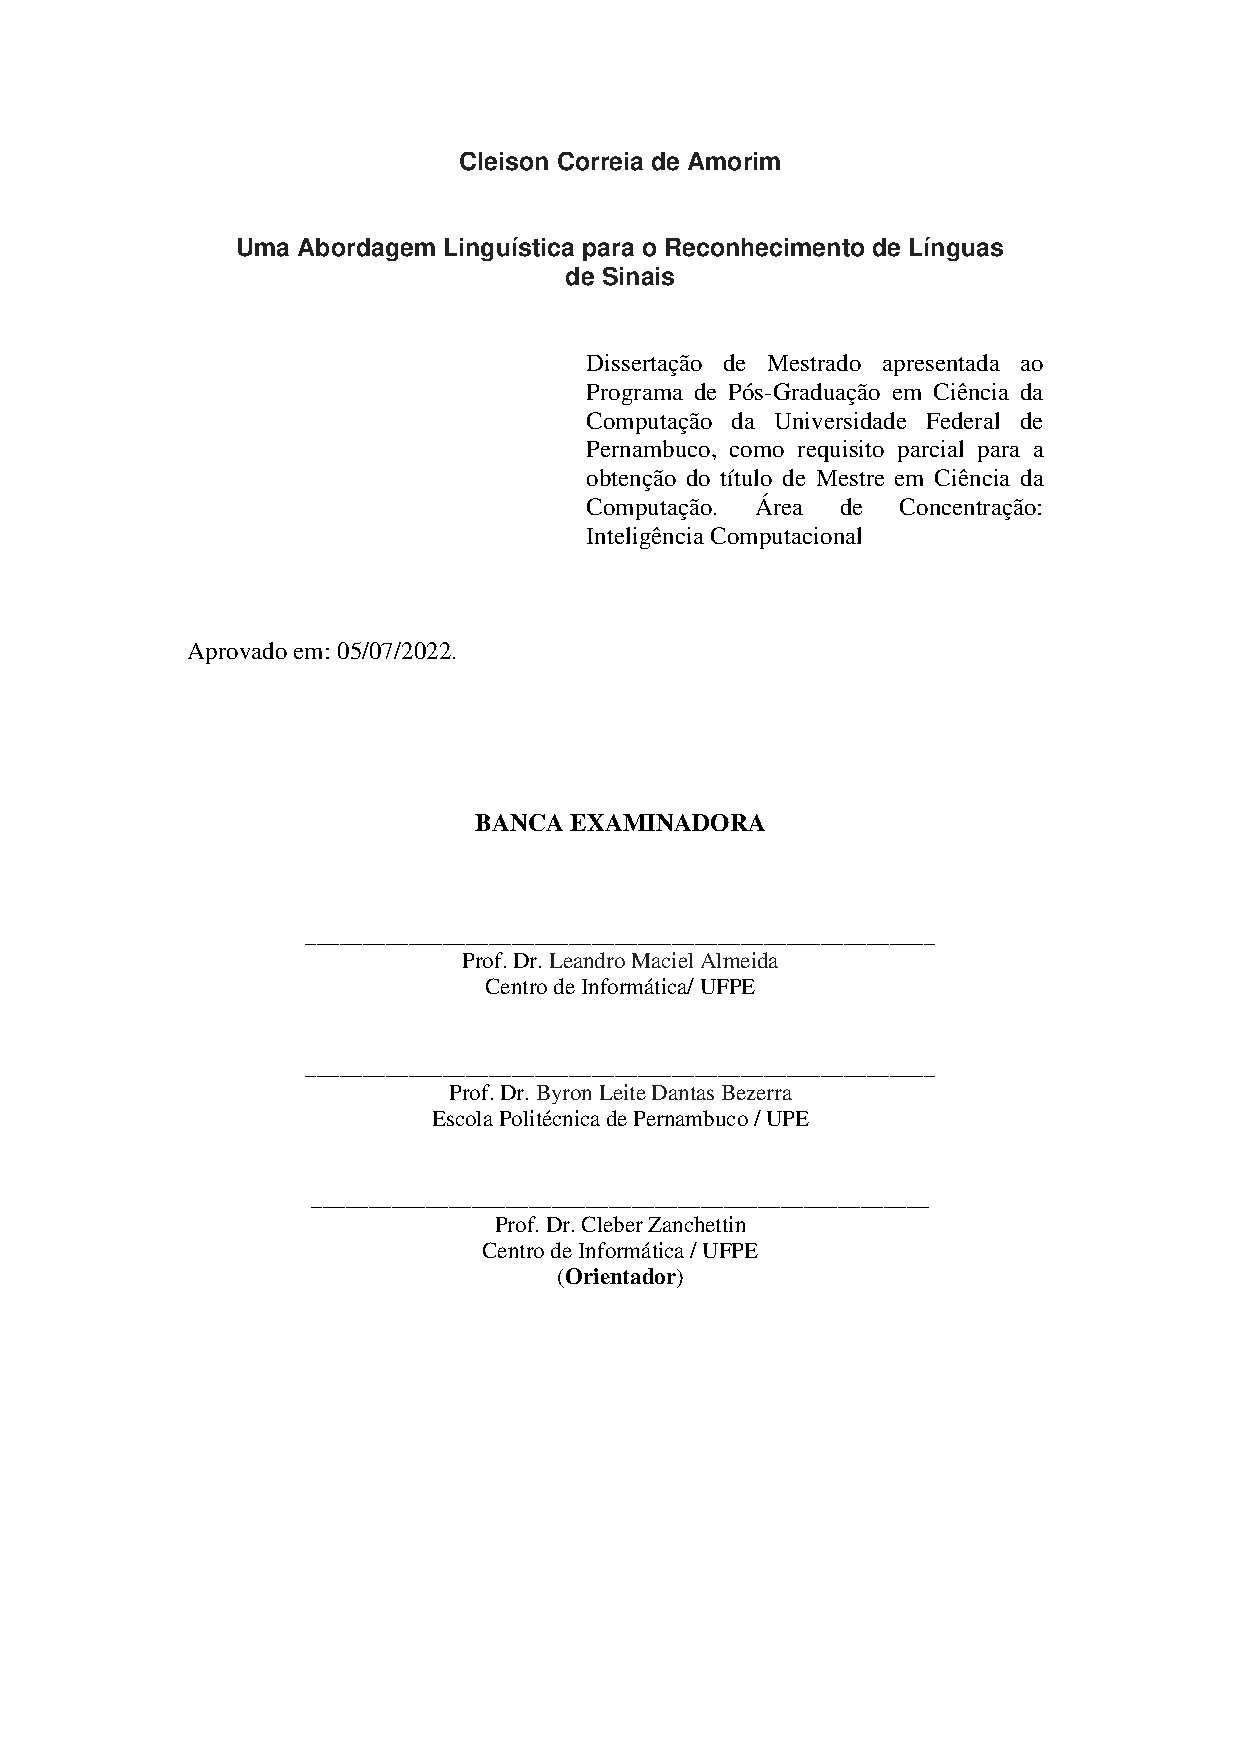
\includepdf[pages=-]{outros/biblioteca/folha_aprovacao}

% ----------------------------------------------------------
% DEDICATÓRIA
% ----------------------------------------------------------
\begin{dedicatoria}
   \vspace*{\fill}
   % \centering
   % \noindent
   \textit{
      Dedico este trabalho ao meu pai, que partiu ao longo da jornada deste mestrado, mas que deixou um grande exemplo de integridade e simplicidade pelo qual me espelharei em minha caminhada.
   }
\end{dedicatoria}
% ---

% ----------------------------------------------------------
% AGRADECIMENTOS
% ----------------------------------------------------------
\begin{agradecimentos}
Texto texto texto texto texto texto texto texto texto texto texto texto texto texto texto texto texto texto texto texto texto texto texto texto texto texto texto texto texto texto texto texto texto texto texto texto texto texto texto texto texto texto.

Texto texto texto texto texto texto texto texto texto texto texto texto texto texto texto texto texto texto texto texto texto texto texto texto texto texto texto texto texto texto texto texto texto texto texto texto texto texto texto texto texto texto.

Texto texto texto texto texto texto texto texto texto texto texto texto texto texto texto texto texto texto texto texto texto texto texto texto texto texto texto texto texto texto texto texto texto texto texto texto texto texto texto texto texto texto.

Texto texto texto texto texto texto texto texto texto texto texto texto texto texto texto texto texto texto texto texto texto texto texto texto texto texto texto texto texto texto texto texto texto texto texto texto texto texto texto texto texto texto.



\end{agradecimentos}
% ----------------------------------------------------------
% EPÍGRAFE

%Epígrafe: Elemento opcional e sem título em que o (a) autor (a) apresenta uma citação relacionada ao assunto tratado no trabalho. Deve ser elaborada conforme a ABNT-NBR 10520 (Citações). As citações de até três linhas devem estar entre aspas duplas e as citações com mais de três linhas devem ser destacadas com recuo de 4 cm da margem esquerda, com letra menor que a do texto e sem as aspas. A fonte da citação deve aparecer na lista de referências.
% ---------------------------------------------------------
\vspace*{\fill}

\begin{citacao}
  ``Conheça todas as teorias, domine todas as técnicas, mas ao tocar uma alma humana seja apenas outra alma humana.''
  (Carl Gustav Jung)
\end{citacao}

\newpage
% -----------------------------------------------------------
% PORTUGUÊS
% -----------------------------------------------------------
\begin{resumo}[Resumo]
  \noindent
  A língua de sinais é uma ferramenta essencial na vida do Surdo, capaz de assegurar seu acesso à comunicação, educação e desenvolvimento cognitivo e socio-emocional.
  Na verdade, ela é a principal força que une essa comunidade e o símbolo de identificação entre seus membros.
  Contudo, atualmente o número de indivíduos ouvintes que conseguem se comunicar por meio dessa língua é pequeno e, na prática, isso impõe obstáculos ao cotidiano do Surdo.
  Tarefas simples como utilizar o transporte público, comprar roupas, ir ao cinema ou obter assistência médica acabam tornando-se um desafio por conta dessa limitação.
  O Reconhecimento de Língua de Sinais é uma das áreas de pesquisa que objetiva desenvolver tecnologias capazes de reduzir essas barreiras linguísticas e facilitar a comunicação entre ambos indivíduos.
  Apesar disso, ao analisar sua evolução ao longo das últimas décadas, percebe-se que seu progresso ainda não é suficiente para disponibilizar soluções efetivamente aplicáveis ao mundo real.
  Isso ocorre principalmente porque várias pesquisas na área acabam não apropriando-se ou abordando adequadamente as particularidades linguísticas das línguas de sinais, decorrentes de sua natureza visual.
  Tendo isso em vista, este trabalho apresenta uma abordagem que aplica modelos sequenciais de aprendizagem de máquina para realizar o reconhecimento computacional dos sinais através de seus atributos linguísticos. Além disso, são introduzidos dois novos \textit{datasets} para a língua de sinais, dentre os quais está um \textit{dataset} de atributos linguísticos computados a partir do ASLLVD.
  Com isso, objetiva-se estabelecer uma direção capaz de conduzir a avanços mais efetivos para essa área e, consequentemente, contribuir com a superação dos obstáculos hoje enfrentados pelo Surdo.

  \vspace{\onelineskip}

  \noindent
  \textbf{Palavras-chaves}: Língua de Sinais. Linguística. Processamento de Linguagem Natural.
\end{resumo}



% -----------------------------------------------------------
% INGLÊS
% -----------------------------------------------------------
\begin{resumo}[Abstract]
  \begin{otherlanguage*}{english}
    \noindent
    Sign language is an essential resource to ensure the Deaf to have access to communication, education, as well as to cognitive and socio-emotional development. In fact, it is the main force that unites such community and the key trait that identifies its members.
    On the other hand, the number of hearing individuals who are able to communicate through this language is currently small and, in practice, this imposes obstacles to the daily life of the Deaf.
    Simple tasks like using public transportation, shopping for clothes, going to the movies, or getting medical assistance end up becoming challenges due to such limitation.
    The Sign Language Recognition, in turn, is one of the research areas dedicated to developing technologies that aim to reduce such language barriers and facilitate the communication between these individuals.
    However, when analyzing its evolution over the last decades, we realize that it has not progressed enough to provide solutions effectively applicable to the real world.
    This is mainly because several researches in this field do not appropriate or address the linguistic particularities presented by the sign languages, which stem from their visual nature.
    Considering this problem, the present work introduces an approach that adopts sequential machine learning models to recognize signs through their linguistic attributes. In addition, we introduce two new sign language datasets, among which is a novel dataset of linguistic attributes computed from the ASLLVD.
    Thus, we aim to establish a direction that can lead to more effective advances in this research area and, consequently, contribute to overcoming the obstacles faced by the Deaf today.

    \vspace{\onelineskip}

    \noindent
    \textbf{Keywords}: Sign Language. Linguistics. Natural Language Processing.
  \end{otherlanguage*}
\end{resumo}



% ----------------------------------------------------------
% LISTA DE FIGURAS
% ----------------------------------------------------------
\pdfbookmark[0]{\listfigurename}{lof}
\listoffigures*
\cleardoublepage


% ----------------------------------------------------------
% LISTA DE CÓDIGOS
% ----------------------------------------------------------
\lstdefinelanguage{ASLDataset}{
  sensitive=true,
  commentstyle=\color{greencomment},
  breaklines=true,
  keywords={ x, y, z },
  otherkeywords={ label, gloss, consultant, session, scene, frame_start, frame_end, passive_arm, fps, mode, name, value, score, frames, frame_index, handshape_dh, handshape_dh_start, handshape_dh_end, handshape_ndh, handshape_ndh_start, handshape_ndh_end, phono_attributes, skeleton, movement_dh, movement_ndh, orientation_dh, orientation_ndh, non_manual, mouth_opening, body, face, hand_left, hand_right },
  keywordstyle=\color{blue},
  upquote=true,
  stringstyle=\color{purple},
  showstringspaces=false,
  morestring=[b]',
  morestring=[b]",
  comment=[l]{//},
  morecomment=[s]{/*}{*/},
  literate=
    *{0}{{{\color{teal}0}}}{1}
    {1}{{{\color{teal}1}}}{1}
    {2}{{{\color{teal}2}}}{1}
    {3}{{{\color{teal}3}}}{1}
    {4}{{{\color{teal}4}}}{1}
    {5}{{{\color{teal}5}}}{1}
    {6}{{{\color{teal}6}}}{1}
    {7}{{{\color{teal}7}}}{1}
    {8}{{{\color{teal}8}}}{1}
    {9}{{{\color{teal}9}}}{1}
    {.}{{{\color{teal}.}}}{1}
}

\lstdefinestyle{mystyle}{
  backgroundcolor=\color{graybackground},
  basicstyle=\fontsize{9}{9}\ttfamily,
  captionpos=t,
  keepspaces=true,
  numbers=left,
  numbersep=10pt,
  numberstyle=\tiny\color{gray},
  showspaces=false,
  showstringspaces=false,
  showtabs=false,
  tabsize=4,
  frame=single,
  rulecolor=\color{gray},
}

\lstset{style=mystyle}


% Altera o nome padrão do rótulo usado no comando \autoref{}
\renewcommand{\lstlistingname}{Código-fonte}

% Altera o rótulo a ser usando no elemento pré-textual "Lista de código"
\renewcommand{\lstlistlistingname}{Lista de códigos-fontes}

\pdfbookmark[0]{\lstlistlistingname}{lol} % caso não tenha código fonte, comente esta linha 
\counterwithout{lstlisting}{chapter}

% Configura a 'Lista de Códigos' conforme as regras da ABNT (para abnTeX2)
\begingroup\makeatletter
\let\newcounter\@gobble\let\setcounter\@gobbletwo
\globaldefs\@ne \let\c@loldepth\@ne
\newlistof{listings}{lol}{\lstlistlistingname}
\newlistentry{lstlisting}{lol}{0}
\endgroup

\renewcommand{\cftlstlistingaftersnum}{\hfill--\hfil}

\let\oldlstlistoflistings\lstlistoflistings
{
  \let\oldnumberline\numberline
  \newcommand{\algnumberline}[1]{Código-fonte~#1~\enspace--~\enspace}
  \renewcommand{\numberline}{\algnumberline}

  \begin{KeepFromToc}
    \lstlistoflistings
  \end{KeepFromToc}
}
\cleardoublepage



% ----------------------------------------------------------
% LISTA DE QUADROS
% ----------------------------------------------------------
% \pdfbookmark[0]{\listofquadrosname}{loq} % caso não tenha quadros, comente esta linha 
% \listofquadros* % caso não tenha quadros, comente esta linha 
% \cleardoublepage



% ----------------------------------------------------------
% LISTA DE TABELAS
% ----------------------------------------------------------
\pdfbookmark[0]{\listtablename}{lot}
\listoftables*
\cleardoublepage




% ----------------------------------------------------------
% LISTA E ABREVIATURAS E SIGLAS
% ----------------------------------------------------------
%\printglossary[type=\acronymtype,title={\listadesiglasname},nonumberlist]
%\printglossaries
% compile uma vez com o comando \printglossaries e depois compile novamente com o comando \printglossaries comentado para as páginas glossário e siglas serem ocultadas.


% \setglossarystyle{modsuper}
\printnoidxglossary[style=modsuper,type=\acronymtype,title={\listadesiglasname},nonumberlist]
% \printglossary[style=super, type=\acronymtype]
\cleardoublepage



% ----------------------------------------------------------
% LISTA DE SIMBOLOS
% ----------------------------------------------------------
% % ---

% ---
% inserir lista de símbolos
% ---
\begin{simbolos}
  \item[$ \gamma $] Letra grega Gama
  %\item[$ \Lambda $] Lambda
  %\item[$ \zeta $] Letra grega minúscula zeta
  \item[$ \in $] Pertence
%  \item[$ \infty$] Infinito
%  \item[$ \ge$] Maior ou Igual
  \item[$ \delta$] Delta
  \item[$ \theta$] Teta
  \item[$ \sigma$] Sigma
  \item[$ \mu$] Mi
  
\end{simbolos}
% ---



% ----------------------------------------------------------
% SUMÁRIO
% ----------------------------------------------------------
\pdfbookmark[0]{\contentsname}{toc}
\tableofcontents*
% \begingroup\intoctrue
% \tableofcontents*
% \endgroup
\cleardoublepage

% \setcounter{page}{13}
\setcounter{tocdepth}{2}
\setcounter{table}{0}



% ----------------------------------------------------------
% ELEMENTOS TEXTUAIS
% ----------------------------------------------------------
\textual
% Introdução
\chapter{Introdução}
\label{cap:introducao}

\section{Motivação}
\label{motivacao}

% TODO: corrigir 'deficiente auditivo' ??? -- de acordo com PNS (pg 40), é apenas aquele que tem: (1) Muita dificuldade de ouvir ou não consegue de modo algum ouvir
% *** Sugestão ***: Ao modificar para "surdo" x "Surdo", apontar referência:
% "Seguindo convenção proposta por James Woodward (1982), neste livro será  usado o termo “surdo” para se referir à condição audiológica de não ouvir, e o termo “Surdo” para se referir a um grupo particular de pessoas surdas que partilham  uma língua e uma cultura" \cite{pereira-2011-conhecimento-alem-sinais}. 

Segundo a \acrfull{oms}, 19\% da população mundial apresenta algum grau de perda auditiva -- ou seja, em meio a uma população de 7,7 bilhões de habitantes, 1,5 bilhões de indivíduos sofrem com perda auditiva. Dentre esses, 450 milhões referem-se a perda de grau moderado ou severo e que necessitam de acesso a cuidados auditivos e outros serviços de reabilitação -- é o que nos revela o \textit{World Report on Hearing} (Relatório Mundial sobre Audição) publicado em 2021~\cite{who-2021-report-hearing}.

% Conforme o mundo alcança 10 bilhões de habitantes até 2050, a \acrshort{oms} estima que esse 2,5 bilhões de indivíduos (ou 25\% da população mundial) viverão com perda auditiva, dentre os quais 700 milhões serão perda de grau moderado ou severo~\cite{who-2021-report-hearing, opas-2021-oms-estima}.

% O mundo possui hoje 7,7 bilhões de habitantes, dentre os quais 1,5 bilhões de indivíduos possuem perda auditiva (o que equivale a 19\% da população mundial), sendo 450 milhões perda auditiva de moderada ou severa -- é o que aponta a \acrfull{oms} através do seu \textit{World Report on Hearing} (Relatório Mundial sobre Audição) publicado em 2021~\cite{who-2021-report-hearing}.

% Conforme a população mundial cresce para cerca de 10 bilhões de habitantes em 2050, estima-se que 2,5 bilhões de pessoas terão perda auditiva, dentre os quais 700 milhões serão de grau moderado ou elevado e necessitarão de acesso a cuidados auditivos e outros serviços de reabilitação~\cite{who-2021-report-hearing, opas-2021-oms-estima}

No Brasil, o panorama é de 10,7 milhões de habitantes com perda auditiva (ou 5\% da população), dos quais 2,3 milhões correspondem a perda moderada ou severa~\cite{ebc-2019-10-milhoes-pessoas, ibge-2021-pns, ibge-2021-projecao-populacao}. De acordo com o Instituto Locomotiva e o \citeauthor{ibge-2021-pns}, há uma homogeneidade entre homens e mulheres nessa população (54\% homens e 46\% mulheres), mas uma concentração maior nas regiões Sudeste (42\%) e Nordeste (26\%), seguidas pelo Sul (19\%), Norte (7\%) e Centro-Oeste (6\%). Além disso, como a perda auditiva é adquirida ao longo da vida em 91\% dos casos e agrava-se com o passar dos anos, nota-se uma predominância de indivíduos na faixa dos 60 anos de idade ou mais (57\%)~\cite{ebc-2019-10-milhoes-pessoas, ibge-2021-pns}.

Ainda de acordo com a \acrshort{oms}, as últimas décadas testemunharam avanços revolucionários no diagnóstico e reabilitação de problemas auditivos, como no campo da tecnologia auditiva, diagnóstico e telemedicina, com inovações que permitem que perdas e doenças relacionadas à audição sejam identificadas em qualquer idade e ambiente. Gestão médica e cirúrgica, aparelhos auditivos, implantes cocleares, terapia de reabilitação, linguagem de sinais e legendagem são exemplos de soluções que podem garantir que pessoas com doenças de ouvido ou com perda auditiva tenham acesso à educação e comunicação e, assim, tenham a oportunidade de cumprir seu potencial~\cite{who-2021-report-hearing}.

% Ao analisar dispositivos e intervenções capazes de auxiliar no diagnóstico e reabilitação dessas pessoas, a \acrshort{oms} afirma que as últimas décadas testemunharam avanços revolucionários, como no campo da tecnologia auditiva, diagnóstico e telemedicina, com inovações que permitem que perdas e doenças relacionadas à audição sejam identificadas em qualquer idade e ambiente. Gestão médica e cirúrgica, aparelhos auditivos, implantes cocleares, terapia de reabilitação, linguagem de sinais e legendagem são exemplos de soluções que podem garantir que pessoas com doenças de ouvido ou com perda auditiva tenham acesso à educação e comunicação e, assim, tenham a oportunidade de cumprir seu potencial~\cite{who-2021-report-hearing}.


No entanto, há uma disparidade no acesso a esses recursos, uma vez que a grande maioria das pessoas com perda auditiva não consegue acessá-los por viver em locais de baixa renda, onde profissionais especializados e serviços para cuidados auditivos não estão comumente disponíveis~\cite{who-2021-report-hearing}. Segundo a \citeauthor{opas-2021-oms-estima}, 78\% desses países têm menos de um otorrinolaringologista, 93\% têm menos de um audiologista, 83\% têm menos de um fonoaudiólogo, e 50\% têm menos de um professor para deficientes auditivos por milhão de habitantes. Mesmo em países com proporções relativamente altas desses profissionais, há uma distribuição desigual e isso não só representa desafios para as pessoas que precisam de atenção, mas também impõe demandas excessivas aos quadros que prestam esses serviços~\cite{opas-2021-oms-estima}.

%\begin{quote}
%    Entre os países de baixa renda, cerca de 78\% têm menos de um especialista em ouvido, nariz e garganta por milhão de habitantes; 93\% têm menos de um audiologista por milhão; apenas 17\% têm um ou mais fonoaudiólogos por milhão; e 50\% têm um ou mais professores para pessoas com deficiência auditiva por milhão. Mesmo em países com proporções relativamente altas de profissionais de saúde auditiva e de ouvido, há distribuição desigual de especialistas. Isso não só representa desafios para as pessoas que precisam de atenção, mas também impõe demandas excessivas aos quadros que prestam esses serviços~\cite{opas-2021-oms-estima}.
%\end{quote}

Marcos Sarvat, membro da Câmara Técnica de Cirurgia de Cabeça e Pescoço e Otorrinolaringologia do \acrfull{cfm}, ratifica que esse problema na assistência à saúde para deficientes auditivos é acentuado em países subdesenvolvidos, entre os quais está o Brasil. Segundo ele, é difícil o acesso à prevenção por meio de exames periódicos, bem como às consultas, aos medicamentos, às cirurgias e às próteses~\cite{ebc-2021-oms-estima}. Ele destaca ainda que essa falta de cuidados adequados gera deficiências estruturais, que resultam numa pior qualidade de vida que se estende a todas as gerações:

% Marcos Sarvat, membro da Câmara Técnica de Cirurgia de Cabeça e Pescoço e Otorrinolaringologia do \acrfull{cfm}, ratifica que o problema na assistência à saúde para as pessoas com perda de audição é acentuado nos países subdesenvolvidos, entre os quais está o Brasil. Segundo ele, é difícil o acesso à prevenção por meio de exames periódicos, bem como às consultas, aos medicamentos, às cirurgias e às próteses~\cite{ebc-2021-oms-estima}. Ele destaca ainda que essa falta de cuidados adequados à saúde auditiva gera deficiências estruturais, que resultam numa pior qualidade de vida que se estende a todas as gerações:

\begin{citacao}
    {[\dots]} isso reflete na educação das crianças. Uma criança que ouve mal aprende mal e se torna um adulto menos capaz do que seria, e assim por diante. Temos uma cascata de efeitos do idoso abandonado, do idoso solitário, da depressão, da perda de motivação, do desvínculo familiar, da perda de condições de trabalho. Tudo isso vem em cascata e é ignorado~\cite{ebc-2021-oms-estima}.
\end{citacao}

% TODO: revisar 'surdo' aqui:
Reflexos dessas deficiências estruturais são também encontrados na dificuldade de acesso a oportunidades básicas por esses indivíduos, como educação (dados de 2019 mostram que apenas 6\% concluíram o ensino superior; 14\% o ensino médio, 8\% o ensino fundamental e 71\% não possuem grau de instrução) e emprego (apenas 25\% estão no mercado de trabalho)~\cite{ibge-2021-pns}. Além disso, a grande maioria (87\%) não utiliza aparelhos auditivos porque são caros e inacessíveis. Renato Meirelles, que é presidente do Instituto Locomotiva, comenta:

\begin{citacao}
    {[\dots]} como a população surda teve menos oportunidade de estudar do que a população ouvinte; como tem mais dificuldade no mercado de trabalho do que a população ouvinte; o dinheiro para conseguir o aparelho é ainda mais difícil. Esse conjunto de preconceitos que existe na sociedade acaba criando um círculo vicioso que não possibilita que os surdos e os ouvintes tenham as mesmas oportunidades de se dar bem na vida~\cite{ebc-2019-10-milhoes-pessoas}.
\end{citacao}


Em meio a esses desafios que limitam o acesso aos cuidados e tecnologias adequados para reabilitação desses indivíduos, a língua de sinais acaba sobressaindo-se como uma alternativa que é mais inclusiva -- isso porque impõe menos barreiras ao não demandar investimento financeiro elevado ou a disponibilidade de profissionais especializados no serviço público de saúde pelo país. Apesar disso, ela é capaz de assegurar o desenvolvimento cognitivo, facilitar a comunicação, e possibilitar que crianças com deficiência auditiva obtenham educação e desenvolvimento socio-emocional adequado~\cite{who-2021-report-hearing}. % TODO: adicionar mais aqui
É possível aprender línguas de sinais por meio da própria família, da comunidade surda ou de recursos como livros, cursos, vídeos e materiais disponibilizados muitas vezes gratuitamente pela internet ou em escolas da rede pública de educação e institutos de surdos -- entre os quais o \acrfull{ines} é talvez o mais antigo, fundado em 1857~\cite{pereira-2011-conhecimento-alem-sinais}. 


% é capaz de assegurar o desenvolvimento cognitivo, facilitar a comunicação, e possibilitar que crianças obtenham educação e desenvolvimento socio-emocional adequado~\cite{who-2021-report-hearing}. Ela torna-se mais acessível porque não demanda investimento financeiro elevado ou que profissionais especializados estejam disponíveis de forma igualitária sobretudo no serviço público de saúde pelo país -- é possível aprender a língua de sinais através da própria família, da comunidade surda ou por meio de cursos, livros e outros recursos disponibilizados de forma gratuita na internet, em escolas públicas ou em institutos de surdos -- como o \acrfull{ines}, em funcionamento desde 1857~\cite{pereira-2011-conhecimento-alem-sinais}.

No Brasil, a língua sinalizada oficial é a \acrfull{libras}, a que foi reconhecida como meio legal de comunicação e expressão pela Lei n° 10.436, de 24 de abril de 2002~\cite{brasil-2002-lei10436}. Através dessa lei, a língua passou a receber maior atenção por educadores e pesquisadores, fazendo crescer significativamente o número de adeptos e defensores de sua utilização~\cite{pereira-2011-conhecimento-alem-sinais}.

% TODO: revisar se há contradição aqui:
% No entanto, apesar do papel fundamental que essa língua é capaz de exercer na comunicação do deficiente auditivo, dados do \acrshort{ibge} revelam que nem todos esses indivíduos a conhecem -- no Brasil, apenas 13\% dos que possuem perda auditiva moderada e 61\% daqueles com perda severa conhecem a \acrshort{libras}~\cite{ibge-2021-pns}. Apesar de não haver um análise concreta das razões que conduzem a isso, pode-se enumerar alguns motivos que contribuem para tal: uma vez que a perda auditiva é adquirida ao longo da vida em 91\% dos casos e, muitos desses indivíduos já são oralizados e usuários do português, eles preferem continuar utilizando a própria fala (auxiliados por dispositivos auditivos ou implantes cocleares) ou adotar a leitura labial; em outra parcela, há resistência de muitos pais de crianças que nascem surdas ou perdem a audição muito cedo, os quais rejeitam a língua de sinais e impõem a oralização de seus filhos; por fim, pode haver ainda um deficit ao incorporar e preparar os professores para o ensino da \acrshort{libras} como parte da currículo regular, fazendo com que muitas indivíduos concluam seus estudos como analfabetos funcionais~\cite{lobato-2021-surdez-nao-sinonimo-libras, ebc-2019-10-milhoes-pessoas, senado-2019-baixo-alcance-lingua-sinais}.


Se por um lado a língua de sinais é uma poderosa ferramenta que permite a comunicação e o desenvolvimento cognitivo do deficiente auditivo; por outro lado ainda há um obstáculo relevante que os distancia de uma plena inclusão em sociedade: a escassez de ouvintes que conhecem a língua de sinais e conseguem se comunicam por meio dela~\cite{bragg-2019-slr-interdisciplinary}. De acordo com a \citeauthor{senado-2019-baixo-alcance-lingua-sinais}, a língua de sinais está restrita à comunidade surda e isso transforma atividades corriqueiras num grande desafio, levando eles ao isolamento. No transporte público, por exemplo, esses indivíduos não conseguem pedir ajuda, requisitar informações sobre as rotas ou ter acesso aos anúncios nos alto-falantes sobre mudanças nelas; no cinema, eles não podem assistir filmes nacionais, pois apenas filmes estrangeiros dispõem de legendas; em lojas, é raro encontrar vendedores preparados para interagir em língua de sinais; no serviço de saúde, os surdos perdem sua vez se não estiverem atentos à enfermeira que fala o nome do próximo paciente, além de estarem suscetíveis a situações ainda mais trágicas: ONGs dedicadas aos surdos afirmam que não são raros os casos em que pacientes saem de consultas com uma prescrição errada de medicamento porque o médico não entendeu quais eram os sintomas; no mercado de trabalho, é comum empresas contratarem esses indivíduos para cumprir as cotas exigidas em lei, mas não se preocuparem em saber como eles são -- eles são muitas vezes vistos como incapazes e são designados a tarefas secundárias~\cite{senado-2019-baixo-alcance-lingua-sinais}.


% Apesar disso, os surdos ainda estão longe de uma plena inclusão na sociedade: o grande obstáculo é a escassez de ouvintes que se comuniquem na língua de sinais. De acordo com a \citeauthor{senado-2019-baixo-alcance-lingua-sinais}, a \acrshort{libras} está restrita à comunidade surda e isso transforma atividades corriqueiras num grande desafio, levando o surdo ao isolamento. No transporte público, por exemplo, esses indivíduos não conseguem pedir ajuda, requisitar informações sobre as rotas ou ter acesso aos anúncios nos alto-falantes sobre mudanças nelas; no cinema, eles não podem assistir filmes nacionais, pois apenas filmes estrangeiros dispõem de legendas; em lojas, não é difícil encontrar vendedores despreparados para interagir em língua de sinais ou que demonstrem preconceito com esses indivíduos; no serviço de saúde, os surdos perdem vez se não estiverem atentos à enfermeira que chama o nome do próximo paciente e estão suscetíveis a situações que podem ser ainda mais trágicas: ONGs dedicadas aos surdos afirmam que não são raros os casos em que pacientes com problemas sérios de saúde saem de consultas com uma prescrição errada de remédio, porque o médico não entendeu quais eram os sintomas; no mercado de trabalho, é comum empresas contratarem os surdos para cumprir as cotas exigidas em lei, mas não se preocuparem em saber como eles são -- elas encaram os surdos como incapazes e os atribuem tarefas secundárias~\cite{senado-2019-baixo-alcance-lingua-sinais}.

Um passo importante para contribuir com a quebra dessas barreiras consiste na pesquisa e desenvolvimento de tecnologias de processamento de língua de sinais -- que inclui o reconhecimento, geração e tradução dessa língua. 
Por meio delas, é possível conectar usuários e não-usuários da língua sinalizada, provendo assistência à sua comunicação e permitindo que a mensagem seja compreendida pelos interlocutores independentemente da barreira linguística -- semelhante ao que se observa para diálogos envolvendo línguas não-visuais de nacionalidades distintas.
Segundo \citeauthor{bragg-2019-slr-interdisciplinary}, essas tecnologias também tornariam acessíveis aos usuários dessa língua recursos úteis ao nosso cotidiano e que ainda não estão disponíveis para eles, como os assistentes pessoais, que são limitados ao uso de comandos de voz e que poderiam passar a responder pessoas articulando sinais. Além disso, a tradução dos sinais para texto poderia permitir o uso de mecanismos de busca ou outros sistemas baseados em texto de uma forma mais amigável; o processo inverso, por sua vez, poderia substituir automaticamente conteúdo textual por animações em língua de sinais. Outras possibilidades incluiriam a transcrição automática de vídeos produzidos em língua de sinais -- o que permitiria, por exemplo, uma indexação e busca desse conteúdo; a interpretação em tempo real quando não há intérpretes humanos disponíveis; ou outras ferramentas e aplicativos educacionais~\cite{bragg-2019-slr-interdisciplinary}.


% These technologies would make voice-activated services newly accessible to deaf sign language users – for example, enabling the use of personal assistants (e.g., Siri and Alexa) by training them to respond to people signing. They would also enable the use of text-based systems – for example by translating signed content into written queries for a search engine, or automatically replacing displayed text with sign language videos. Other possibilities include automatic transcription of signed content, which would enable indexing and search of sign language videos, real-time interpreting when human interpreters are not available, and many educational tools and applications.

% reconhecimento, tradução e transcrição dessa língua para outros idiomas (e de outros idiomas para ela). Em sua essência, essas tecnologias visam prover assistência nessa comunicação permitindo que esses indivíduos compreendam-se mutuamente mesmo utilizando línguas distintas. É uma tarefa desafiadora que tem sido abordada de forma multidisciplinar no decorrer das últimas décadas por diferentes subáreas da Ciência da Computação. \cite{bragg-2019-slr-interdisciplinary}

% Um passo importante para contribuir com a quebra dessas barreiras consiste na pesquisa e desenvolvimento de tecnologias para o reconhecimento, tradução e transcrição dessa língua para outros idiomas (e de outros idiomas para ela). Em sua essência, essas tecnologias visam prover assistência nessa comunicação permitindo que esses indivíduos compreendam-se mutuamente mesmo utilizando línguas distintas. É uma tarefa desafiadora que tem sido abordada de forma multidisciplinar no decorrer das últimas décadas por diferentes subáreas da Ciência da Computação. \cite{bragg-2019-slr-interdisciplinary}



% Um passo importante para redução dessas barreiras na comunicação entre usuários e não-usuários da língua sinalizada compreende a pesquisa e desenvolvimento de tecnologias capazes de realizar o reconhecimento, tradução e transcrição dessa língua para outros idiomas e vice-versa. Essa é uma tarefa desafiadora que vem sendo abordada de forma multidisciplinar no decorrer das últimas décadas por subáreas da Ciência da Computação -- a exemplo do \acrfull{slr}, que aplica reconhecimento de padrões, visão computacional, processamento de linguagem natural e linguística para construir métodos e algoritmos objetivam identificar sinais produzidos e compreender seu significado~\cite{wadhawan-2021-slr-systems-review}.

% TODO: revisar se SLR deveria ser especificado aqui (ou falar de forma mais abrangente das pesquisas)
O \acrfull{slr} é uma das áreas de pesquisa empenhadas em contribuir para que tecnologias como essas sejam desenvolvidas. Trata-se de uma área colaborativa que envolve reconhecimento de padrões, visão computacional, processamento de linguagem natural e linguística para construir métodos e algoritmos capazes de identificar sinais produzidos e compreender seu significado~\cite{wadhawan-2021-slr-systems-review}. 
Apesar disso, \citeauthor{cooper-2011-slr} acreditam que o progresso apresentado por ela nas últimas décadas ainda foi pouco expressivo:

\begin{citacao}
    Enquanto sistemas de reconhecimento automático da fala avançaram ao ponto de estarem comercialmente disponíveis, o reconhecimento de sinais ainda está em sua infância. Atualmente, todos os serviços comerciais de tradução de sinais são baseados em humanos e requerem pessoal especializado -- o que os tornam caros~\cite[tradução nossa]{cooper-2011-slr}.
\end{citacao}

% \citeauthor{bragg-2019-slr-interdisciplinary} argumentam que 
%Current research in sign language processing occurs in disciplinary silos, and as a result does not address the problem comprehensively. For example, there are many computer science publications presenting algorithms for recognizing (and less frequently translating) signed content. The teams creating these algorithms often lack Deaf members with lived experience of the problems the technology could or should solve, and lack knowledge of the linguistic complexities of the language for which their algorithms must account. The algorithms are also often trained on datasets that do not reflect real-world use cases. As a result, such single-disciplinary approaches to sign language processing have limited real-world value [39].
%To overcome these problems, we argue for an interdisciplinary approach to sign language processing. Deaf studies must be included in order to understand the community that the technology is built to serve. Linguistics is essential for identifying the structures of sign languages that algorithms must handle. Natural Language Processing (NLP) and machine translation (MT) provide powerful methods for modeling, analyzing, and translating. Computer vision is required for detecting signed content, and computer graphics are required for generating signed content. Finally, Human-Computer Interaction (HCI) and design are essential for creating end-to-end systems that meet the community's needs and integrate into people's lives.

% Os autores acreditam que parte disso deve-se ao fato de que muitas pesquisas em \acrshort{slr} abordam o problema de forma incorreta: eles encaram o reconhecimento da língua de sinais como uma tarefa de reconhecimento de gestos, concentrando-se na identificação de características e métodos para rotular um sinal dentre um conjunto de possibilidades bem definidas -- porém, essas línguas vão muito além disso.


\citeauthor{bragg-2019-slr-interdisciplinary} e \citeauthor{cooper-2011-slr} acreditam que, de uma forma geral, isso está relacionado a fatores como os desafios particulares a essas línguas e a forma com que as pesquisas desenvolvidas na área têm abordando o problema no decorrer das últimas décadas.
Pode-se sumarizar esses fatores nos seguintes itens principais:

\begin{enumerate}
    % TODO: revisar esse contraponto ao reconhecimento da lingua de sinais
    \item Abordagem inadequada do problema: pesquisas atuais em processamento de língua de sinais ocorrem em silos disciplinares e, como resultado, não abordam o problema de uma forma holística. Por exemplo, muitas delas abordam o reconhecimento, mas poucas contemplam a tradução dos sinais em contextos reais ou consideram elementos como a linguística nesse processo.
    Há ainda pesquisas que abordam o problema como uma tarefa de reconhecimento de gestos e buscam identificar métodos para rotular um sinal dentre um conjunto de possibilidades bem definidas -- no entanto, essas línguas vão mais além do que uma coleção de gestos bem definidos.

    \item Natureza multicanal: línguas de sinais transmitem significado através de múltiplos canais ao mesmo tempo -- como por exemplo, a interação entre as mãos, a interação delas para com o corpo do interlocutor, suas orientações e configurações enquanto se movem, as expressões da face, olhos, cabeça e ombros, a intensidade com eles são articulados, entre outros que são abordados na linguística e que ocorrem simultaneamente.
    Isso significa que observar um canal isolado -- como observa-se em muitas pesquisas que contemplam apenas mãos estáticas ou fora do contexto -- é insuficiente para abordar corretamente a língua.
    
    \item Linguística particular: a linguística das línguas sinalizadas nos evidencia que elas possuem diversas particularidades atreladas à sua natureza visual, e isso torna muitas das técnicas hoje utilizadas no processamento das línguas faladas inadequadas a esse contexto.
    Sendo assim, ao invés de reproduzir técnicas empregadas às línguas faladas, é necessário que pesquisas em processamento de línguas sinalizadas desenvolvam técnicas próprias que explorem tais particularidades linguísticas e, com isso, que sejam capazes de contribuir avanços relevantes à área.
    %\item Linguística particular: já é evidente através dos estudos da linguística das línguas sinalizadas que suas particularidades enquanto línguas visuais tornam muitas das técnicas utilizadas para reconhecimento da fala inadequadas para o \acrshort{slr}. Dessa forma, não é correto simplesmente reproduzir abordagens de processamento de fala; mas é preciso compreender e desenvolver técnicas que levem em consideração tais particularidades.
    
    \item \textit{Datasets} limitados: os \textit{datasets} de língua de sinais disponíveis publicamente são limitados em quantidade e qualidade, e isso impõe um desafio relevante para as pesquisas na área. Técnicas modernas de aprendizagem de máquina demandam uma quantidade crescente de dados que representem o contexto de aplicação no mundo real. A escassez desses dados faz que os algoritmos desenvolvidos não sejam capazes de aprender corretamente sobre o domínio do problema e, consequentemente, não sejam capazes de generalizar soluções úteis para o mundo real.
    
\end{enumerate}


Tendo em vista essas lacunas, bem como os papel importante que as línguas de sinais podem desempenhar para auxiliar o deficiente auditivo a superar muitas das barreiras discutidas até aqui, este trabalho contribui introduzindo uma nova abordagem de processamento de sinais que considera a linguística dessas línguas e, consequentemente, sua natureza multicanal para realizar o processamento dos sinais. Além disso, aqui também são apresentados dois novos \textit{datasets} que podem suportar novas pesquisas a continuar evoluindo nessa direção.

%desafios encarados pelos deficientes visuais que foram apresentados até aqui, bem como encarados e o importante papel que as línguas de sinais podem desempenhar para auxiliar os deficientes auditivos a superar muitas dessas barreiras, esse trabalho introduz uma abordagem baseada na linguística para o processamento de línguas de sinais, bem como dois novos \textit{datasets} que visam contribuir com diversas outras pesquisas na área.




% Many approaches to SLR incorrectly treat the problem as Gesture Recognition (GR). So research has thus far focused on identifying optimal features and classification methods to correctly label a given sign from a set of possible signs. However, sign language is far more than just a collection of well specified gestures.
% Sign languages pose the challenge that they are multi-channel; conveying meaning through many modes at once. While the studies of sign language linguistics are still in their early stages, it is already apparent that this makes many of the techniques used by speech recognition unsuitable for SLR. In addition, publicly available data sets are limited both in quantity and quality, rendering many traditional computer vision learning algorithms inadequate for the task of building classifiers.
% However, even given the lack of translation tools, most public services are not translated into sign. There is no commonly-used, written form of sign language, so all written communication is in the local spoken language



% The use of computational approaches to help the learning, communication, translation, and interaction using sign language is essential to include this population in society. In the machine learning research area, Sign Language Recognition (SLR) refers to a collaborative field that involves pattern matching, computer vision, natural language processing, and linguistics [2] to enable sign language users to communicate with spoken languages users. However, while speech recognition systems have advanced to the point of being commercially available, SLR systems are still in very early stages. Therefore, commercial translation services for sign languages are human-based, require specialized personnel, and are often expensive [3].
% Among the main challenges involved, there is the scarcity of approaches structured around the linguistics of the sign language, the limitation in quantity and quality of public datasets that could lead to significant advancements of the SLR techniques, and the multi-channel nature of the language – which convey meaning through many modes at once [3].





% \cite{cooper-2011-slr}:
% While automatic speech recognition has now advanced to the point of being commercially available, automatic SLR is still in its infancy. Currently all commercial translation services are human based, and therefore expensive, due to the experienced personnel required.
% SLR aims to develop algorithms and methods to correctly identify a sequence of produced signs and to understand their meaning. Many approaches to SLR incorrectly treat the problem as Gesture Recognition (GR). So research has thus far focused on identifying optimal features and classification methods to correctly label a given sign from a set of possible signs. However, sign language is far more than just a collection of well specified gestures.
% Sign languages pose the challenge that they are multi-channel; conveying meaning through many modes at once. While the studies of sign language linguistics are still in their early stages, it is already apparent that this makes many of the techniques used by speech recognition unsuitable for SLR. In addition, publicly available data sets are limited both in quantity and quality, rendering many traditional computer vision learning algorithms inadequate for the task of building classifiers.
% However, even given the lack of translation tools, most public services are not translated into sign. There is no commonly-used, written form of sign language, so all written communication is in the local spoken language.


% \cite{wadhawan-2021-slr-systems-review}:
% Sign language recognition is a collaborative research area which involves pattern matching, computer vision, natural language processing, and linguistics. Its objective is to build various methods and algorithms in order to identify already produced signs and to perceive their meaning. Sign language recognition systems are Human Computer Interaction (HCI) based systems that are designed to enable effective and engaging interaction. These system follows a multidisciplinary approach of data acquisition, SL technology, SL testing and SL linguistics. Such a system can be deployed in public services like hotels, railways, resorts, banks, offices etc. to enable hearing impaired people learn new concepts and facts and to control emotional behavior [1].







% =======
% Baixo alcance da língua de sinais leva surdos ao isolamento
% https://www12.senado.leg.br/noticias/especiais/especial-cidadania/baixo-alcance-da-lingua-de-sinais-leva-surdos-ao-isolamento
% Fonte: Agência Senado
% -------
% Em 2002, a Lei 10.436 deu à Libras o status de meio legal de comunicação e expressão. Desde então, escolas, faculdades, repartições do governo e empresas concessionárias de serviços públicos estão obrigadas a providenciar intérpretes para atender aos surdos. A lei faz aniversário em 24 de abril, que, por isso, transformou-se no Dia Nacional da Língua Brasileira de Sinais.
% ------
% Apesar da lei de 2002, os surdos ainda estão longe da plena inclusão na sociedade. Como o curta Libras É Merda? denuncia (às avessas), o grande obstáculo é a escassez de ouvintes que se comuniquem na língua de sinais. A Libras está restrita à comunidade surda. Isso pode transformar atividades corriqueiras num inferno. No ônibus, os surdos não conseguem saber do cobrador qual é a parada em que devem descer. Se o alto-falante do aeroporto anuncia troca de portão, eles correm o risco de perder o avião caso não estejam com os olhos grudados nos telões de voos.
% No cinema, não podem ver filmes nacionais, pois só os estrangeiros são legendados. Na loja, o vendedor menos paciente e esclarecido pode confundir os gestos da língua de sinais com brincadeira ou deficiência mental e simplesmente virar as costas para os clientes surdos.
% Nos serviços de saúde, os surdos perdem a vez quando não estão atentos à enfermeira que grita o nome do próximo paciente. Essa dificuldade, aliás, levou à criação de um projeto-piloto no Sistema Único de Saúde (SUS): o Hospital Federal de Ipanema, no Rio de Janeiro, abriu uma central de atendimento e consulta mediada por intérprete de Libras.
% -----
% As situações podem inclusive ser trágicas. ONGs dedicadas aos surdos dizem que não são raros os casos em que pacientes com problemas sérios de saúde saem de consultas com uma prescrição errada de remédio, porque o médico não entendeu quais eram os sintomas, e situações em que inocentes são mortos porque não ouviram a ordem de parar e o policial atirou por não perceber que eram surdos.
% "Deficiente não é o surdo, mas a sociedade que não sabe se comunicar com ele. Se o surdo encontrasse no dia a dia pessoas que soubessem a língua de sinais, ele não enfrentaria tantas barreiras e, por isso, nem perceberia a surdez como deficiência" afirma a coordenadora do Laboratório de Educação de Surdos e Libras, da Universidade de Brasília (UnB), Edeilce Buzar.
% Segundo o Censo mais recente, viviam em 2010 no Brasil 2,1 milhões de pessoas que escutavam muito pouco ou nada — o equivalente à população de Manaus. A pesquisa do IBGE não apontou quantas faziam uso da língua de sinais.

% CENSO - IBGE 2018:
% - 5% (9,6 milhões) da população brasileira têm deficiência auditiva
% - 2,1 milhões são surdos ou escutam muito pouco
% - 7,5 milhões apresentam alguma dificuldade para ouvir
% - 360 milhões de pessoas sofrem algum tipo de surdez no mundo
% - 32 milhões são crianças
% - 31 milhões vivem em países em desenvolvimento

% As primeiras barreiras linguísticas por vezes são impostas pela própria família. Quando a criança nasce surda ou perde a audição ainda pequena, muitos pais rejeitam a língua de sinais e impõem a oralização. Sem ouvir a própria voz, o treinamento da fala e da leitura labial costuma ser lento e penoso. O aprendizado da língua de sinais, ao contrário, é natural para quem, compensando a lacuna da audição, tem na visão o sentido mais apurado.
% -----
% Raras escolas estão adaptadas para receber alunos surdos. A mera presença de um intérprete da língua de sinais ao lado do professor não é suficiente. Por um lado, muitas crianças surdas chegam ao colégio sem saber língua nenhuma e vão ter que aprender a Libras do zero. Por outro, as que já sabem a língua de sinais não encontram professores preparados para ensinar-lhes o português escrito. Nessa situação, como a Libras é a primeira língua do estudante, o português precisa ser apresentado como segundo idioma, com uma metodologia completamente diferente, tal como uma língua estrangeira. O professor precisa ser bilíngue e ter uma formação específica.
% Em consequência do despreparo das escolas, muitos surdos chegam ao fim dos estudos como analfabetos funcionais. É por isso, aliás, que tentar se comunicar por escrito com um surdo nem sempre dá certo.

% — Os surdos acabam sendo forçados a viver encapsulados em seus próprios mundos. São como almas que passam por nós sem que nos preocupemos em enxergá-los ou interagir com eles — compara o intérprete de Libras e ex-presidente da Associação de Pais e Amigos dos Deficientes Auditivos do Distrito Federal (Apada-DF) Marcos de Brito.
% -----
% Desde 1991, a Lei 8.213 obriga as empresas a reservar uma parte de suas vagas para funcionários com algum tipo de deficiência. Para firmas que tenham entre 100 e 200 trabalhadores, por exemplo, a cota é de 2%. A inclusão efetiva nem sempre ocorre. Tarcísio Barroso, de 31 anos, ficou surdo ainda bebê, também por causa da meningite. Ele é oralizado, mas tem a Libras como primeira língua. Mesmo pós-graduado na área da tecnologia da informação, acabou sendo relegado a tarefas secundárias em muitas das empresas onde trabalhou, em Brasília.
% — A comunicação com meus chefes sempre foi falha. Alguns não se preocupavam em articular bem as palavras na hora de falar, para eu fazer a leitura labial. Outros preferiam se comunicar por escrito, mas usavam palavras difíceis ou frases pouco objetivas, o que dificultava a minha compreensão. De tanto eu pedir que explicassem novamente cada orientação, acabavam concluindo que eu tinha deficiência intelectual e passavam a me deixar de lado. Já chorei muito por causa disso.
% A mãe dele, Vanilda Barroso, lembra que a inadequação que ele agora sente no trabalho é muito parecida com a que sentia no colégio, quando os professores não exploravam as suas potencialidades e só apontavam as dificuldades.
% — As empresas contratam um surdo e nem se preocupam em saber como os surdos são. Só querem cumprir a cota exigida pela lei. Não estão interessadas na inclusão — ela afirma. — E a inclusão não é difícil. Bastaria que as empresas deixassem de encarar o surdo como um incapaz e passassem a vê-lo como um estrangeiro que não compreende plenamente o português e precisa de explicações numa linguagem mais clara.



% ==============
% IBGE confirma: surdez não é sinônimo de Libras
% https://desculpenaoouvi.com.br/ibge-confirma-surdez-nao-e-sinonimo-de-libras/?fbclid=IwAR1Z5mcQeTlaaVCuEtDXDQoLW9cwT17yBplyQUgFF7NXxM7qT5saMTjFaWk
% 
% IBGE - Pesquisa Nacional de Saúde (PNS) - 2019:
% - 8,4% (17,3 milhões) da população com 2+ anos com algum grau de deficiência
%
% Com deficiência auditiva:
% - 1,3% da população em idade de trabalhar (14+ anos)
% - 2,6% da população fora da força de trabalho
%
% Nível de ocupação: 
% - 25,4% das pessoas de 14+ anos
% 
% Nível de instrução (pessoas com 18+ anos): 
% - 67,6% sem instrução e fundamental incompleto
% - 10,8% fundamental completo e médio incompleto
% - 16,6% médio completo e superior incompleto
% - 5% superior completo
%
% Uso de tecnologias auditivas:
% - 0,8% da população 2+ anos
% - 3,1% da população 60+ anos
%
% Uso da Libras (população 5+ anos) por grau de dificuldade para ouvir
% - Alguma dificuldade: 1,8% sabe usar
% - Muita dificuldade: 3,0% sabe usar
% - Não consegue de modo algum: 35,8% sabe usar
% --> "com deficiência auditiva" (grande dificuldade + não consegue de modo algum): 22,4%

% “Além disso, a informação [PNS] é importante para não generalizar as pessoas com deficiência auditiva: ao analisar os dados, é possível perceber que nem todos sabem se comunicar em Libras, pois fazem uso da fala, se comunicam oralmente, muitos deles com o apoio da leitura labial. Portanto, precisam de outros recursos de acessibilidade, como por exemplo as legendas, além de necessitarem de propostas educacionais distintas”, diz a pesquisadora.
% Comprovadamente, acessibilidade para surdos não se resume à interpretação em Libras e, como mostrado pelo IBGE, não atende a necessidade da maioria.

% -----
% Esses dados são essenciais para que se desmistifique que surdez é sinônimo de ser usuário exclusivo da Libras. A Libras tem função fundamental na comunicação de uma parcela de pessoas Surdas, assim como a Língua Portuguesa também tem função fundamental para a grande maioria das pessoas com deficiência auditiva.
% -----
% Não podemos continuar com políticas como as que vêm sendo implementadas nos últimos 10 anos, onde a iniciativa pública e privada decidem erroneamente que basta incluir Libras e todos os surdos serão contemplados com ela.
% -----
% Graças à Pesquisa Nacional de Saúde de 2019 realizada pelo IBGE, podemos afirmar categoricamente que A SURDEZ É PLURAL e as formas de acessibilidade também devem ser.



% =====
% Painel de Indicadores de Saúde – Pesquisa Nacional de Saúde
% https://www.pns.icict.fiocruz.br/painel-de-indicadores-mobile-desktop/


% =====
% País tem 10,7 milhões de pessoas com deficiência auditiva, diz estudo
% https://agenciabrasil.ebc.com.br/geral/noticia/2019-10/brasil-tem-107-milhoes-de-deficientes-auditivos-diz-estudo
% ------

% Instituto Locomotiva + Semana da Acessibilidade Surda:
% - 10,7 milhões de pessoas com deficiência auditiva (Brasil)
%    - Dessas, 2,3 milhões têm deficiência severa
%       - 15% já nasceram surdos
%
% - A surdez atinge 54% de homens e 46% de mulheres
% - A predominância (57%) é na faixa de 60+ anos
% 
% Condição nascida x adquirida:
% - 9% das pessoas nasceram 
% - 91% adquiriram ao longo da vida (metade foi antes dos 50 anos)
% 
% Do total pesquisado:
% - 87% não usam aparelhos auditivos (13% utilizam)

% ------
% “A deficiência auditiva é uma deficiência que se agrava com o passar dos anos. E como o Brasil está passando por um processo de envelhecimento da população, hoje já temos 59 milhões de brasileiros com mais de 50 anos e, em 2050, vamos chegar com mais de 98 milhões de brasileiros com mais de 50 anos de idade, essa é uma tendência que só vai crescer”, disse Renato Meirelles, presidente do Instituto Locomotiva. Completou que a “sociedade, claramente, não está preparada para isso”.

% ------
% Dois em cada três brasileiros 
% - 66,6% relataram enfrentar dificuldades nas atividades do cotidiano
% --> “Com isso, eles se divertem menos, têm menos chance no mercado de trabalho, não têm as mesmas oportunidades educacionais que os ouvintes têm”. 
% -----
% A falta de acolhimento e inclusão limitam o acesso dos surdos às oportunidades básicas, como educação
% - somente 7% têm ensino superior completo
% - 15% frequentaram até o ensino médio
% - 46% até o fundamental
% - 32% não possuem grau de instrução
% -------
% - 20% das pessoas com deficiência auditiva idosos não conseguem sair sozinhas
% - 37% estão no mercado de trabalho
% - 87% não usam aparelhos auditivos
% --> “Porque é muito caro e inacessível para a maioria dessa população”, disse Meirelles. “E como a população surda teve menos oportunidade de estudar do que a população ouvinte, como tem mais dificuldade no mercado de trabalho do que a população ouvinte, o dinheiro para conseguir o aparelho é ainda mais difícil. Esse conjunto de preconceitos que existe na sociedade acaba criando um círculo vicioso que não possibilita que os surdos e os ouvintes tenham as mesmas oportunidades de se dar bem na vida.”
% --> “Quando comecei no meu trabalho, as pessoas pensavam que eu não era capaz de fazer as coisas. Demorou demais para que elas acreditassem que eu tinha capacidades, mas às vezes ainda me olham com discriminação e desconfiança por eu ser quem sou”, afirmou uma mulher com deficiência auditiva de 30 anos, entrevistada em São Paulo.

% ------
% Entre os tipos de ocupação desempenhada pelas pessoas com deficiência auditiva com 18+ anos:
% - 43% empregado no setor privado 
% - 37% trabalhador por conta própria
%
% Segundo Renato Meirelles, “essas pessoas desistiram de arrumar emprego e passaram a empreender para garantir o seu sustento”.
% A pesquisa foi realizada entre os dias 1º e 5 de setembro passado, com 1,5 mil brasileiros surdos e ouvintes. No total, o Brasil possui 50,3 milhões de pessoas com deficiência. 

% -----
% A pesquisa mostra que a maior parcela de pessoas com deficiência auditiva está:
% - 42%: Região Sudeste
% - 26%: Nordeste 
% - 19%: Sul
% - 6%: Centro-Oeste 
% - 7%: Norte

% Das pessoas com deficiência auditiva:
% - 28% declararam ter também algum tipo de deficiência visual
% - 2% deficiência intelectual.

% Dos brasileiros com problemas auditivos:
% 14% não se sentem à vontade e poder falar sobre quase tudo com a família (11% da população de forma geral)
% 40% sentem isso em relação a amigos (34% da população de forma geral)
% A sondagem revela, ainda, que pessoas com deficiência auditiva severa têm três vezes mais chance de sofrerem discriminação em serviços de saúde do que pessoas ouvintes.

% -----
% Segundo a Organização Mundial da Saúde (OMS) existem 500 milhões de surdos no mundo e, até 2050, haverá pelo menos 1 bilhão em todo o globo. 





% =====
% Livro lingua de sinais
% https://books.google.com.br/books?hl=pt-BR&lr=&id=JVVYWP6btj4C&oi=fnd&pg=PA9&dq=lingua+de+sinais&ots=paEl9LqTn7&sig=-xCW5BpO6r8eNs7R8OtSymDrdjU#v=onepage&q=lingua%20de%20sinais&f=false


% https://www.scielo.br/j/es/a/LScdWL65Vmp8xsdkJ9rNyNk/?format=pdf&lang=pt

\section{Objetivos}
\label{sec:introducao-objetivos}

O objetivo geral deste trabalho consiste em propor uma abordagem de \acrlong{slr} baseada na linguística, a qual considere as complexidades de sua natureza visual e preencha algumas das lacunas deixadas em aberto por pesquisas na área, afim de contribuir com avanços mais efetivos.

Como objetivos específicos, este trabalho busca alcançar:

\begin{itemize}
    \item Propor uma estratégia para computar atributos linguísticos a partir de \textit{datasets} existentes da língua de sinais;

    \item Disponibilizar um \textit{dataset} de atributos linguísticos, o qual atualmente é inexistente, para suportar o desenvolvimento de novas técnicas para as línguas de sinais;

    \item Identificar, aplicar e avaliar algoritmos que possibilitem abordar o reconhecimento da língua de sinais através de sua linguística, acomodando as complexidades de sua natureza visual.
    
\end{itemize}


\section{Metodologia}
\label{metodologia}

A metodologia aplicada nesta dissertação concentra-se em compreender os desafios atuais da área de pesquisa para assim introduzir uma proposta que suporte avanços futuros coerentes com as necessidades do mundo real.
As etapas percorridas aqui podem ser sumarizadas como:

\begin{itemize}
    \item Revisão do panorama atual da deficiência auditiva e do papel que as línguas de sinais desempenham aqui;
    \item Revisão do panorama das pesquisas atuais em processamento de língua de sinais e das lacunas que têm limitado progressos mais expressivos na área.
    \item Desenvolvimento de uma proposta que aborde as lacunas acima, contribuindo para preencher algumas delas e produzindo artefatos que suportem novas pesquisas a evoluir nessa direção;
    \item Realização de experimentos e análise dos resultados coletados.
\end{itemize}

% - análise do panorama atual das línguas de sinais 
% - análise do panorama atual das pesquisas na área e identificação de principais lacunas para seu avanço
% - revisão da literatura das línguas de sinais e de sua linguísticas
% - seleção de um conjunto de atributos linguísticos
% - análise de técnicas algébricas para suportar o processamento de atributos linguísticos selecionados
% - seleção de um modelos sequenciais de aprendizagem de máquina para os experimentos
% - execução dos experimentos e análise dos resultados coletados

\section{Organização do trabalho}
\label{organizacao-trabalho}



% Fundamentação
\chapter{Fundamentação teórica}
\label{cap:fundamentacao}

Este capítulo apresenta os principais conceitos necessários para compreender o contexto das línguas de sinais e a abordagem proposta por esta pesquisa.
Primeiro, introduziremos na \autoref{sec:lingua-sinais} uma discussão acerca do Surdo e da língua de sinais.
Em seguida, na \autoref{sec:linguistica}, nos aprofundaremos na linguística e nas particularidades dessa língua.
Na \autoref{sec:slr}, abordaremos o panorama atual e os desafios existentes para a área de \acrfull{slr}.
Por fim, na \autoref{sec:modelos-sequenciais}, discutiremos sobre os modelos sequenciais de \acrlong{dl}.


% Este capítulo apresenta os principais conceitos necessários para compreender o trabalho desenvolvido nesta pesquisa.
% Este capítulo aborda o conteúdo teórico necessário para desenvolver a solução para o problema descrito na introdução:

% Primeiro, abordaremos uma visão geral acerca dos Surdos e das línguas 
% Em seguida, ... 
% Por fim, ... 


% - Línguas de sinais
% - Linguística da língua de sinais
% - Estado atual do SLR (survey com avanços atuais)

% - Reconhecimento de línguas faladas e texto x línguas de sinais
% - NLP: discutir evolução no tempo das abordagens utilizadas (para texto e voz) 
% - Utilização da fonologia + semântica das palavras para reconhecimento?

% - Modelos sequenciais (aprendizagem de máquina)
%     - Transformer: breve introdução (arquitetura e funcionamento)
%     - RNNs (GRU, LSTM, etc)


\section{O Surdo e a língua de sinais}
\label{sec:lingua-sinais}

Segundo \citeonline{pereira-2011-conhecimento-alem-sinais}, a língua de sinais é a língua utilizada pela maioria dos Surdos em sua vida diária. Muito mais do que isso, ela é a principal força que une essa comunidade e o símbolo de identificação entre seus membros.


Quando utilizados os termos ``Surdo'' ou ``comunidade Surda'' (com ``s'' capitalizado) não nos referimos apenas a uma condição clínica, mas a um grupo de indivíduos que, além de possuírem perda auditiva, utilizam a língua de sinais como principal meio de comunicação e compartilham experiências culturais associadas à surdez e ao uso dessa língua. Esses elementos estão interconectados e não pode-se definir comunidade Surda sem considerá-los como um todo.

De fato, ter uma perda auditiva não significa que uma pessoa seja membro da comunidade Surda ou que automaticamente saiba sinalizar, embora certamente esses sejam requisitos importantes:


\begin{citacao}
    Não há como apontar uma pessoa sentada num saguão lendo uma revista e dizer: ``esta pessoa é Surda''. Ainda que ela esteja utilizando aparelhos auditivos, não há como saber com qual comunidade ela se identifica.

    De maneira semelhante, não importa se ela é europeia, afro-americana, asiática ou de outra etnia; sua idade não é relevante, tampouco sua classe social ou gênero; a comunidade Surda não é moldada por nenhuma dessas características.~\cite[tradução nossa]{stewart-2021-barrons-asl}

\end{citacao}


Há um aspecto cultural essencial acompanhado de um forte sentimento de identidade grupal, que fazem com que a surdez seja percebida como uma diferença e não como uma deficiência, reiteram \citeonline{pereira-2011-conhecimento-alem-sinais}.


Apesar disso, no decorrer da história os Surdos tiveram sua identidade estigmatizada e desvalorizada pela sociedade ouvinte, que não aceitava a língua de sinais. Segundo \citeonline{hill-2019-sign-languages}, há até relativamente pouco tempo dizia-se a esses indivíduos que sua forma de comunicação era inferior, quebrada, sem importância ou insuficiente. Os sistemas educacionais e a comunidade majoritariamente ouvinte fizeram prevalecer a utilização da língua falada, mesmo às custas da língua de sinais.

De fato, atitudes como essas ainda persistem. \citeonline{pereira-2011-conhecimento-alem-sinais} comentam que muitos ouvintes tentam  diminuir os Surdos para que eles vivam isolados, tendo de assumir a cultura ouvinte como se ela fosse a única existente. Ser ``normal'' significaria, portanto, poder ouvir e falar oralmente:


\begin{citacao}
    Os ouvintes não prestam atenção aos Surdos que se comunicam por meio da língua de sinais. Consequentemente, não acreditam que eles sejam capazes de estudar em faculdade ou realizar mestrado e  doutorado, por exemplo. \cite{pereira-2011-conhecimento-alem-sinais}
\end{citacao}

\begin{citacao}
    Os ouvintes veem os Surdos com curiosidade e, às vezes, zombam deles por serem diferentes. \cite{strobel-2016-cultura-surda}
\end{citacao}


São muitas as lutas pelas quais os Surdos têm atravessado mas que, sobretudo nos últimos anos, têm conduzido a vitórias importantes como o reconhecimento das línguas de sinais oficialmente como línguas em diversos países, o direito a tradutores e intérpretes em eventos e canais públicos de comunicação e o acesso a uma educação bilíngue para as crianças Surdas, entre outras conquistas. No Brasil, por exemplo, a \acrfull{libras} foi reconhecida como uma língua em 2002 e, nos Estados Unidos, a \acrfull{asl} foi reconhecida ainda em 1989 \cite{brasil-2002-lei10436,pereira-2011-conhecimento-alem-sinais, jay-2011-dont-just-sign}.



De acordo com \citeonline{hill-2019-sign-languages,pereira-2011-conhecimento-alem-sinais}, as línguas de sinais distinguem-se das línguas orais porque utilizam o canal visual-espacial em vez do oral-auditivo. Por esse motivo, são denominadas línguas de modalidade gestual-visual, onde a informação linguística é recebida pelos olhos e produzida no espaço pelas mãos, pelo movimento do corpo e pela expressão facial.
Devido a disso, acrescentam \citeonline{stewart-2021-barrons-asl}, não existe uma forma escrita conveniente para essas línguas, mas apenas glosas que representam uma aproximação do significado de seus sinais.

Elas são consideradas como línguas naturais, ou seja, aquelas que emergem naturalmente quando indivíduos se reúnem formando uma comunidade. Assim como ocorre para as línguas orais, não existe uma universalidade: cada país tem sua própria língua sinalizada e elas, por sua vez, refletem a cultura dos diferentes países em que são utilizadas.


Apesar das particularidades acima, línguas orais e línguas sinalizadas compartilham os mesmos princípios quanto ao fato de que possuem um léxico e uma gramática. Ou seja, ambas apresentam um conjunto de símbolos convencionais bem como um sistema de regras que rege a combinação desses símbolos em unidades maiores de significado.
Dessa forma, a seção seguinte explorará em maior profundidade esses elementos linguísticos presentes nas línguas de sinais.

\section{Linguística da língua de sinais}
\label{sec:linguistica}

\citeonline{quadros-2004-estudos-linguisticos} afirmam que a linguística é o estudo científico das línguas naturais e humanas. Trata-se de uma ciência que procura desvendar os princípios independentes da lógica e da informação que determinam essa linguagem, bem como todas as formas criativas da comunicação.
Ela busca respostas para problemas essenciais relacionados à linguagem como, por exemplo: ``qual a natureza da linguagem humana?'',  ``como a comunicação se constitui?'', ``quais os princípios que determinam a habilidade dos seres humanos de produzir e compreender a linguagem?''.


% ===================================================
% \cite{quadros-2004-estudos-linguisticos}
% ===================================================
% 
% A linguística é o estudo científico das línguas naturais e humanas.
% ---
% A linguística busca desvendar os princípios independentes da lógica e da informação que determinam a linguagem humana. Tais princípios são o que há de comum nos seres  humanos que possibilitam a realização das diferentes línguas. Portanto, nesse  sentido, a teoria linguística extrapola as questões do uso.  
% ---
% A linguística é uma ciência que busca respostas para problemas essenciais relacionados à linguagem  que precisam ser explicados: Qual a natureza da linguagem humana? Como  a comunicação se constitui? Quais os princípios que determinam a habilidade dos seres humanos em produzir e compreender a linguagem? A linguística desmembra tais questões com a finalidade de explicar os problemas e  elaborar uma teoria da linguagem humana e uma teoria da comunicação. 


Segundo \citeonline {stewart-2021-barrons-asl}, os primeiros estudos linguísticos sobre as línguas de sinais foram realizados pelo professor Dr. William C. Stokoe Jr. da Universidade de Gallaudet, em ~\citeyear{stokoe-1960-sl-structure}. 
Seu primeiro artigo, intitulado ``\textit{Sign Language Structure}'' (ou Estrutura da Língua de Sinais), foi seguido pela publicação do primeiro dicionário da \acrfull{asl} em \citeyear{stokoe-1965-dictionary-asl} -- o ``\textit{Dictionary of American Sign Language on Linguistic Principles}'' (ou Dicionário da Língua de Sinais Americana em Princípios Linguísticos) -- que foi compilado em parceria com dois colegas Surdos. Em 1971, por sua vez, ele estabeleceu o Laboratório de Pesquisa em Linguística da Universidade de Gallaudet.

Por conta disso, Stokoe ficou conhecido como o pai da linguística das línguas de sinais e seu trabalho teve um impacto profundo na conscientização acerca da \acrshort{asl} nos Estados Unidos e no restante do mundo.

Em seus estudos, ele comprovou que a \acrshort{asl} atendia a todos os critérios linguísticos de uma língua genuína -- no léxico, na sintaxe e na capacidade de  gerar uma quantidade infinita de sentenças.
A análise de suas propriedades revelou que a língua de sinais apresenta organização formal nos mesmos níveis encontrados nas línguas faladas, incluindo um nível sublexical de estruturação interna do sinal (análoga ao nível fonológico das línguas orais) e um nível gramatical (morfossintático), que especifica os modos como os sinais devem ser combinados para formarem frases e orações. Dessa forma, comprovou-se que os sinais não são meras imagens, mas símbolos abstratos com uma complexa estrutura interior. Aos estudos de Stokoe seguiram-se outros, que estenderam o escopo de análise às línguas de sinais utilizadas em diferentes países, como França, Itália, Uruguai, Argentina, Suécia e Brasil~\cite{stokoe-1960-sl-structure,quadros-2004-estudos-linguisticos, pereira-2011-conhecimento-alem-sinais}.

Serão abordados nas sessões seguintes aspectos importantes da organização gramatical da língua de sinais, segundo sua fonologia, morfologia e sintaxe.


% Pesquisas posteriores, realizadas em grande parte com a \acrshort{asl}, mostraram, entre outras coisas, a riqueza de esquemas e combinações possíveis entre  os elementos formais que servem para ampliar consideravelmente o vocabulário básico~\cite{quadros-2004-estudos-linguisticos}.
% Aos estudos de Stokoe se seguiram outros, cujo objeto eram as línguas de sinais usadas pelas comunidades de Surdos em diferentes países, como França, Itália, Uruguai,  Argentina, Suécia, Brasil e muitos outros. Essas línguas são diferentes umas das outras e independem das línguas orais utilizadas nesses países~\cite{pereira-2011-conhecimento-alem-sinais}.


% \subsection{Gramática}
% \label{linguistica-gramatica}

% De uma forma simples, a gramática é um conjunto de regras que regem a utilização de uma língua. Ela é determinada pelo grupo de pessoas que utilizam aquela língua e compreende a sua fonologia, morfologia e sintaxe~\cite{jay-2011-dont-just-sign,quadros-2004-estudos-linguisticos}.

% Ela é determinada pelo grupo de pessoas que a utilizam e, no caso das línguas de sinais, a maneira como a comunidade Surda a utiliza é o que constitui sua gramática.
% American Sign Language tem seu próprio sistema gramatical. Isso significa que a ASL tem suas próprias regras para fonologia, morfologia e sintaxe.

% Como pode-se imaginar, a língua de sinais possui um sistema gramatical próprio, que apresenta recursos visuais, espaciais e gestuais que se combinam para criar algumas estruturas sem paralelo no mundo das línguas faladas. Em particular, as qualidades espaciais de sua gramática permitem que um usuário expresse mais de um pensamento simultaneamente – algo que não pode ser duplicado nas línguas orais~\cite{jay-2011-dont-just-sign, stewart-2021-barrons-asl}.


% ASL has visual, spatial, and gestural features that combine to create some grammatical structures that are unparalleled in the world of spoken languages. 
% In particular, the spatial qualities of ASL grammar allow a signer to express more than one thought simultaneously -- a characteristic that cannot be duplicated in English. Facial grammar, or nonmanual signals, is also a significant component of ASL.
% \cite{stewart-2021-barrons-asl}


% Simplificando, a gramática é um conjunto de regras para usar uma linguagem. A gramática de uma língua inclui a fonologia, morfologia e sintaxe dessa língua.
% A gramática de uma língua é determinada pelo grupo de pessoas que a utilizam. Os principais usuários da American Sign Language são os membros da comunidade surda. A maneira como a comunidade surda usa a ASL é o que constitui a gramática da ASL.
% American Sign Language tem seu próprio sistema gramatical. Isso significa que a ASL tem suas próprias regras para fonologia, morfologia e sintaxe.
% \cite{jay-2011-dont-just-sign}

% Nas seções a seguir exploraremos um pouco mais essas particularidades e discutiremos a fonologia, morfologia e sintaxe da língua de sinais.










% ########################################################################################

% ===================================================
% \cite{pereira-2011-conhecimento-alem-sinais}
% ===================================================
%
% * Seguindo convenção proposta por James Woodward (1982), neste livro será  usado o termo “surdo” para se referir à condição audiológica de não ouvir, e o termo “Surdo” para se referir a um grupo particular de pessoas surdas que partilham  uma língua e uma cultura. 
% ---
% A língua de sinais é a língua usada pela maioria dos Surdos, na  vida diária . É a principal força que une a comunidade Surda, o  símbolo de identificação entre seus membros 
% ---
% Cada país tem sua língua de sinais, como tem sua língua na  modalidade oral. As línguas de sinais são línguas naturais, ou  seja, nasceram “naturalmente” nas comunidades Surdas. Uma vez  que não se pode falar em comunidade universal, tampouco está  correto falar em língua universal.  
% Outro aspecto a considerar é a relação estreita que existe entre  língua e cultura . As línguas de sinais refletem a cultura dos diferentes países onde são usadas, e esse é mais um argumento contra  a ideia de uma língua de sinais universal 
%---
% As línguas de sinais distinguem-se das línguas orais porque utilizam o canal visual-espacial em vez do oral-auditivo . Por esse motivo, são denominadas línguas de modalidade gestual-visual  (ou visual-espacial), uma vez que a informação linguística é recebida pelos olhos e produzida no espaço, pelas mãos, pelo movimento do corpo e pela expressão facial .  
% Apesar da diferença existente entre línguas de sinais e línguas  orais, ambas seguem os mesmos princípios com relação ao fato  de que têm um léxico, isto é, um conjunto de símbolos convencionais, e uma gramática, ou seja, um sistema de regras que rege  o uso e a combinação desses símbolos em unidades maiores .  
% ---
% Primeiros estudos (intro a linguística):
% As primeiras pesquisas linguísticas sobre as línguas de sinais,  mais especificamente sobre a língua de sinais americana, foram realizadas por William Stokoe, no início dos anos 1960, e tiveram como objetivo mostrar que os sinais poderiam ser vistos  como mais do que gestos holísticos aos quais faltava uma estrutura interna (Stokoe, 1960) . Ao contrário do que se poderia pensar à primeira vista, eles poderiam ser descritos em termos de um  conjunto limitado de elementos formacionais que se combinavam para formar os sinais .  
% A análise das propriedades formais da língua de sinais americana revelou que ela apresenta organização formal nos mesmos níveis encontrados nas línguas faladas, incluindo um nível  sublexical de estruturação interna do sinal (análoga ao nível fonológico das línguas orais) e um nível gramatical, que especifica os  modos como os sinais devem ser combinados para formarem frases e orações (Klima e Bellugi, 1979) .  
% Aos estudos sobre a língua de sinais americana se seguiram outros, cujo objeto eram as línguas de sinais usadas pelas comunidades de surdos em diferentes países, como França, Itália, Uruguai,  Argentina, Suécia, Brasil e muitos outros .  
% Essas línguas são diferentes umas das outras e independem  das línguas orais utilizadas nesses países 
% -----------------
% Concepções de surdez e de surdos 
% - Concepção clínico-patológica
% - Concepção socioantropológica (tentar adotar essa aqui)

% [Pág 30]:
% Martins (2004, p . 204-205) afirma que: “Sem língua não existem nem os surdos nem o modo de ser, cultural, surdo . Existiriam  apenas deficientes auditivos .” E segue com uma boa afirmação  em defesa da língua: “[ . . .] não é simplesmente o nível de audição  que vai definir quem é surdo ou deficiente auditivo” (op . cit .) . 

% [Pág 33]:
% Na história, constata-se que os Surdos sofreram perseguições  pelas pessoas ouvintes, que não aceitavam as diferenças e exigiam  uma cultura única por meio do modelo  ouvintista ou ouvintismo . São muitas  as lutas e histórias nas comunidades Surdas, em que o povo Surdo se une contra  as práticas dos ouvintes que não respeitam a cultura Surda (Strobel, 2008) .  
% Ainda hoje, muitos ouvintes tentam  diminuir os Surdos para que vivam isolados e tendo de assumir a  cultura ouvinte, como se esta fosse uma cultura única; ser “normal” para a sociedade significa ouvir e falar oralmente . Os ouvintes não prestam atenção aos Surdos que se comunicam por  meio da Libras . Consequentemente, não acreditam que os Surdos sejam capazes de estudar em faculdade ou realizar mestrado e  doutorado, por exemplo . “Os sujeitos ouvintes veem os sujeitos  surdos com curiosidade e, às vezes, zombam por eles serem diferentes” (Strobel, 2008, p . 22) .  
% A luta dos Surdos tem conduzido a várias vitórias, como o reconhecimento da Libras, o direito a tradutores e intérpretes da  língua brasileira de sinais–língua portuguesa e a uma educação  bilíngue para as crianças Surdas, que contemple a Libras e o português, este na modalidade escrita, entre muitas outras conquistas 

% [Pág 34] Cultura Surda
% Os Surdos constituem uma comunidade linguística minoritária, cujos elementos identificatórios são a língua de sinais e uma  cultura própria eminentemente visual . Têm um espírito gregário  muito importante que se manifesta em vários espaços . Esses espa-  ços “dos Surdos” são associações e clubes de Surdos onde desenvolvem suas próprias atividades . Constituem refúgios naturais da  língua de sinais e da identidade Surda (Strobel, 2008, p . 45) .  
% Diante da comunidade majoritariamente ouvinte, as comunidades Surdas apresentam suas próprias condutas linguísticas e seus  valores culturais . A comunidade Surda tem uma atitude diferente diante do déficit auditivo, já que não leva em conta o grau de  perda auditiva de seus membros . Pertencer à comunidade Surda pode ser definido pelo domínio da língua de sinais e pelos sentimentos de identidade grupal, fatores que consideram a surdez  como uma diferença, e não como uma deficiência .  
% Como ocorre com qualquer outra cultura, os membros das comunidades de Surdos compartilham valores, crenças, comportamentos e, o mais importante, uma língua diferente da utilizada  pelo restante da sociedade .  A língua de sinais, uma língua visual-espacial com gramática  própria, é uma das maiores produções culturais dos Surdos (Perlin, 2006) . Lane, Hoffmeister e Bahan (1996) referem que a língua de sinais tem basicamente três papéis para os Surdos: ela é símbolo da identidade social, é um meio de interação social e é  um depositário de conhecimento cultural.

% [Pág 97]
% A pessoa surda é definida como aquela que, por ter perda  auditiva, compreende o mundo e interage com ele por meio de  experiências visuais, manifestando sua cultura principalmente  pelo uso da Libras .




% Aspectos morfológicos (pág 70)
% Como a língua portuguesa, a Libras conta com um léxico e  com recursos que permitem a criação de novos sinais . Contudo, diferentemente das línguas orais, em que palavras complexas  são, muitas vezes, formadas pela adição de um prefixo ou sufixo a  uma raiz, nas línguas de sinais a raiz é frequentemente enriquecida com vários movimentos e contornos no espaço de sinalização  (Klima e Bellugi, 1979).  
% Um processo bastante comum na Libras para a criação de novos sinais é o que deriva nomes de verbos, e vice-versa, por meio  da mudança no movimento . O movimento dos nomes repete e  encurta o movimento dos verbos (Quadros e Karnopp, 2004) . 
% [imagem]
% Processo semelhante é observado em ouvir e ouvinTe . O  movimento de fechar as mãos próximo ao ouvido é mais curto e  repetido em ouvinTe 
% [imagem]
% Outro processo bastante usado na Libras, na criação de novos  sinais, é a composição . Nesse processo, dois sinais se combinam,  dando origem a um novo sinal, como se pode observar em eSCoLA  e igrejA 
% [imagem]
% O sinal de eSCoLA é composto pelos sinais de CASA e eSTuDAr,  enquanto o de igrejA é composto pelo sinais de CASA e Cruz 

% A criação de novos sinais na Libras pode ser obtida, ainda, por  meio da incorporação de um argumento, de um numeral ou de  uma negação.  A incorporação de argumento é muito frequente na Libras por  causa das características visuais e espaciais da língua . O sinal de  LAvAr, por exemplo, varia de acordo com o objeto que está, foi  ou será lavado .
% [imagem]


% A incorporação de um numeral caracteriza-se pela mudança na  configuração de mão do sinal para expressar a quantidade . Assim,  por exemplo, pela mudança na configuração de mão, de 1 para 2  ou para 3, o número de meses, dias ou horas referidos muda . A  localização, a orientação e os traços não manuais permanecem os  mesmos (Quadros e Karnopp, 2004) 
% [imagem]

% A incorporação da negação é outro processo bastante produtivo na Libras e pode dar-se pela alteração do movimento do sinal, caracterizada por mudança de direção, para fora, na maioria  das vezes, com a palma da mão também para fora (Brito, 1995) .  Cabe lembrar que, nos verbos, as formas negativas são acompanhadas de meneio negativo de cabeça e expressão facial de nega-  ção, como se pode observar nos exemplos a seguir.


% Categorias gramaticais (pág 76)
% Como a língua portuguesa, a Libras organiza seus sinais em  classes, como substantivos, verbos, pronomes, advérbios, adjetivos e numerais, entre outras. Serão consideradas aqui as categorias  que apresentam especificidades na Libras decorrentes principalmente do uso do espaço .

% Verbos  
% Os verbos na Libras estão basicamente divididos em três classes (Quadros e Karnopp, 2004, pp . 116-118): simples, direcionais e espaciais .  
% • verbos simples — são verbos que não se flexionam em pessoa e número e não incorporam afixos locativos 
% • verbos direcionais (com concordância) — são verbos  que se flexionam em pessoa, número e aspecto, mas não incorporam afixos locativos 
% • verbos espaciais — são verbos que têm afixos locativos 

% Adjetivos  
% Os adjetivos são sinais que formam uma classe específica na  Libras e estão sempre na forma neutra, não recebendo marcação  para gênero (masculino e feminino) nem para número (singular e plural) . Muitos adjetivos, por serem descritivos e classificadores, expressam a qualidade do objeto, desenhando-a no ar ou  mostrando-a no objeto ou no corpo do emissor (Felipe, 2001) 

% Pronomes  
% • Pessoais - são expressos por meio dos sinais de apontar com o dedo indicador.
% No singular, o sinal para todas as pessoas é o  mesmo; o que difere é a orientação da mão . No  plural, o formato do numeral — dois, três, quatro, até nove — apontando para pessoas ou lugares a quem se faz referência é interpretado como  nós, vocês ou eles dois, três, quatro, até nove.
% • Possessivos - são expressos com a configuração de  mãos em P e seguem os mesmos princípios da expressão dos pronomes pessoais na Libras 


% Classificadores  
% Os classificadores são formas que, substituindo o nome que as  precedem, podem vir junto com o verbo para classificar o sujeito ou  o objeto que está ligado à ação do verbo (Felipe, 2001) . Para Brito  (1995), os classificadores funcionam, em uma sentença, como partes dos verbos de movimento ou de localização . O sistema de classificadores fornece um campo de representações de categoriais que  revelam o tamanho e a forma de um objeto, a animação corporal  de um personagem ou como um instrumento é manipulado (Rayman, 1999) . Morgan (2005) refere que, nas narrativas, um classificador é, muitas vezes, usado para manter a referência a objeto ou  personagem previamente mencionado por meio de um sinal .  
% Em relação às formas dos classificadores, Brito (1995) refere  que a configuração de mão em V pode ser usada para se referir a pessoas, animais ou objetos; em C, para qualquer tipo de objeto  cilíndrico, e em B, para superfícies planas, por exemplo .

% Flexão verbal  
% A flexão de número nos verbos refere-se à distinção para um,  dois, três ou mais referentes . Assim, o verbo que apresenta concordância direciona-se para um, dois ou três pontos estabelecidos  no espaço ou para uma referência generalizada incluindo todos os  referentes integrantes do discurso (Quadros e Karnopp, 2004) 
% A flexão do aspecto está relacionada com as formas e a duração dos movimentos.
% Os aspectos pontual, continuativo, durativo e iterativo são obtidos por meio de alterações do movimento e/ou da configura-  ção da mão (Brito, 1995) 
%---
%A Libras apresenta, ainda, em suas formas verbais, a marca de  tempo de forma diferente de como acontece na língua portuguesa . O tempo é marcado por meio de advérbios de tempo que  indicam se a ação está ocorrendo no presente (hoje, agora), se  ocorreu no passado (ontem, anteontem), ou se ocorrerá no futuro (amanhã, semana que vem) . Para um tempo verbal indefinido,  usam-se os sinais passado e futuro (Felipe, 2001) . Para expressar  a ideia de passado, o sinal de já, antecedendo o verbo, ou o meneio afirmativo com a cabeça, concomitante à realização do sinal,  são muito utilizados 

% Flexão nominal  
% Diferentemente da língua portuguesa na modalidade oral, que  apresenta flexão de gênero modificando os nomes, a indicação de  sexo na Libras é marcada por um sinal que indica marca de gênero feminino ou masculino, antecedendo o nome .  
% Nos substantivos, a flexão de plural é obtida, na maioria das  vezes, pela repetição do sinal, pela anteposição ou posposição de  sinais referentes aos números, ou pelo movimento semicircular, que deve abranger as pessoas ou os objetos envolvidos (Brito, 1995) 


% Aspectos sintáticos
% Embora pesquisas sobre a ordem dos sinais na Libras refiram  S-V-O como predominante (Quadros, 1999), a ordem tópico-comentário parece ser a mais utilizada, principalmente pelos surdos  menos oralizados, como se pode observar nos exemplos a seguir 
% [IMAGENS/EXEMPLOS]






% ===================================================
% \cite{stewart-2021-barrons-asl}
% ===================================================
% What is ASL?
% American Sign Language, or ASL, is the language of the American Deaf Community. It is used in North America, and it is the only complete and natural sign language recognized by te Deaf community. This is a simple definition. Once it is understood that ASL maintains grammatical structure, syntax, and rules entirely separate from English grammar, we can begin to understand how to use it properly -- the way the American Deaf community intents.
% As you venture through this book, you will notice that ASL grammar is not only comprised of signed words or concepts, but it heavily involves the use of facial grammar to give information or meaning to signs. Facial grammar, including eye contact, facial expressions, eye gazing, and head movements are part of the unique grammatical structure of ASL. Because of this, and many other reasons, the visual language of ASL is fascinating for nonsigners to observe and quickly becomes a desired language to learn.

% English gloss
% ASL is an expressive and receptive language only. Because of the spatial and gestural qualities of ASL, there can be no convenient written form of ASL. What we can do is write English glosses of ASL signs. An English gloss is the best approximation of the meaning of a sign. It gives us a way of laying out ASL so that it can be studied and discussed, but is not a written form of ASL.

% Signing as a Choice of Communication
% [...] why, until recently, did so many hearing people know so little about signing? There are at least three reasons for this. First, Deaf people make up just a small fraction of the population in any area. Therefore, many hearing people never encounter a Deaf person in their through life. Second, speech is the dominant form of communication in society and gets the most attention. Third, Deaf people tend to socialize with one another and with hearing people who know how to sign.

% ASL Awareness
% Awareness of ASL has been growing since Professor William C. Stokoe, Jr., of Gallaudet University, known as the father of ASL linguistics, published his research on the linguistics of ASL about sixty years ago. His first paper, published in 1960, is titled "Sign Language Structure". This was followed by the first dictionary of ASL in 1965, Dictionary of American Sign Language on Linguistic Principles. Stokoe compiled the dictionary with two Deaf colleagues at Gallaudet, Carl Croneberg and Dorothy Casterline. In 1971, Stokoe established the Linguistic Research Laboratory at Gallaudet. Stokoe's work had a profound impact on ASL awareness in the United States and throughout the world, and we've even come a long way since then.
% ASL courses in high schools and colleges are booming. The television and movies industry has discovered the value of including Deaf actors and actresses in films. [...]

% The Physical Dimensions of ASL: The Five Parameters
% ASL is a visual-gestural language. It is visual because we see it and gestural because the signs are formed by the hands. Signing alone, however, is not an accurate picture of ASL. How signs are formed in space is important to understanding what they mean. The critical space is called the signing space and extends from the waist to just above the head and to just beyond the sides of the body. This is also the space in which the hands can move comfortably. As you will learn in this book, the signing space has a role in ASL grammar. Two or more concepts can be simultaneously expressed in ASL. This feat cannot be accomplished in a spoken language because speech is temporal in that one word rolls off the tongue at a time. One further dimension of ASL is the movement of the head and facial expressions, which help shape the meaning of ASL sentences.

% How Are Signs Formed?
% The five parameters below come together to create a sign.
% 1) Handshape is the shape of the hands when the sign is formed. The handshape may remain the same throughout the sign or it can change. If two hands are use to make a sign, both hands can have the same handshape of be different.
% 2) Orientation is the position of the hand(s) relative to the body. For example, the palms can be facing the body or away from the body, facing the ground, or facing upward.
% 3) Location is the place in the signing space where a sign is formed. Signs can be stationary [...] or they can move from one location in the signing space to another [...].
% 4) Movement of a sign is the direction in which the hand moves relative to the body. There is a variety of movements that range from a simple sliding movement [...] to a complex movement.
% 5) Nonmanual markers add to signs to create meaning. They consist of various facial expressions, head tilting, shoulder movement, and mouth movements. With a non-manual marker, the meaning of the sign can change completely.

% Cultural Importance
% ASL gives us access to Deaf culture. Learning ASL is not simply about learning another language. It is also about access. Even though we can learn something about any culture from reading about it, we acquire a deeper understanding when we can experience the culture or hear firsthand accounts from the people who are a part of the culture.
% ASL is one of the defining characteristics of the Deaf community. Although groups exist withing the community, such as the Black Deaf community and LGBTQAI+ Deaf communities. Deaf community members are bound instead by their language: ASL. To learn more about Deaf culture and tap into the resources of the Deaf community, you need a solid grasp of ASL.

% -----
% The Deaf Community
% Many hearing people view the world of the Deaf as a place where people don't hear -- where silence is a loud reminder of the difference between the two groups of people. But for Deaf people, silence is not the focus. What is important to us is that we obtain a lot of pleasure by being with other Deaf people. We relish the tales about other Deaf people's experiences in the Deaf community [...]

% Self-identification
% Deaf ("big D"):
% - identify as a culturally Deaf and part of the Deaf community
% - take pride in Deaf identity
% - may have an auditory device, such as cochlear implant, hearing aid, or FM system
% - may have a more severe hearing loss
% - use sign language as their primary source of communication
% - most likely attend a Deaf school/program
% - feel more comfortable in the Deaf world
%
% deaf ("little d"):
% - do not typically associate as members of the Deaf community
% - may have an auditory device, such as a cochlear implant, hearing aid, or FM system
% - may refer to hearing loss as a medical condition
% - may not use sign language as their primary choice of communication
% - may attend a mainstream school
% - may feel more comfortable in the hearing world
%
% Hard of hearing (HoH):
% - do not associate as members of the Deaf community
% - have hearing loss but may have residual hearing
% - possibly use an auditory device, such as a hearing or FM system, to access sounds
% - refer to hearing loss as a medical condition
% - may use sign language as their primary choice of communication
% - may attend a mainstream school
% - feel more comfortable in the hearing world

% Who Are Deaf People?
% Deaf people are a group of people who have a hearing loss, use a sign language as their primary means of communication, and have shared experiences associated with the hearing loss and the use of sign language.
% There is no way that you can point to a person sitting and reading a magazine in a lobby whom you have never met before and say, "that person is Deaf". Even if the person is wearing hearing aids, we don't know which community the person identifies with. Similarly, it's not important whether the person is European, African-American, Asian, or of some other ethnic origin. Age is not relevant, and neither is the social class or gender of the person. 
% The Deaf community is not shaped by any of these characteristics. In fact, having a hearing loss does not mean that a person is a member of the Deaf community, although it is certainly an important requirement.

% The pivotal mark of a Deaf person is how this person communicates. A Deaf person uses sign language [...]. This does not mean that the person cannot use other forms of communication, such as writing and speaking. Rather, ASL is the linguistic trademark that sets Deaf people apart from the communication behavior of all other groups of people. It is the reason we say that Deaf people represent a linguistic minority. It is also why some people who are deaf do not see themselves as belonging to the Deaf community. 
% We use the lowercase spelling of deaf to refer to a person or a group of people who have a substantial degree of hearing loss. Having a hearing loss does not mean that a person automatically knows how to sign. If a deaf person does not know sign language, then that person will not be able to access the varied cultural experiences associated with the Deaf community. Communication is basic, and ASL is the communication of the Deaf community.

% Can a nondeaf person who is fluent in ASL be a member of the Deaf community? No. Deaf people do not view nondeaf people as members of their community because nondeaf people lack a third critical characteristic, which is shared experiences. If you have normal hearing, then you will never have the experiences of a life that is centered on seeing. 

% Let's put all of this in perspective. Let's say you have a young friend who acquired a hearing loss and was fitted with hearing aids. WOuld we say that he was Deaf? No, we would say that he is hard of hearing because speaking is still his main means of communication. If his hearing continues to deteriorate, then we might say that he is becoming deaf; that is, he is acquiring a substantial degree of hearing loss. What if his difficulty with hearing leads him to learn to sign ASL, which becomes his primary language of communication, and he begins participating in some activities in the Deaf community? Would we say then that he is Deaf? We would probably say, "friend, welcome to the club".


% Technology and Other Adaptations
% "Many of the technological advances for the majority in our society have penalized Deaf people. This irony emerges most clearly in telecommunications. The invention of the telephone made it difficult for Deaf people to compete in the labor market. Radio became an important means of broadcasting information, whether commercial, political, governmental, or whatever, further cutting off Deaf people from the larger society surrounding them. Television did little to improve the situation, though it embraced the technology that could have (and to some extent does) include Deaf people. Talking pictures were a blow to the entertainment and education of Deaf people; they could enjoy the "silents" on par with the rest of the audience. But Deaf people and their supporters have not passively accepted the status quo. They have taken steps to reduce the handicap the new technologies have imposed". -- Jerome Schein (At Home Among Strangers)

% -----
% ASL Grammar
% ASL has visual, spatial, and gestural features that combine to create some grammatical structures that are unparalleled in the world of spoken languages. As you learn about ASL grammar, look for similarities in the world of spoken languages. [...]
% In particular, the spatial qualities of ASL grammar allow a signer to express more than one thought simultaneously -- a characteristic that cannot be duplicated in English. Facial grammar, or nonmanual signals, is also a significant component of ASL.

% Facial Grammar
% What's in a sign may not be what's in the mind. To capture the sense of what a signer is signing, you must read the signer's face and body. When you listen to someone speak, you listen not only to the words but also to how the words are spoken. The tone of the voice, the rise and fall of the pitch, the length of the pause, and the steadiness of voice are all features that you latch onto with little effort in your spoken communication.
% These traits are nonexistent in signing, but they do have parallel traits that are crucial to ASL's grammar. The raised eyebrow, the tilted head, the open mouth, hunching of the shoulders, and a sign held slightly longer than others shape the meaning of the signs that are made by the hands. We call these nonmanual signals (NMS) facial grammar, which allows you to use facial expressions, your body, and gestures to add meaning and additional information to your signing. Mastering ASL cannot occur without a mastery of facial grammar.


% ===================================================
% \cite{hill-2019-sign-languages}
% ===================================================
%
% [Pág 2]
% Sign languages are produced by the hands, face, and body and perceived primarily visually, in contrast to spoken languages, which are produced by the mouth and vocal tract and perceived primarily auditorily (although manual gestures and visual perception of gestures and mouth movements are also important for spoken languages). Natural sign languages emerge (are not invented) when Deaf people form a community, often through educational systems. Sign languages are, therefore, primarily the languages of Deaf people, who cherish them for their cultural and community-building value. 
% It is important to recognize the connection between sign languages and Deaf communities. Until relatively recently, Deaf communities have been told (explicitly and implicitly) that their “sign communication” was inferior, broken, unimportant, or insufficient. Educational systems and the broader hearing majority community would stress the value of learning the spoken language, even at the expense of the sign language. In fact, such attitudes persist, both in areas where the national sign language has not been deeply studied linguistically and in areas where it has been studied but the focus for economic advancement is on the spoken language. However, the natural sign languages of Deaf communities are completely linguistic, rule-governed, capable of expressing anything, and fully worthwhile. We unreservedly endorse such affirmations of the value of sign languages and promote their use in all aspects of the lives of Deaf people. 

% Who belongs to the Deaf community? The “d” is capitalized to reinforce the view that Deaf communities form cultural groups with practices and values that are in some cases distinct from those of non-Deaf communities. These cultural effects are passed down within the community, from parents to children in some cases, but more often through interactions of Deaf people from different families. The leaders of Deaf communities are usually Deaf adults who were raised with Deaf parents or within the community from a very early age. Generally, members of the Deaf community are audiologically deaf or hard-of-hearing (and they shun the label “hearing impaired”). The hearing children born to Deaf parents are often known as Codas (from the name of an organization, CODA, ‘children of Deaf adults’), and they are sometimes part of the Deaf community. 

% It is important to note that people have many identities with intersectional effects, and in this respect, not all Deaf people have the same experiences, values, and life view. A Deaf person’s identity as Deaf will be affected by their identity in other ways, including race, ethnicity, gender identity, etc. Almost all research on the American Deaf community has focused only on a subset of Deaf people, so it is important to bear in mind that others might share some but not all of the characteristics described here. 
% Sign languages are, then, Deaf languages. Just as with the languages of other minority groups who have experienced oppression, hearing researchers who benefit from the study of sign languages (both in personal satisfaction and in economic, career, and other means) must acknowledge the primacy of Deaf signers and treat their language with the utmost respect.

%---
% Phonology
% Phonology is often described as the study of the sounds of language and their organization. If that is the way to look at phonology, it would be appropriate to say that sign languages do not have phonology. However, phonology is actually more abstract. It is about the ways in which words are made up of pieces that are not meaningful. It is about what these pieces are and how they work together. In spoken languages, the actual sounds that make up words are part of the study of phonology; yet, phonology is more concerned with the ways we can define these component pieces, how they change in different contexts (e.g., different words), and how they are organized.
% If there are component pieces that make up individual signs, then there is sign phonology. If there are implicit rules about the ways that the pieces can and cannot combine, then there is phonology. Indeed, one of the first linguistic discoveries about American Sign Language (ASL) is that “signs have parts” – [...]

% Morphology
% Morphology is the branch of linguistics that studies how words are formed from component parts. A morpheme is generally described as a consistent pairing of form (e.g., a sequence of sounds or a combination of handshape, location, and movement) and meaning, but there are morphemes that change their form in different contexts as well as those that don’t seem to have a consistent meaning.


% Syntax
% Syntax is the study of the descriptive rules that are needed to build a sentence in a given language.
% Now we will look at some basic components of ASL syntax and learn how to build a sentence.

% Word order
% Syntatic structures with brow raise
%     Yes/no interrogative
%     Conditionals
%     Topicalization
% Wh-questions
% Negation





% ===================================================
% \cite{quadros-2004-estudos-linguisticos}
% ===================================================
% 
% A linguística é o estudo científico das línguas naturais e humanas.
% ---
% A linguística busca desvendar os princípios independentes da lógica e da informação que determinam a linguagem humana. Tais princípios são o que há de comum nos seres  humanos que possibilitam a realização das diferentes línguas. Portanto, nesse  sentido, a teoria linguística extrapola as questões do uso.  A área da linguística está crescendo como área de estudo,
% ---
% A linguística é uma ciência que busca respostas para problemas essenciais relacionados à linguagem  que precisam ser explicados: Qual a natureza da linguagem humana? Como  a comunicação se constitui? Quais os princípios que determinam a habilidade dos seres humanos em produzir e compreender a linguagem? A linguística desmembra tais questões com a finalidade de explicar os problemas e  elaborar uma teoria da linguagem humana e uma teoria da comunicação. 
%
% ---
% Stokoe, em 1960,  percebeu e comprovou que a língua dos sinais atendia a todos os critérios  linguísticos de uma língua genuína, no léxico, na sintaxe e na capacidade de  gerar uma quantidade infinita de sentenças.  Stokoe observou que os sinais não eram imagens, mas símbolos abstratos complexos, com uma complexa estrutura interior. Ele foi o primeiro, portanto, a procurar uma estrutura, a analisar os sinais, dissecá-los e a pesquisar  suas partes constituintes. Comprovou, inicialmente, que cada sinal apresentava pelo menos três partes independentes (em analogia com os fonemas da  fala) – a localização, a configuração de mãos e o movimento – e que cada parte possuía um número limitado de combinações.
% ---
% Naturalmente que o trabalho de Stokoe (1960) representou o primeiro passo em relação aos estudos das línguas de sinais. Pesquisas posteriores, feitas em grande parte com a língua de sinais americana, mostraram,  entre outras coisas, a riqueza de esquemas e combinações possíveis entre  os elementos formais que servem para ampliar consideravelmente o vocabulário básico. 

% Fonologia das línguas de sinais
% Fonologia das línguas de sinais é o ramo da lingüística que objetiva identificar a estrutura e a organização dos constituintes fonológicos, propondo  modelos descritivos e explanatórios. A primeira tarefa da fonologia para línguas de sinais é determinar quais são as unidades mínimas que formam os  sinais. A segunda tarefa é estabelecer quais são os padrões possíveis de combinação entre essas unidades e as variações possíveis no ambiente fonológico. 


% Morfologia das línguas de sinais
% Morfologia é o estudo da estrutura interna das palavras ou dos sinais,  assim como das regras que determinam a formação das palavras. A palavra  morfema deriva do grego morphé, que significa forma. Os morfemas são as  unidades mínimas de significado.  
% Alguns morfemas por si só constituem palavras, outros nunca formam  palavras, apenas constituindo partes de palavras. Desta forma, têm-se os  morfemas presos que, em geral, são os sufixos e os prefixos, uma vez que não  podem ocorrer isoladamente, e os morfemas livres que constituem palavras.  
% Mas, na medida em que se pode formar palavras a partir de outras palavras, é importante reconhecer que as palavras podem ser unidades complexas, constituídas de mais de um elemento. 
% ---
% Assim como as palavras em todas as línguas humanas, mas diferentemente dos gestos, os sinais pertencem a categorias lexicais ou a classes de palavras  tais como nome, verbo, adjetivo, advérbio, etc. As línguas de sinais têm um  léxico e um sistema de criação de novos sinais em que as unidades mínimas  com significado (morfemas) são combinadas. Entretanto, as línguas de sinais  diferem das línguas orais no tipo de processos combinatórios que freqüentemente cria palavras morfologicamente complexas. Para as línguas orais, palavras complexas são muitas vezes formadas pela adição de um prefixo ou sufixo  a uma raiz. Nas línguas de sinais, essas formas resultam freqüentemente de  processos não-concatenativos em que uma raiz é enriquecida com vários movimentos e contornos no espaço de sinalização (Klima e Bellugi, 1979). 

% [...]


% A Sintaxe Espacial
% A língua de sinais brasileira, usada pela comunidade surda brasileira  espalhada por todo o País, é organizada espacialmente de forma tão complexa quanto às línguas orais-auditivas. Analisar alguns aspectos da sintaxe  de uma língua de sinais requer “enxergar” esse sistema que é visuoespacial  e não oral-auditivo. De certa forma, tal desafio apresenta certo grau de dificuldade aos lingüistas; no entanto, abre portas para as investigações no campo  da Teoria da Gramática enquanto manifestação possível da capacidade da  linguagem humana. A organização espacial dessa língua, assim como da  ASL – Língua de Sinais Americana – (Siple, 1978; Lillo-Martin, 1986; Fischer,  1990; Bellugi, Lillo-Martin, O’Grady e van Hoek, 1990), apresenta possibilidades de estabelecimento de relações gramaticais no espaço, através de diferentes formas.
% No espaço em que são realizados os sinais, o estabelecimento nominal e  o uso do sistema pronominal são fundamentais para tais relações sintáticas.  Qualquer referência usada no discurso requer o estabelecimento de um local  no espaço de sinalização (espaço definido na frente do corpo do sinalizador),  observando várias restrições. 





% ===================================================
% \cite{jay-2011-dont-just-sign}
% ===================================================
% To put it simply, grammar is a set of rules for using a language. The grammar of a language includes the phonology, morphology, and syntax of that language. 
% A language’s grammar is determined by the group of people who use that language. The main users of American Sign Language are the members of the Deaf community. The way that the Deaf community uses ASL is what constitutes ASL grammar. 
% American Sign Language has its own grammar system. This means that ASL has its own rules for phonology, morphology, and syntax.

% Phonology
% In language, phonology is the study of the smallest part of the language that conveys meaning. In spoken languages, like English, a phoneme is a unit of sound that conveys meaning. 
% In ASL, the smallest parts of the language, the phonemes, are handshape, movement, palm orientation, location, and facial expression. If you change any of these parameters of a sign, then you have changed the meaning of the sign.

% The Five Sign Parameters
% Just like how we see English words as the arrangement of letters, there are five basic sign language elements that make up each sign. If any of these parameters are changed when creating a sign, the meaning of the sign can change. 
% The first four elements are: 
% • Handshape – This is the shape of your hand that is used to create the sign. 
% • Movement – This is the movement of the handshape that makes the sign. 
% • Palm orientation – This is the orientation of your palm when making the sign. 
% • Location – This is the location of the sign on or in front of your body. 
% There is also a fifth element that has recently been included with this list: 
% • Non-manual Markers – This is the various facial expressions or body movements that are used to create meaning. 
% American Sign Language is a very expressive language, and understanding these elements will give you a better understanding of how signs are made and what makes them different.


% Morphology
% In language, morphology is the study of the forms and formations of words. A morpheme is the smallest indivisible unit of syntax that retains meaning.
%For example, in English, the word “threateningly” consists of four morphemes: “threat,” which is a noun; “en,” which changes the noun into a verb; “ing,” which changes it into an adjective; and “ly” which changes it into an adverb. 
% In ASL, there are no signs for affixes like “en,” “ing,” “ly,” etc. to change the meaning of words. Instead, ASL uses non-manual markers, changes in parameters, and other signs to indicate tense, degree, intensity, plurality, aspect, and more.

% • Inflection (Adverbs)
% • Noun-Verb Pairs
% • Classifiers
% • Verbs
% • Time



% Syntax
% Syntax is the study of constructing sentences. Syntax also refers to the rules and principles of sentence structure.
% In ASL, syntax is conveyed through word order and non-manual markers. This section can be confusing, so don’t get discouraged if you don’t understand the first time.

% • Word Order 
%         Word order with plain Verbs
%         Object-subject-verb word order
%         Word order without objects
%         Word order with directional Verbs
%         time-topic-comment
% • Sentence Types
%         Questions
%             Wh-questions
%             Yes/no questions
%             Rethorical questions
%         Declarative sentences
%             Affirmative Declarative ...
%             Negative Declarative ...
%             Neutral Declarative ...
%         Conditional sentences
%         Topicalization
%             Topicalized statements
%             Topicalized "Wh" question
% • Negation
%         Reversal of orientation
% • Pronouns and Indexing
%         Indexing on your non-dominant hand
%         Personal Pronouns
%         Possessive Pronouns
%         Directional Verbs
%         Plural Directional Verbs
% • Nouns
%         Pluralization
% • Adjectives
% • Auxiliary Verbs
% • Prepositions
% • Conjunctions
% • Articles

\section{Reconhecimento de língua de sinais}
\label{sec:slr}

De acordo com \citeonline{wadhawan-2019-slr-literature-review,cooper-2011-slr}, o \acrfull{slr} é uma área de pesquisa colaborativa e multidisciplinar que tem por objetivo elaborar métodos e algoritmos para identificar os sinais articulados pelos usuários dessa língua e compreender seu significado.

% - Introduction (what is it?)
% Conforme introduzido anteriormente, o \acrfull{slr} é uma área de pesquisa colaborativa que envolve subáreas da \acrfull{ia} (como o reconhecimento de padrões, visão computacional e processamento de linguagem natural) e linguística. Seu objetivo é construir métodos e algoritmos para identificar sinais produzidos e perceber seu significado~\cite{wadhawan-2019-slr-literature-review}. 


É uma área capaz de contribuir com a quebra de barreiras existentes para os usuários dessa língua e facilitar a comunicação cotidiana entre Surdos e ouvintes, segundo \citeonline{rastgoo-2021-slr-deep-survey,papastratis-2021-ai-technologies-sl}.
Isso é importante porque, além de promover a inclusão dos Surdos em sociedade, aborda o problema atual de que as tecnologias de comunicação são em sua maioria desenvolvidas para suportar línguas faladas ou escritas, mas excluem as línguas sinalizadas. Por exemplo, o WhatsApp, Telegram e iMessage tornaram-se ferramentas  imprescindíveis em nossas vidas, porém, a comunidade Surda enfrenta diversos desafios para utilizá-las.

Ainda segundo os autores, dessas necessidades terem sido identificadas há muito tempo pela comunidade acadêmica, apenas recentemente a área de \acrshort{slr} passou a receber mais atenção.
Isso deve-se principalmente aos avanços ocorridos nas tecnologias de sensoriamento e dos algoritmos de \acrlong{ia}, que abriram caminho para o desenvolvimento de aplicações capazes de abordar tais demanda de maneira mais efetiva. 
Além disso, o advento das arquiteturas de \acrlong{dl} proporcionou uma melhora significativa no desempenho dos algoritmos utilizados.

\citeonline{koller-2020-quantitative-survey-slr} realizou uma análise baseada nos estudos mais relevantes publicados para essa área desde 1983, a qual nos permite delinear melhor essa evolução recente, bem como o estado da arte atual.
Além disso, as revisões literárias apresentadas por \citeonline{rastgoo-2021-slr-deep-survey,papastratis-2021-ai-technologies-sl,wadhawan-2019-slr-literature-review} também contribuem para estender essa análise e esboçar um panorama mais completo da área. Discutiremos esse panorama na seção a seguir.



% \citeonline{papastratis-2021-ai-technologies-sl,rastgoo-2021-slr-deep-survey,bragg-2019-slr-interdisciplinary} acreditam que tecnologias como esta podem desempenhar um papel importante na quebra das barreiras de comunicação dos Surdos com a comunidade de maioria ouvinte, contribuindo significativamente para sua inclusão em sociedade. Avanços recentes em tecnologias de sensoriamento e algoritmos de \acrshort{ia} abriram caminho para o desenvolvimento de várias aplicações que visam atender às necessidades desses indivíduos. Além disso, o advento das abordagens de aprendizado profundo fez com que os algoritmos de \acrshort{slr} enfrentasse uma melhoria significativa de precisão, nos últimos anos~\cite{papastratis-2021-ai-technologies-sl,rastgoo-2021-slr-deep-survey,bragg-2019-slr-interdisciplinary}.

% A comunidade de pesquisa há muito identifica a necessidade de desenvolver tecnologias de linguagem de sinais para facilitar a comunicação e a inclusão social dos Surdos porém, apenas recentemente, a \acrshort{slr} tem recebido uma atenção mais significativa quanto ao número de estudos publicados e de \textit{dataset}s disponíveis~\cite{papastratis-2021-ai-technologies-sl,koller-2020-quantitative-survey-slr}.
% Essa necessidade evidencia-se pela observação de \citeonline{rastgoo-2021-slr-deep-survey,bragg-2019-slr-interdisciplinary}, que ressalta que a maioria das tecnologias de comunicação são projetadas para suportar a linguagem falada ou escrita, mas excluem a língua de sinais -- e, consequentemente os Surdos. Enquanto ferramentas de comunicação como WhatsApp, Telegram e iMessage tornaram-se parte importante de nossas vidas, os Surdos enfrentam limitações para utilizá-las~\cite{rastgoo-2021-slr-deep-survey,bragg-2019-slr-interdisciplinary}.



% \cite{koller-2020-quantitative-survey-slr}
% Since recently, automatic sign language recognition experiences significantly more attention by the community. The number of published studies, but also the quantity of available data sets is increasing. [...]


% \cite{rastgoo-2021-slr-deep-survey}
% [...] visual sign language recognition is a complex research area in computer vision. Many models have been proposed by different researchers with significant improvement by deep learning approaches in recent years.
% While the overall trend of the proposed models indicates a significant improvement in recognition accuracy in sign language recognition, there are some challenges yet that need to be solved.

% Sign language recognition would help break down the barriers for sign language users in society. Most of the communication technologies have been developed to support spoken or written language (which excludes sign language). While communication technologies and tools such as Imo (Pagebites, 2018) and WhatsApp (Acton & Koum, 2009) have become an important part of our life, deaf people have many problems for using these technologies.
% Daily communication of the deaf community with the hearing majority community can be facilitated using these technologies. As a result, sign language, as a structural form of the hand gestures involving visual motions and signs, is used as a communication system to help the deaf and speech-impaired community for daily interaction.

% [...] With the advent of deep learning approaches, sign language recognition area have faced up a significant accuracy improvement in recent years.


% \cite{bragg-2019-slr-interdisciplinary}
% Sign language recognition, generation, and translation is a research area with high potential impact. (For brevity, we refer to these three related topics as “sign language processing” throughout this paper.) According to the World Federation of the Deaf, there are over 300 sign languages used around the world, and 70 million deaf people using them [89]. Sign languages, like all languages, are naturally evolved, highly structured systems governed by a set of linguistic rules. They are distinct from spoken languages – i.e., American Sign Language (ASL) is not a manual form of English – and do not have standard written forms. However, the vast majority of communications technologies are designed to support spoken or written language (which excludes sign languages), and most hearing people do not know a sign language. As a result, many communication barriers exist for deaf sign language users.
% Sign language processing would help break down these barriers for sign language users. These technologies would make voice-activated services newly accessible to deaf sign language users – for example, enabling the use of personal assistants (e.g., Siri and Alexa) by training them to respond to people signing. They would also enable the use of text-based systems – for example by translating signed content into written queries for a search engine, or automatically replacing displayed text with sign language videos. Other possibilities include automatic transcription of signed content, which would enable indexing and search of sign language videos, real-time interpreting when human interpreters are not available, and many educational tools and applications.
% Current research in sign language processing occurs in disciplinary silos, and as a result does not address the problem comprehensively. For example, there are many computer science publications presenting algorithms for recognizing (and less frequently translating) signed content. The teams creating these algorithms often lack Deaf members with lived experience of the problems the technology could or should solve, and lack knowledge of the linguistic complexities of the language for which their algorithms must account. The algorithms are also often trained on datasets that do not reflect real-world use cases. As a result, such single-disciplinary approaches to sign language processing have limited real-world value [39].
% To overcome these problems, we argue for an interdisciplinary approach to sign language processing. Deaf studies must be included in order to understand the community that the technology is built to serve. Linguistics is essential for identifying the structures of sign languages that algorithms must handle. Natural Language Processing (NLP) and machine translation (MT) provide powerful methods for modeling, analyzing, and translating. Computer vision is required for detecting signed content, and computer graphics are required for generating signed content. Finally, Human-Computer Interaction (HCI) and design are essential for creating end-to-end systems that meet the community’s needs and integrate into people’s lives.


% \cite{wadhawan-2019-slr-literature-review}
% (repeated / introduction) Sign language recognition is a collaborative research area which involves pattern matching, computer vision, natural language processing, and linguistics. Its objective is to build various methods and algorithms in order to identify already produced signs and to perceive their meaning. Sign language recognition systems are Human Computer Interaction (HCI) based systems that are designed to enable effective and engaging interaction. These system follows a multidisciplinary approach of data acquisition, SL technology, SL testing and SL linguistics. Such a system can be deployed in public services like hotels, railways, resorts, banks, offices etc. to enable hearing impaired people learn new concepts and facts and to control emotional behavior [1].


% \cite{papastratis-2021-ai-technologies-sl}
% AI technologies can play an important role in breaking down the communication barriers of deaf or hearing-impaired people with other communities, contributing significantly to their social inclusion. Recent advances in both sensing technologies and AI algorithms have paved the way for the development of various applications aiming at fulfilling the needs of deaf and hearing-impaired communities. 

% The research community has long identified the need for developing sign language technologies to facilitate the communication and social inclusion of hearing-impaired people. Although the development of such technologies can be really challenging due to the existence of numerous sign languages and the lack of large annotated datasets, the recent advances in AI and machine learning have played a significant role towards automating and enhancing such technologies.

% Sign language recognition (SLR) involves the development of powerful machine learning algorithms to robustly classify human articulations to isolated signs or continuous sentences. Current limitations in SLR lie in the lack of large annotated datasets that greatly affect the accuracy and generalization ability of SLR methods, as well as the difficulty in identifying sign boundaries in continuous SLR scenarios.


% \cite{cooper-2011-slr}
% While automatic speech recognition has now advanced to the point of being commercially available, automatic SLR is still in its infancy. Currently all commercial translation services are human based, and therefore expensive, due to the experienced personnel required.
% SLR aims to develop algorithms and methods to correctly identify a sequence of produced signs and to understand their meaning. Many approaches to SLR incorrectly treat the problem as Gesture Recognition (GR). So research has thus far focused on identifying optimal features and classification methods to correctly label a given sign from a set of possible signs. However, sign language is far more than just a collection of well specified gestures.
% Sign languages pose the challenge that they are multi-channel; conveying meaning through many modes at once. While the studies of sign language linguistics are still in their early stages, it is already apparent that this makes many of the techniques used by speech recognition unsuitable for SLR. In addition, publicly available data sets are limited both in quantity and quality, rendering many traditional computer vision learning algorithms inadequate for the task of building classifiers.
% However, even given the lack of translation tools, most public services are not translated into sign. There is no commonly-used, written form of sign language, so all written communication is in the local spoken language.

% SLR has long since advanced beyond classifying isolated signs or alphabet forms  for finger spelling. While the field may continue to draw on the advances in GR the focus has shifted to approach the more linguistic features associated with the challenge. Work has developed on extracting signs from continuous streams and using linguistic grammars to aid recognition. However, there is still much to be learnt from relevant fields such as speech recognition or hand writing recognition.
% In addition, while some have imposed grammatical rules from linguistics, others have looked at data driven approaches, both have their merits since the linguistics of most sign languages are still in their infancy.






% ===================================================
% \cite{koller-2020-quantitative-survey-slr}

% 1 Introduction
% Since recently, automatic sign language recognition experiences significantly more attention by the community. The number of published studies, but also the quantity of available data sets is increasing. [...]

% 2 Analysis of the State of the Art
% Figure 1 shows the number of published isolated and continuous recognition results in blocks of five years up until 2020. We see that growth looks exponential for isolated studies, while being close to linear for continuous studies. This may reflect the difficulty of the continuous recognition scenario and also the scarcity of available training corpora. On average it seems that there are at least twice as many studies published using isolated sign language data.
% However, Figure 2, which shows the number of isolated and continuous recognition results aggregated by vocabulary size, reveals that the vast majority of the isolated sign language recognition works model a very limited amount of signs only (i.e. below 50 signs). This is not the case when comparing continuous sign language recognition, where the overall studies more or less evenly spread across all sign vocabularies (with exception of 500-1000 signs due to lack of available corpora)
% > [chart 1]
% > [chart 2]

% 2.1 Type of Employed Input Data
% Table 2 shows in the top part of the type of employed input data across different sizes of modeled vocabulary. The input
% data refers to the data that is consumed by the recognition algorithms to extract features from and perform computation.
% We can observe that RGB is the most popular type of input data both for small and larger scale vocabulary ranges.
% Colored gloves have only ever been applied to small and medium vocabulary tasks and did never get significant attention.
% The lower part of Table 2 shows the type of employed input data relative to all results published in the same range of
% years. We can see that RGB data attracts most attention since 2005. Depth as input modality became only popular
% after the release of the Kinect sensor in 2010. There was one work that employed depth data before [Fujimura and Xia
% Liu, 2006] which had access to early time-of-flight sensors. Colored gloves got some traction between 1995 and 2010,
% which looks like a transition phase from electronic measuring devices to pure vision based processing.
% > [table 2]

% Table 3 displays the input data aggregated into the categories ‘non-intrusive’ and ‘intrusive’. Intrusiveness refers
% to the need to interfere with the recognition subject in order to perform body pose estimation and general feature
% extraction. As such, ‘RGB’ and ‘Depth’ are non-intrusive capturing methods, while ‘Color Glove’, ‘Electronic Glove’
% and ‘Motion Capturing’ are intrusive techniques. As can be seen in Table 3 on the left, intrusives capturing methods can
% be encountered in about one quarter of all experiments with a vocabulary of up to 500 signs. They are more rare in
% larger vocabulary sizes, possibly due to the fact that those have mainly been researched after 2010 (compare Table 1).
% We clearly see a paradigm shift after 2005, when the formerly dominating intrusives capturing methods were less and
% less used and their prevalence decreased from around 70% to less than 30% with a tendency to further reduce over time.
% > [table 2]


% 2.2 Modeled Sign Language Parameters
% We note that hand shape is the most covered parameter, while location and movement are the next popular parameters
% across all vocabulary sizes below 1000 signs. Fullframe features followed by hand shapes are most frequently
% encountered in large vocabulary tasks beyond 1000 signs. The lower part of Table 5 confirms that since 2015
% fullframe features have become the most frequently encountered feature (while being very close to hand shape features).
% Furthermore, it can be noticed that since 2015 hand shape are tackled by a much larger fraction of published results. It
% needs to be pointed out that while most studies that have been published after 2015 employ a cropped hand patch as
% input to their recognition systems, we tagged that with the hand shape parameter. However, using deep learning based
% feature extractors, such hand inputs may implicitly learn hand posture / orientation parameters. Similarly, global input
% features such as fullframe inputs may implicitly help to learn location and movement parameters and, to a lesser degree,
% all other parameters as well as the full image comprises all available information.

% Table 6 aggregates hand location, movement, shape and orientation into manual parameters. Head, mouth, eyes, eye
% blink, eyebrows and eye gaze are referred to as non-manual parameters. Body joints, fullframe, depth and motion are all
% computed on the full image and hence we call them global features. We can see that with larger modeled vocabularies
% the trend goes from manual to global features (left side of Table 6), where the latter increase from 18\% usage across all
% published results with vocabularies of up to 50 signs to 62\% with large vocabularies above 1000 signs. The increase of
% global features may have two reasons:
% 1. The availability of body joints and full depth image features with the release of the Kinect in 2010.
% 2. The shift towards deep learning and trend to input fullframes instead of manual feature engineering.
% Both hypotheses can be confirmed by looking at the right side of Table 6. There, we see that global features started
% gaining traction just after 2010 (release of the Kinect) and also coincides with when deep learning for sign language
% took off in 2015.

% Conclusion and outlook
% Among others, we present following findings in this meta study:
% - While many more studies are published on isolated than on continuous sign language recognition, the majority
% only covers small vocabulary tasks.
% - After 2005 there was a paradigm shift in the community abandoning intrusive capturing methods and embracing non-intrusive methods.
% - Deep learning led the community towards the predominant use of global feature representations that are based on fullframe inputs. Those are particularly more common for larger vocabulary tasks.
% - Non-manual parameters are still very rare in sign language recognition systems, despite their known importance for sign languages [Pfau and Quer, 2010]. No sign recognition work has included eye gaze or blinks yet. Despite being the second most frequently researched sign language, research studies for CSL have hardly incorporated non-manual parameters. DGS is currently the only sign language where non-manuals have been successfully incorporated considering tasks with a vocabulary of at least 200 signs.
% - RWTH-PHOENIX-Weather with a vocabulary of 1080 signs represents the only resource for large vocabulary
% continuous sign language world wide.



% ===================================================
% \cite{bragg-2019-slr-interdisciplinary}

% Sign language recognition, generation, and translation is a
% research area with high potential impact. (For brevity, we
% refer to these three related topics as “sign language processing”
% throughout this paper.) According to the World Federation
% of the Deaf, there are over 300 sign languages used around
% the world, and 70 million deaf people using them [89]. Sign
% languages, like all languages, are naturally evolved, highly
% structured systems governed by a set of linguistic rules. They
% are distinct from spoken languages – i.e., American Sign Language
% (ASL) is not a manual form of English – and do not
% have standard written forms. However, the vast majority of
% communications technologies are designed to support spoken
% or written language (which excludes sign languages), and most
% hearing people do not know a sign language. As a result, many
% communication barriers exist for deaf sign language users.

% Sign language processing would help break down these barriers  for sign language users. These technologies would make voice-activated services newly accessible to deaf sign language users – for example, enabling the use of personal assistants (e.g., Siri and Alexa) by training them to respond to people signing. They would also enable the use of text-based systems – for example by translating signed content into written queries for a search engine, or automatically replacing displayed text with sign language videos. Other possibilities include automatic transcription of signed content, which would enable indexing and search of sign language videos, real-time interpreting when human interpreters are not available, and many educational tools and applications.

% Current research in sign language processing occurs in disciplinary silos, and as a result does not address the problem comprehensively. For example, there are many computer science publications presenting algorithms for recognizing (and less frequently translating) signed content. The teams creating these algorithms often lack Deaf members with lived experience of the problems the technology could or should solve, and lack knowledge of the linguistic complexities of the language for which their algorithms must account. The algorithms are also often trained on datasets that do not reflect real-world use cases. As a result, such single-disciplinary approaches to sign language processing have limited real-world value [39].

% To overcome these problems, we argue for an interdisciplinary approach to sign language processing. Deaf studies must be included in order to understand the community that the technology is built to serve. Linguistics is essential for identifying the structures of sign languages that algorithms must handle. Natural Language Processing (NLP) and machine translation (MT) provide powerful methods for modeling, analyzing, and translating. Computer vision is required for detecting signed content, and computer graphics are required for generating signed content. Finally, Human-Computer Interaction (HCI) and design are essential for creating end-to-end systems that meet the community’s needs and integrate into people’s lives.

% Q1: WHAT IS THE CURRENT LANDSCAPE?
% [...]

% Q2: WHAT ARE THE FIELD’S BIGGEST CHALLENGES?

% Datasets
% Public sign language datasets have shortcomings that limit the power and generalizability of systems trained on them.
% - Size: Modern, data-driven machine learning techniques work best in data-rich scenarios. Success in speech recognition, which in many ways is analogous to sign recognition, has been made possible by training on corpora containing millions of words. In contrast, sign language corpora, which are needed to fuel the development of sign language recognition, are several orders of magnitude smaller, typically containing fewer than 100,000 articulated signs. (See Table 2 for a comparison between speech and sign language datasets.)
% - Continuous Signing: Many existing sign language datasets contain individual signs. Isolated sign training data may be important for certain scenarios (i.e., creating a sign language dictionary), but most real-world use cases of sign language processing involve natural conversational with complete sentences and longer utterances.
% - Native Signers: Many datasets allow novices (i.e., students) to contribute, or contain data scraped from online sources (e.g., YouTube [62]) where signer provenance and skill is unknown. Professional interpreters, who are highly skilled but are often not native signers, are also used in many datasets (e.g., [42]). The act of interpreting also changes the execution (e.g., by simplifying the style and vocabulary, or signing slower for understandability). Datasets of native signers are needed to build models that refect this core user group.
% - Signer Variety: The small size of current signing datasets and over-reliance on content from interpreters mean that current datasets typically lack signer variety. To accurately refect the signing population and realistic recognition scenarios, datasets should include signers that vary by: gender, age, clothing, geography, culture, skin tone, body proportions, disability, fuency, background scenery, lighting conditions, camera quality, and camera angles. It is also crucial to have signer-independent datasets, which allow people to assess generalizability by training and testing on different signers. Datasets must also be generated for different sign languages (i.e., in addition to ASL).

% Recognition & Computer Vision
% Despite the large improvements in recent years, there are still mnay important and unsolved recognition problems, which hinder real-world applicability.
% - Depiction: Depiction refers to visually representing or enacting content in sign languages (see Background & Related Work), and poses unique challenges for recognition and translation. Understanding depiction requires exposure to Deaf culture and linguistics, which the communities driving progress in computer vision generally lack. Sign recognition algorithms are often based on speech recognition, which does not handle depictions (which are uncommon and unimportant in speech). As a result, current techniques cannot handle depictions. It is also diffcult to create depiction annotations. Countless depictions can express the same concept, and annotation systems do not have a standard way to encode this richness.
% - Annotations: Producing sign language annotations, the machine-readable inputs needed for supervised training of AI models, is time consuming and error prone. There is no standardized annotation system or level of annotation granularity. As a result, researchers are prevented from combining annotated datasets to increase power, and must handle low inter-annotator agreement. Annotators must also be trained extensively to reach suffcient profciency in the desired annotation system. Training is expensive, and constrains the set of people who can provide annotations beyond the already restricted set of fuent signers. The lack of a standard written form also prevents learning from naturally generated text – e.g., NLP methods that expect text input, using parallel text corpora to learn corresponding grammar and vocabulary, and more generally leveraging ubiquitous text resources.
% - Generalization: Generalization to unseen situations and individuals is a major diffculty of machine learning, and sign language recognition is no exception. Larger, more diverse datasets are essential for training generalizable models. We outlined key characteristics of such datasets in the prior section on dataset challenges. However, generating such datasets can be extremely time-consuming and expensive.

% Modeling & Natural Language Processing
% The main challenge facing modeling and NLP is the inability to apply powerful methods used for spoken/written languages due to language structure differences and lack of annotations.
% - Structural Complexity: Many MT (machine translation) and NLP methods were developed for spoken/written languages. However, sign languages have a number of structural differences from these languages. These differences mean that straightforward application of MT and NLP methods will fail to capture some aspects of sign languages or simply not work. In particular, many methods assume that one word or concept is executed at a time. However, many sign languages are multi-channel, for instance conveying an object and its description simultaneously. Many methods also assume that context does not change the word being uttered; however, in sign languages, content can be spatially organized and interpretation directly dependent on that spatial context.
% - Annotations: Lack of reliable, large-scale annotations are a barrier to applying powerful MT and NLP methods to sign languages. These methods typically take annotations as input, commonly text. Because sign languages do not have a standard written form or a standard annotation form, we do not have large-scale annotations to feed these methods. Lack of large-scale annotated data is similarly a problem for training recognition systems, as described in the previous section.

% [...]
% Avatars & Computer Graphics
% UI/UX Design


% Q3: WHAT ARE THE CALLS TO ACTION?

% Deaf Involvement
% ---
% Call 1: Involve Deaf team members throughout.
% Deaf involvement and leadership are crucial for designing systems that are useful to users, respecting Deaf ownership of sign languages, and securing adoption.
% ---
% In developing sign language processing, Deaf community involvement is essential at all levels, in order to design systems that actually match user needs, are usable, and to facilitate adoption of the technology. An all-hearing team lacks the lived experience of Deafness, and is removed from the use cases and contexts within which sign language software must function. Even hearing people with strong ties to the Deaf community are not in a position to speak for Deaf needs. Additionally, because of their perceived expertise in Deaf matters, they are especially susceptible to being involved in Deaf-hearing power imbalances. People who do not know a sign language also typically make incorrect assumptions about sign languages – e.g., assuming that a particular gesture always translates to a particular spoken/written word. As a result, all-hearing teams are ill-equipped to design software that will be truly useful.
% It is also important to recognize individual and community freedoms in adopting technology. Pushing a technology can lead to community resentment, as in the case of cochlear implants for many members of sign language communities [104]. Disrespecting the Deaf community’s ownership over sign languages also furthers a history of audism and exclusion, which can result in the Deaf community rejecting the technology. For these reasons, a number of systems built by hearing teams to serve the Deaf community have failed or receive mixed reception (e.g., sign language gloves [39]).
% Deaf contributors are essential at every step of research and development. For example, involvement in the creation, evaluation, and ownership of sign language datasets is paramount to creating high-quality data that accurately represents the community, can address meaningful problems, and avoids cultural appropriation.


% Application Domain
% ---
% Call 2: Focus on real-world applications.
% Sign language processing is appropriate for specifc domains, and the technology has limitations. Datasets, algorithms, interfaces, and overall systems should be built to serve real-world use cases, and account for real-world constraints.
% ---
% There are many different application domains for sign language processing. Situations where an interpreter would be benefcial but is not available are one class of applications. This includes any point of sale, restaurant service, and daily spontaneous interactions (for instance with a landlord, colleagues, or strangers). Developing personal assistant technologies that can respond to sign language is another compelling application area. Each of these scenarios requires different solutions. 
% Furthermore, these different use cases impose unique constraints on every part of the pipeline, including the content, format, and size of training data, the properties of algorithms, as well as the interface design. Successful systems require buy-in from the Deaf community, so ensuring that solutions handle application domains appropriately is essential.
% Technical limitations impact which domains are appropriate to tackle in the near-term, and inform intermediary goals that which will ultimately inform end-to-end systems. Many of these intermediary goals are worth pursuing in and of themselves, and offer bootstrapping benefts toward longer-term goals.


% Interface Design
% [...]


% Datasets
% ---
% Call 4: Create larger, more representative, public video datasets.
% Large datasets with diverse signers are essential for training software to perform well for diverse users. Public availability is important for spurring developments, and for ensuring that the Deaf community has equal ownership.
% ---
% As highlighted throughout this work, few large-scale, publicly available sign language corpora exist. Moreover, the largest public datasets are orders of magnitude smaller than those of comparable felds like speech recognition. The lack of large-scale public datasets shifts the focus from algorithmic and system development to data curation. Establishing large, appropriate corpora would expedite technical innovation.
% In particular, the field would benefit from a larger body of research involving reproducible tasks. Publicly available data and competitive evaluations are needed to create interest, direct research towards the challenges that matter (tackling depiction, generalizing to unseen signers, real-life data), and increase momentum. Furthermore, having open-source implementations of full pipelines would also foster faster adoption.

% There are four main approaches for collecting signing data, each of which has strengths and weaknesses. Developing multiple public data resources that span these four approaches may be necessary in order to balance these tradeoffs.
% 1. Scraping video sites (e.g., YouTube) [...]
% 2. Crowdsourcing data through existing platforms (e.g., Amazon Mechanical Turk) or customized sites (e.g., [14]) [...]
% 3. Bootstrapping, where products are released with limitations and gather data during use, is common to other AI domains (e.g., voice recognition [97]). [...]
% 4. In-lab collection allows for customized, high-end equipment such as high-resolution, high-frame-rate cameras, multiple cameras, depth-cameras, and motion-capture suits. [...]

% Some metadata impacting data utility can only be gathered at the time of capture. In particular, demographics may be important for understanding biases and generalizability of systems trained on the data [44]. Key demographics include signing fuency, language acquisition age, education (level, Deaf vs. mainstream), audiological status, socioeconomic status, gender, race/ethnicity, and geography. Such metadata can also beneft linguistics, Deaf studies, and other disciplines.
% Metadata regarding the data collection process itself (i.e., details enabling replication) are also vital to include so that others can add to the dataset. For example, if a dataset is gathered in the U.S., researchers in other countries could replicate the collection method to increase geographic diversity.


% Annotations
% ---
% Call 5: Standardize the annotation system and develop software for annotation support.
% Annotations are essential to training recognition systems, providing inputs to NLP and MT software, and generating signing avatars. Standardization would support data sharing, expand software compatibility, and help control quality. Annotation support would help improve accuracy, reliability, and cost.
% ---
% A standard annotation system would expedite development of sign language processing. Datasets annotated with the standard system could easily be combined and shared. Software systems built to be compatible with that annotation system would then have much more training data at their disposal. A standard system would also reduce annotation cost and errors. As described earlier, the lack of standardization results in expensive training (and re-training) of annotators, and ambiguous, error-prone annotations.
% Designing the annotation system to be appropriate for everyday reading and writing, or developing a separate standard writing system, would provide addition benefts. With such a system, email clients, text editors, and search engines would become newly usable in sign languages without translating into a spoken/written language. As they write, users would also produce a large annotated sign language corpus of naturally generated content, which could be used to better train models. However, establishing a standard writing system requires the Deaf community to reach consensus on how much of the live language may be abstracted away. Any writing system loses some of the live language (i.e., a transcript of a live speech in English loses pitch, speed, intonation, and emotional expression). Sign languages will be no different.
% Computer-aided annotation software has been proposed (e.g., [29, 33, 24]), but could provide increased support due to recent advances in deep learning applied to sign language recognition. Current sign language modeling techniques could be used to aid the annotation process in terms of both segmenting and transcribing the input video. Aided annotation should leverage advances in modeling whole signs and also sign subunits [73, 72]. Annotation support tools could also alleviate problems with annotating depictions, as they could propose annotations conditioned on the translation and hence circumvent the problem of detailing the iconic nature of these concepts.


% ===================================================
% \cite{rastgoo-2021-slr-deep-survey}

% Abstract
% [...] visual sign language recognition is a complex research area in computer vision. Many models have been proposed by different researchers with significant improvement by deep learning approaches in recent years. In this survey, we review the visionbased proposed models of sign language recognition using deep learning approaches from the last five years. While the overall trend of the proposed models indicates a significant improvement in recognition accuracy in sign language recognition, there are some challenges yet that need to be solved.

% Introduction
% Sign language recognition would help
% break down the barriers for sign language users in society. Most of the
% communication technologies have been developed to support spoken
% or written language (which excludes sign language). While communication
% technologies and tools such as Imo (Pagebites, 2018) and
% WhatsApp (Acton & Koum, 2009) have become an important part of
% our life, deaf people have many problems for using these technologies.
% Daily communication of the deaf community with the hearing majority
% community can be facilitated using these technologies. As a result, sign
% language, as a structural form of the hand gestures involving visual
% motions and signs, is used as a communication system to help the deaf
% and speech-impaired community for daily interaction.

% Discussion and conclusion
% Sign language and different forms of sign-based communication are
% prominent to large groups in society. With the advent of deep learning
% approaches, sign language recognition area have faced up a significant
% accuracy improvement in recent years. In this survey, we reviewed the
% proposed models of sign language recognition area using deep learning
% in recent four years based on a proposed taxonomy. Many models have
% been proposed by researchers in recent years. Most of the models have
% used the CNN model for feature extraction from input image due to the
% impressive capabilities of CNN for this goal. In the case of video input,
% RNN, LSTM, and GRU have been used in most of the models to cover
% the sequence information. Also, some models have combined two or
% more approaches in order to boost the recognition accuracy. Moreover,
% different types of input data, such as RGB, depth, thermal, skeleton,
% flow information have been used in the models. Tables 4–9 show the
% proposed models details for sign language recognition in recent four
% years. Furthermore, the pros and cons of these models are presented in
% the Table 10.
% [...]

% Table 11
% State-of-the-art models on the datasets corresponding to the sign language and related areas.
% ---
% Dataset   Year    Ref.                Goal    Model   Modality        Results
% ---
% ASLLVD    2019    (Lim et al., 2019)  HS      CNN     dynamic, RGB    31.50

% HP: Hand Pose, HT: Hand Tracking, HD: Hand Detection,
% HSR: Hand Sign Recognition, HG: Hand Gesture, RHR: Real-time Hand
% Recognition.





% ===================================================
% \cite{wadhawan-2019-slr-literature-review}
% Decade -> 2007 - 2017

% Sign language recognition is a collaborative research area
% which involves pattern matching, computer vision, natural
% language processing, and linguistics. Its objective is to build
% various methods and algorithms in order to identify already
% produced signs and to perceive their meaning. Sign language
% recognition systems are Human Computer Interaction (HCI)
% based systems that are designed to enable effective and
% engaging interaction. These system follows a multidisciplinary
% approach of data acquisition, SL technology, SL testing
% and SL linguistics. Such a system can be deployed in public
% services like hotels, railways, resorts, banks, offices etc. to
% enable hearing impaired people learn new concepts and facts
% and to control emotional behavior [1].


% 4 Overall Observation by Considering the Research Work on 
% All Sign Language Recognition Systems

% RQ2: What is the usage of different data acquisition techniques in sign language recognition systems?
% (To identify and analyze various data acquisition devices that are required to capture data for sign language recognition)
% we observed that 55% of the
% research work on sign language recognition systems has
% been done using cameras, followed by 20% using Kinect, 8%
% using gloves, 7% using arm band, 6% using leap motion and
% rest 4% using other acquisition devices as shown in Fig. 21a.

% RQ3: What is the percentage of research carried out on static/dynamic signs in sign language recognition systems?
% (To classify static/dynamic signs based on the research work carried out on SL recognition)
% Fig. 21b depicts that the majority of
% research on sign language recognition systems has been done
% for static signs (45%), followed by dynamic signs (40%) and
% for both static and dynamic signs (15%). 

% RQ4: What is the percentage of research work carried out on the basis of signing mode of SL?
% (To identify different signing modes like isolated and continuous signs)
% it has been observed from Fig. 21c that majority of
% work has been performed on isolated signs (83%), followed
% by continuous signs (12%) and isolated and continuous both
% the signs (5%) sign language recognition systems. 

% RQ5: What is the percentage of research work carried out on the basis of single and double handed signs?
% (To identify the work done on single and double handed signs)
% we found that 48% of work on sign language
% recognition systems has been performed on single handed
% signs, followed by 20% on double handed signs and 32% on
% both single and double handed signs as shown in Fig. 21d.

% RQ6: What are the existing methodologies and techniques to recognize sign language recognition?
% (To identify and compare the existing methodologies and techniques used for sign language recognition)
% Fig. 21e depicts that the majority
% of the work on sign language recognition systems has been
% performed using NN (28%), followed by hybrid techniques
% (21%), SVM (20%), HMM (20%), while the minimum
% amount of work has been performed using DTW, KNN,
% CNN and other techniques. 

% RQ7: What is the accuracy and coverage of existing sign language recognition systems?
% (To identify the recognition rate of existing sign language recognition systems on the trained dataset)
% we observed that for all the sign language systems there are 66%
% of sign language recognition systems who achieved average
% accuracy of greater than 90%, while 23% of the systems have
% accuracy between 80 and 89%. There are only 11% systems
% whose accuracy is less than 80% as shown in Fig. 21f.



% ===================================================
% \cite{papastratis-2021-ai-technologies-sl}

% Abstract
% AI technologies can play an important role in breaking down the communication barriers
% of deaf or hearing-impaired people with other communities, contributing significantly to their social
% inclusion. Recent advances in both sensing technologies and AI algorithms have paved the way for
% the development of various applications aiming at fulfilling the needs of deaf and hearing-impaired
% communities. To this end, this survey aims to provide a comprehensive review of state-of-the-art
% methods in sign language capturing, recognition, translation and representation, pinpointing their
% advantages and limitations.

% Introduction
% The research community has long identified the
% need for developing sign language technologies to facilitate the communication and social
% inclusion of hearing-impaired people. Although the development of such technologies
% can be really challenging due to the existence of numerous sign languages and the lack of
% large annotated datasets, the recent advances in AI and machine learning have played a
% significant role towards automating and enhancing such technologies.

% Sign language recognition (SLR) involves the development of powerful machine learning
% algorithms to robustly classify human articulations to isolated signs or continuous sentences.
% Current limitations in SLR lie in the lack of large annotated datasets that greatly
% affect the accuracy and generalization ability of SLR methods, as well as the difficulty in
% identifying sign boundaries in continuous SLR scenarios.


% 3. Sign Language Capturing
% Sign language capturing involves the recording of sign gestures using appropriate
% sensor setups. The purpose is to capture discriminative information from the signs that will
% allow the study, recognition and 3D representation of signs at later stages. Moreover, sign
% language capturing enables the construction of large datasets that can be used to accurately
% train and evaluate machine learning sign language recognition and translation algorithms.

% 3.1. Capturing Sensors
% [...]
% Each of the aforementioned sensor setups for sign language capturing has different
% characteristics, which makes it suitable for different applications. Kinect sensors provide
% high resolution RGB and depth information but their accuracy is restricted by the distance
% from the sensors. Leap Motion also requires a small distance between the sensor and the
% subject, but their low computational requirements enable its usage in real-time applications.
% Multi-camera setups are capable of providing highly accurate results at the expense of
% increased complexity and computational requirements. A myo armband that can detect
% EMG and inertial signals is also used in few works but the inertial signals may be distorted
% by body motions when people are walking. Smartwatches are really popular nowadays
% and they can also be used for sign language capturing but their output can be quite noisy
% due to unexpected body movements. Finally, datagloves can provide highly accurate sign
% language capturing results in real-time. However, the tuning of its components (i.e., flex
% sensor, accelerometer, gyroscope) may require a trial and error process that is impractical
% and time-consuming. In addition, signers tend to not prefer datagloves for sign language
% capturing as they are considered invasive.

% 3.2. Datasets
% Datasets are crucial for the performance of methodologies regarding sign language
% recognition, translation and synthesis and as a result a lot of attention has been drawn
% towards the accurate capturing of signs and their meticulous annotation. The majority
% of the existing publicly available datasets are captured with visual sensors and are
% presented below.
% [...]
% A discussion about the aforementioned datasets can be made at this stage, while a
% detailed overview of the dataset characteristics is provided on Table 1. It can be seen
% that over time datasets become larger in size (i.e., number of samples) with more signers
% involved in them, as well as contain high resolution videos captured under various and
% challenging illumination and background conditions. Moreover, new datasets usually
% include different modalities (i.e., RGB, depth and skeleton). Recording sign language
% videos using many signers is very important, since each person performs signs with
% different speed, body posture and face expression. Moreover, high resolution videos
% capture more clearly small but important details, such as finger movements and face
% expressions, which are crucial cues for sign language understanding. Datasets with videos
% captured under different conditions enable deep networks to extract highly discriminative
% features for sign language classification. As a result, methodologies trained in such datasets
% can obtain greatly enhanced representation and generalization capabilities and achieve high
% recognition performances. Furthermore, although RGB information is the predominant
% modality used for sign language recognition, additional modalities, such as skeleton and
% depth information, can provide complementary information to the RGB modality and
% significantly improve the performance of SLR methods.


% 4. Sign Language Recognition
% Sign language recognition (SLR) is the task of recognizing sign language glosses from
% video streams. It is a very important research area since it can bridge the communication
% gap between hearing and Deaf people, facilitating the social inclusion of hearing-impaired
% people. Moreover, sign language recognition can be classified into isolated and continuous
% based on whether the video streams contain an isolated gloss or a gloss sequence that
% corresponds to a sentence.

% 4.1. Continuous Sign Language Recognition
% 4.2. Isolated Sign Language Recognition
% [...]
% 4.3. Sign Language Translation
% Sign Language Translation is the task of translating videos with sign language into
% spoken language by modeling not only the glosses but also the language structure and
% grammar. It is an important research area that facilitates the communication between the
% Deaf and other communities. Moreover, the SLT task is more challenging compared to
% CSLR due to the additional linguistic rules and the representation of spoken languages.
% SLT methods are usually evaluated using the bilingual evaluation understudy (BLEU)
% metric [92]. BLEU is a translation quality score that evaluates the correspondence between
% the predicted translation and the ground truth text.
% [...]

% 7. Conclusions and Future Directions
% The aim of this review is to familiarize researchers with sign language technologies and assist them
% towards developing better approaches.
% In the field of sign language capturing, it is essential to select an optimal sensor for
% capturing signs for a task that highly depends on various constraints (e.g., cost, speed,
% accuracy, etc.). For instance, wearable sensors (i.e., gloves) are expensive and capture only
% hand joints and arm movements, while in recognition applications, the user is required
% to use gloves. On the other hand, camera sensors, such as web or smartphone cameras,
% are inexpensive and capture the most substantial information, like the face and the body
% posture, which are crucial for sign language.
% Concerning CSLR approaches, most of the existing works adopt 2D CNNs with
% temporal convolutional networks or recurrent neural networks that use video as input.
% In general, 2D methods have lower training complexity compared to 3D architectures and
% produce better CSLR performance. Moreover, it is experimentally shown that multi-modal
% architectures that utilize optical flow or human pose information, achieve slightly higher
% recognition rates than unimodal methods. In addition, CSLR performance on datasets with
% large vocabularies of more than 1000 words, such as Phoenix-2014, or datasets with unseen
% words on the test sets, such as CSL Split 2 and GSL SD, is far from perfect. Furthermore,
% ISLR methods have been extensively explored and have achieved high recognition rates on
% large-scale datasets. However, they are not suitable for real-life applications since they are
% trained to detect and classify isolated signs on pre-segmented videos.
% Sign language translation methods have shown promising results although they are
% not exhaustively explored. The majority of the SLT methods adopt architectures from the
% field of neural machine translation and video captioning. These approaches are of great
% importance, since they translate sign language into spoken counterparts and can be used
% to facilitate the communication between the Deaf community and other groups. To this
% end, this research field requires additional attention from the research community.
% [...]
% From the chart in Figure 3a, it can be seen that most existing works deal with sign
% language recognition, while sign language capturing and translation methods are still not
% thoroughly explored. It is strongly believed that these research areas should be explored
% more in future works.




% ===================================================
% \cite{cooper-2011-slr}

% 1 Motivation
% While automatic speech recognition has now advanced to the point of being commercially
% available, automatic SLR is still in its infancy. Currently all commercial
% translation services are human based, and therefore expensive, due to the experienced
% personnel required.
% SLR aims to develop algorithms and methods to correctly identify a sequence
% of produced signs and to understand their meaning. Many approaches to SLR incorrectly
% treat the problem as Gesture Recognition (GR). So research has thus far
% focused on identifying optimal features and classification methods to correctly label
% a given sign from a set of possible signs. However, sign language is far more than
% just a collection of well specified gestures.
% Sign languages pose the challenge that they are multi-channel; conveying meaning
% through many modes at once. While the studies of sign language linguistics are
% still in their early stages, it is already apparent that this makes many of the techniques
% used by speech recognition unsuitable for SLR. In addition, publicly available
% data sets are limited both in quantity and quality, rendering many traditional
% computer vision learning algorithms inadequate for the task of building classifiers.
% However, even given the lack of translation tools, most public services are not translated
% into sign. There is no commonly-used, written form of sign language, so all
% written communication is in the local spoken language.

% [...]
% Although SLR and speech recognition are drastically different in many respects,
% they both suffer from similar issues; co-articulation between signs means that a sign
% will be modified by those either side of it. Inter-signer differences are large; every
% signer has their own style, in the same way that everyone has their own accent or
% handwriting. Also similar to handwriting, signers can be either left hand or right
% hand dominant. For a left handed signer, most signs will be mirrored, but time line
% specific ones will be kept consistent with the cultural ‘left to right’ axis. While it
% is not obvious how best to include these higher level linguistic constructs of the
% language, it is obviously essential if true, continuous SLR is to become reality.

% ---
% 3 Data Acquisition and Feature Extraction
% Acquiring data is the first step in a SLR system. Given that much of the meaning
% in sign language is conveyed through manual features, this has been the area of
% focus of the research up to the present as noted by Ong and Ranganath in their 2005
% survey [82].
% Many early SLR systems used data gloves and accelerometers to acquire specifics
% of the hands. The measurements (x,y,z, orientation, velocity etc) were measured directly
% using a sensor such as the Polhemus tracker [103] or DataGlove [54, 99].
% More often than not, the sensor input was of sufficient discriminatory power that feature
% extraction was bypassed and the measurements used directly as features [34].
% While these techniques gave the advantage of accurate positions, they did not allow
% full natural movement and constricted the mobility of the signer, altering the
% signs performed. Trials with a modified glove-like device, which was less constricting
% [43], attempted to address this problem. However, due to the the prohibitive
% costs of such approaches, the use of vision has become more popular. In the case of
% vision input, a sequence of images are captured from a combination of cameras (e.g.
% monocular [115], stereo [47], orthogonal [90]) or other non-invasive sensors. Segen
% and Kumar [87] used a camera and calibrated light source to compute depth, and
% Feris et al. [30] used a number of external light sources to illuminate a scene and
% then used multi-view geometry to construct a depth image. Starner et al. [91] used
% a front view camera in conjunction with a head mounted camera facing down on
% the subject’s hands to aid recognition. Depth can also be inferred using stereo cameras
% as was done by Munoz-Salinas et al. [72] or by using side/vertical mounted
% cameras as with Vogler and Metaxas [100] or the Boston ASL data set [75]. There
% are several projects which are creating sign language data sets; in Germany there is
% the DGS-Korpus dictionary project collecting data across the country over a 15yr
% period [22] or the similar project on a smaller scale in the UK by the BSL Corpus
% Project [14]. However, these data sets are directed at linguistic research, whereas
% the cross domain European project DictaSign [23] aims to produce a multi-lingual
% data set suitable for both linguists and computer vision scientists.

% 3.1 Manual Features
% Sign language involves many features which are based around the hands, in general
% there are hand shape/orientation (pose) and movement trajectories, which are similar
% in principle to gestures. A survey of GR was performed by Mitra and Acharya [70]
% giving an overview of the field as it stood in 2007. While many GR techniques are
% applicable, Sign language offers a more complex challenge than the traditionally
% more confined domain of gesture recognition.
% 3.1.1 Tracking Based
% 3.1.2 Non-Tracking Based
% 3.1.3 Hand Shape
% [...]

% 3.2 Finger Spelling
% Manual features are also extended to finger spelling, a subset of sign language.
% Recognising finger spelling requires careful description of the shapes of the hands
% and for some languages the motion of the hands.
% [...]

% 3.3 Non-Manual Features
% In addition to the manual features, there is a significant amount of information contained
% in the non-manual channels. The most notable of these are the facial expressions,
% lip shapes (as used by lip readers), as well as head pose which was recently
% surveyed by Murphy-Chutorian and Trivedi. [74] Little work has currently been
% performed on body pose, which plays a part during dialogues and stories.
% [...]

% ---
% 4 Recognition
% While some machine learning techniques were covered briefly in the section 3.1.3,
% this section focusses on how they have been applied to the task of sign recognition.
% The previous section looked at the low level features which provide the basis for
% SLR. In this section it is shown how machine learning can create combinations of
% these low level features to accurately describe a sign, or a subunit of sign

% 4.1 Classification Methods
% The earliest work on SLR applied NNs. However, given the success enjoyed by
% HMMs in the field of speech recognition, and the similarity of the problem of speech
% recognition and SLR, HMM based classification has dominated SLR since the mid
% 90’s.
% [...]

% 4.2 Phoneme Level Representations
% Work in the field of sign language linguistics has informed the features used for detection.
% This is clearly shown in work which classifies in two stages; using first a sign
% sub-unit layer, followed by a sign level layer. This offers SLR the same advantages
% as it offered speech recognition. Namely a scalable approach to large vocabularies
% as well as a more robust solution for time variations between examples.
% [...]

% ---
% 5 Research Frontiers
% There are many facets of SLR which have attracted attention in the computer vision
% community. This section serves to outline the areas which are currently generating
% the most interest due to the challenges they propose. While some of these are recent
% topics, others have been challenging computer vision experts for many years. Offered
% here is a brief overview of the seminal work and the current state of the art in
% each area.

% 5.1 Continuous Sign Recognition
% The majority of work on SLR has been focused on recognising isolated instances of
% signs, this is not applicable to a real world sign language recognition system. The
% task of recognising continuous sign language is complicated primarily by the problem
% that in natural sign language, the transition between signs is not clearly marked
% because the hands will be moving to the starting position of the next sign. This
% is referred to as the movement epenthesis or co-articulation (which borrows from
% speech terminology).
% [...]

% 5.2 Signer Independence
% A major problem relating to recognition is that of applying the system to a signer
% on whom the system has not been trained.
% [...]

% 5.3 Fusing Multi-Modal Sign Data
% From the review of SLR by Ong and Ranganath [82], one of their main observations
% is the lack of attention that non-manual features has received in the literature.
% This is still the case several years on. Much of the information in a sign is conveyed
% through this channel, and particularly there are signs that are identical in respect of
% the manual features and only distinguishable by the non-manual features accompanying
% the sign. The difficulty is identifying exactly which elements are important to
% the sign, and which elements are coincidental. For example, does the blink of the
% signer convey information valuable to the sign, or was the signer simply blinking?
% This problem of identifying the parts of the sign that contains information relevant to
% the understanding of the sign makes SLR a complex problem to solve.
% [...]

% 5.4 Using Linguistics
% The task of recognition is often simplified by forcing the possible word sequence
% to conform to a grammar which limits the potential choices and thereby improves
% recognition rates [91, 104, 12, 45].
% [...]

% 5.5 Generalising to More Complex Corpora
% Due to the lack of adequately labelled data sets, research has turned to weakly supervised
% approaches. Several groups have presented work aligning subtitles with
% signed TV broadcasts.
% [...]

% ---
% 6 Conclusions
% SLR has long since advanced beyond classifying isolated signs or alphabet forms
% for finger spelling. While the field may continue to draw on the advances in GR
% the focus has shifted to approach the more linguistic features associated with the
% challenge. Work has developed on extracting signs from continuous streams and
% using linguistic grammars to aid recognition. However, there is still much to be
% learnt from relevant fields such as speech recognition or hand writing recognition.
% In addition, while some have imposed grammatical rules from linguistics, others
% have looked at data driven approaches, both have their merits since the linguistics
% of most sign languages are still in their infancy.
% While the community continues to discuss the need for including non-manual
% features, few have actually done so. Those which have [2, 5], concentrate solely on
% the facial expressions of sign. There is still much to be explored in the veins of body
% posture or placement and classifier (hand shape) combinations.
% Finally, to compound all these challenges, there is the issue of signer independence.
% While larger data sets are starting to appear, few allow true tests of signer
% independence over long continuous sequences. Maybe this is one of the most urgent
% problems in SLR that of creating data sets which are not only realistic, but also well
% annotated to facilitate machine learning.
% Despite these problems recent uses of SLR include translation to spoken language,
% or to another sign language when combined with avatar technology [3, 25].

% Metodologia
\chapter{Metodologia}
\label{cap:metodologia}

Neste capítulo discutiremos em mais detalhes a abordagem proposta, as justificativas para sua adoção, bem como as técnicas que foram aplicadas e a preparação dos experimentos realizados mais adiante.

Esta pesquisa propõe-se a realizar o reconhecimento da linguagem de sinais a partir de uma perspectiva estritamente linguística, baseada nos constituintes fonológicos mínimos que a descrevem os sinais, e centrada no aprendizado das complexidades e regras que convém contexto e significado a eles.

Isso assemelha-se à forma como hoje outras línguas são abordadas com sucesso pelo \acrfull{nlp} e diferencia-se daquela predominante no \acrfull{slr} que, por sua vez, trata os sinais como gestos não-estruturados mapeados a partir de dados brutos capturados dos indivíduos -- como pixels de imagens ou frames de vídeos, pontos lidos de luvas eletrônicas, coordenadas 2D ou 3D, entre outros -- e colocam em segundo plano a importância linguística.

% Esta pesquisa apresenta uma proposta de reconhecimento da linguagem de sinais que segue uma abordagem linguística, baseada em seus constituintes mínimos fonológicos, que se diferencia da abordagem predominantemente observada na \acrshort{slr} que, por sua vez, analisa os sinais a partir das informações brutas capturadas do corpo dos indivíduos -- como frames de imagens e vídeos, dados de luvas eletrônicas, coordenadas 3D, entre outras.

Nossa hipótese assume que, além de deixar de abordar uma parte muito importante dessa língua, lidar com esse tipo de dados brutos traz complexidades adicionais que extrapolam o escopo que deveria ser efetivamente abordado pelo \acrshort{slr}.
Em outras palavras, esse foco inadequado faz com que pesquisas em \acrshort{slr} deixem de solucionar um problema intrinsecamente de \acrshort{nlp} e passem a investir esforços consideráveis tentando lidar com um conjunto de desafios pertinentes à área de \acrfull{cv} -- os quais comumente já estão abordados ou solucionados por uma de suas subáreas, como a detecção, segmentação e rastreamento de partes do corpo em imagens e vídeos; a interação entre mãos e oclusões decorrentes disso; as variações de tom de pele, cores de roupa e luminosidade do ambiente; entre outros listados nas revisões literárias elaboradas no decorrer da última década para a \acrshort{slr} \cite{papastratis-2021-ai-technologies-sl,rastgoo-2021-slr-deep-survey,koller-2020-quantitative-survey-slr,bragg-2019-slr-interdisciplinary,wadhawan-2019-slr-literature-review,suharjito-2018-feature-extraction-survey,joksimoski-2022-scoping-review,cooper-2011-slr}.

% - problem statement / motivation

% hipótese principal: a área de reconhecimento de sinais hoje dedica muita energia tentando lidar com problemas que deveriam (e são) abordados por outras áreas (como detecção de partes do corpo, variações de luminosidade e tom de pele, interpretação de movimento a partir de coordenadas ou de pixels dos frames) mas ainda não chegaram a abordar efetivamente as complexidades da linguística da língua de sinais em si, que por si só é um universo extremamente complexo (e ilustro isso dando uma introdução da linguística na seção de fundamentação teórica). 
% Essa "perda de energia" atrasa progressos realmente importantes dessa área. 
%     -> essa argumentação precisa estar no documento com as referencias que corroboram essa análise. 


% confusão - reconhecimento de gestos (detecção/rastreamento de mãos) x SLR corrobora
%     - desperdiçam energia com: hand detection, hand segmentation, hand tracking, detecção de caracteristicas corporais (mas não da linguagem propriamente dita)

%     Copper - "Sign language offers a more complex challenge than the traditionally more confined domain of gesture recognition."
%     Copper - The task of recognition is often simplified by forcing the possible word sequence to conform to a grammar which limits the potential choices and thereby improves recognition rates [91, 104, 12, 45].

% problemas que precisam lidar
%     Suharjito, Copper - in natural scenario hands move fast / tracking hand, hands are dynamic, occlusion, interaction with each other / skin color detection / segmentation of body or hand / 

% tecnicas usadas
%     Suharjito, Copper - (tracking based: ) kalman filter, optical flow, MHI, HOG / (non-tracking based: ) PCA, ICA (independent component analysis), sobel filters, Haar, DTW (dynamic time warping)

% Copper, Joskimoski, Suharjito, Bragg, Rastgoo - data gloves, gloves, imagens, videos, RF sensor, armband, kinect, leap motion
%     Papastratis - electromyography (EMG), inertial measurement unit (IMU)

% Copper, Rastgoo, Joskimoski, Suharjito

% Joksimoski -> Copper: Various approaches using various types
% of Neural Networks, Hidden Markov Models and their
% variations (like Parallel HMM), decision trees, and self-organizing
% maps are utilized for various parts of SLR.


Alguns exemplos populares desses problemas sendo consistentemente endereçados dentro da \acrshort{cv} incluem as ferramentas OpenPose~\cite{wei-2016-conv-machines-openpose,cao-2017-openpose,simon-2017-openpose-hand-face} e MediaPipe~\cite{lugaresi-2019-mediapipe,bazarevsky-2019-mediapipe-blazeface,vakunov-2020-mediapipe-hands,bazarevsky-2020-mediapipe-blazepose}, desenvolvidas pela Carnegie Mellon University e Google Research, respectivamente.
Ambas são o resultado de anos de pesquisa em torno de tais questões, as quais alcançaram um nível de maturidade elevado capaz de abordar em tempo real tarefas de estimativa de pose e rastreamento do corpo, mãos e face (inclusive envolvendo múltiplos indivíduos) de forma robusta a variações corporais, de luminosidade e de ambientes, utilizando apenas uma câmera comum RGB.
Elas estão disponíveis abertamente\footnote{
    O OpenPose está disponível em \url{https://github.com/CMU-Perceptual-Computing-Lab/openpose} e o MediaPipe em \url{https://mediapipe.dev/}.
} e a reutilização desse conhecimento nas etapas para capturar e gerar \textit{features} de níveis mais elevados para o \acrshort{slr} certamente contribuirá para progressos mais efetivos.


Fazendo uma analogia com outras tarefas de \acrshort{nlp}, abordar a língua de sinais por meio dos dados brutos discutidos acima e lidar com os desafios apresentados, por exemplo, possui uma complexidade equivalente a tentar interpretar textos manuscritos apenas rastreando-se o movimento da mão do autor enquanto ele desenha as letras no papel -- ao invés de simplesmente escanear o texto final escrito como entrada para isso; ou ainda, tentar reconhecer a fala de um indivíduo apenas realizando a detecção e o rastreamento dos movimentos de seus lábios -- ao invés de consider os sinais de áudio capturados para tal.

% avaliar isto: numa metáfora, hoje estamos caminhando como se tentássemos reconhecer um texto escrito ao mesmo tempo em que a mão está desenhando as letras no papel (ao invés de utilizar o artefato intermediário, que é o texto no papel) -- percebe a extensão do problema? detecção da mão, detecção do movimento, para finalmente alcançar o real objetivo.
% Fazendo uma metáfora, é como se a gente tivesse tentando reconhecer textos escritos a mão, mas ao invés de escanear o papel com o texto escrito (assumindo-se o texto escrito como um produto intermediário deste processo), estivéssemos dando vários passos para atrás e tentando fazer esse reconhecimento através da detecção do movimento da mão enquanto o autor escreve (o que abrange um escopo muito maior do que o problema de reconhecer a escrita, por si só).


% % TODO avaliar isto: a proposta aqui é quebrar o problema grande em problemas menores, delegando as partes aos algoritmos que são especializados naquilo: detecção do corpo humano/coordenadas em imagens, rastreamento do movimento, reconhecimento de sinais
%     Então, nessa minha abordagem eu proponho retirar o foco desses problemas (de reconhecer pixels, rastrear partes do corpo, etc.) que são objeto de estudo de outras áreas da visão computacional (e que hoje já tem muitos algoritmos muitos melhores do que eu poderia propor dentro de minha arquitetura)...
%         -> Acho válido. Um ponto que pode ajudar é talvez vc mostrar que essas coisas são bem resolvidas na outra área e que vc pode reusar esse conhecimento/métodos para essa fase de aquisição dos dados.
%             -> explorar os papers do OpenPose e do MediaPipe (Google)



Como resultado desse enquadramento inadequado por parte das pesquisas em \acrshort{slr}, no decorrer das últimas décadas constata-se um progresso muito pouco expressivo dessa área sobretudo nos aspectos da linguagem e aplicabilidade no mundo real, acerca do qual \citeonline{cooper-2011-slr} reiteram:

% apresentado acima, que se destaca entre os outros desafios que discutimos na \autoref{sec:slr-desafios}, constata-se um progresso muito pouco expressivo da área de \acrshort{slr} no decorrer das últimas décadas, sobretudo sob os aspectos de linguagem e de aplicabilidade no mundo real. 
% Na prática, há uma carência de trabalhos que abordem a língua de sinais como uma língua e, consequentemente, produzam resultados úteis ao contexto real.
% \citeonline{cooper-2011-slr} reiteram:

\begin{citacao}
    Enquanto sistemas de reconhecimento automático da fala avançaram ao ponto de estarem comercialmente disponíveis, o reconhecimento de sinais ainda está em sua infância. Atualmente, todos os serviços comerciais de tradução de sinais são baseados em humanos e requerem pessoal especializado – o que os tornam caros \cite[tradução nossa]{cooper-2011-slr}.
\end{citacao}



% Apesar disso, Cooper, Holt e Bowden (2011) acreditam que o progresso apresentado por ela nas últimas décadas ainda foi pouco expressivo:
%     Enquanto sistemas de reconhecimento automático da fala avançaram ao
%     ponto de estarem comercialmente disponíveis, o reconhecimento de sinais
%     ainda está em sua infância. Atualmente, todos os serviços comerciais de tra
%     dução de sinais são baseados em humanos e requerem pessoal especializado
%     – o que os tornam caros (COOPER; HOLT; BOWDEN, 2011, tradução nossa).
% Bragg et al. (2019) e Cooper, Holt e Bowden (2011) acreditam que, de uma forma geral, isso está relacionado a fatores como os desafios particulares a essas línguas e a forma com que as pesquisas desenvolvidas na área têm abordando o problema no decorrer das últimas décadas.


Dessa forma, considerando a discussão desenvolvida até aqui, nesta pesquisa posicionaremos a \acrshort{slr} como uma tarefa de \acrshort{nlp}, delimitando seu escopo ao âmbito da linguística e representando os sinais através de seus fonemas. Além disso, aplicaremos o conhecimento disponibilizado pelas ferramentas acima para criar \textit{features} que representem estes fonemas, viabilizando este processo.
Com isso, objetivamos eliminar o escopo pertinente a outras áreas de pesquisa e concentrar a capacidade dos modelos aplicados ao aprendizado das regras e restrições linguísticas da língua de sinais.

Tal estratégia de abordar a linguagem por meio de suas unidades constituintes mínimas é também observada em outras tarefas de \acrshort{nlp}. \citeonline{jurafsky-2022-speech-lang-processing} afirmam que a ideia da palavra falada ser composta por unidades menores da fala é adotada, por exemplo, por algoritmos utilizados em tarefas de reconhecimento de fala e de conversão de texto em voz.
Observe na \autoref{fig:exemplo-waveform-phone} o exemplo ilustrado pelos autores da forma de onda da fala para a sentença em inglês ``\textit{she just had a baby}'' (ou ``ela acabou de ter um bebê'').
Cada trecho é rotulado na linha inferior com suas respectivas partículas mínimas de som (ou ``fones''), as quais são transcritas utilizando-se o ARPAbet\footnote{
    ARPAbet é um alfabeto fonético simples introduzido por \citeonline{shoup-1980-arpabet} que utiliza símbolos ASCII para representar um subconjunto do \acrshort{ipa} que se refere ao idioma inglês-americano. O \acrfull{ipa}, por sua vez, é a representação fonética padrão para a transcrição das línguas ao redor do mundo \cite{jurafsky-2022-speech-lang-processing}.
}. Esse tipo de partículas são comumente utilizadas como \textit{features} de entrada para tarefas envolvendo o processamento da fala.


% The characters that make up the texts we’ve been discussing in this book aren’t just random symbols. They are also an amazing scientific invention: a theoretical model of the elements that make up human speech.
% This implicit idea that the spoken word is composed of smaller units of speech underlies algorithms for both speech recognition (transcribing waveforms into text) and text-to-speech (converting text into waveforms). 
% In this chapter we give a computational perspective on phonetics, the study of the speech sounds used in the languages of the world, how they are produced in the human vocal tract, how they are realized acoustically, and how they can be digitized and processed.
% \cite{jurafsky-2022-speech-lang-processing}

\figura[p. 586]
{fig:exemplo-waveform-phone}
{capitulos/metodologia/imagens/exemplo_waveform_phone}
{width=\textwidth}
{Formas de onda da fala para a sentença ``\textit{she just had a baby}'' (primeira linha) rotuladas com suas respectivas partículas de som transcritas em ARPAbet (linha inferior).}
{jurafsky-2022-speech-lang-processing}



% ... e começo a focar a língua de sinais a partir de sua fonologia (que é justamente a forma como essas línguas são descritas e aprendidas). Os fonemas ou parâmetros fonológicos são componentes mínimos em termos dos quais as línguas são representadas e ensinadas; e que permitem aos modelos começarem a aprender a semântica e regras linguísticas efetivamente, ao invés de lidar com pixels e coordenadas brutas sem significado. 
%     -> Essencial vc destacar a importância de focar nessa abordagem fonológica e os potenciais ganhos de ir nessa direção. Você pode inclusive usar exemplos de outras áreas como o reconhecimento de escrita. Um ponto que talvez você precise tocar é a questão que hoje o NLP está indo na direção de aprendizado a partir de dados, sem formalizar todas as regras de linguagem. Não sei se isso se aplica a seu contexto também, mas pode ser uma pergunta da banca.
%         % TODO avaliar isto: retirar a complexidade dos modelos de SLR torna-os menores e reduz os requisitos computacionais -- como consequência, eles podem ser rodados em browsers ou aparelhos moveis, por exemplo
%         -> potenciais ganhos disso:
%             Retira escopo (e complexidade) de outras áreas e foca na língua
%             Torna os modelos de SLR menos complexos (de partida)



No caso da abordagem proposta aqui, substituiremos essas partículas por alguns dos parâmetros fonológicos introduzidos na \autoref{sec:linguistica}. Uma vez que não há \textit{datasets} disponíveis com esse tipo de representação para as línguas de sinais, nosso primeiro passo consistirá em gerá-lo. Para isso, utilizaremos o \acrshort{asllvd} como base e processaremos suas amostras utilizando o OpenPose, o qual nos fornece coordenadas que possibilitam a extração de nossas \textit{features} fonológicas, de nível semântico mais elevado.
Esse processo será discutido em mais detalhes na seção seguinte.

% Discutiremos em detalhes os processos de seleção dos modelos e criação do \textit{dataset} nas seções a seguir.


% Como dados de entrada, utilizaremos os sinais representados a partir seus parâmetros fonológicos. Contudo, como não há \textit{datasets} disponíveis com esse tipo de representação, nosso primeiro passo para viabilizar a pesquisa consistirá em gerar um novo \textit{dataset} da fonologia da língua de sinais. Para isso, utilizaremos o \acrshort{asllvd} como base e processaremos suas amostras utilizando o OpenPose, o qual fornecerá coordenadas que serão utilizadas para a extração de nossas \textit{features}, que possuem um nível mais elevado. 


Por fim, selecionaremos alguns dos modelos de aprendizagem de máquina comumente utilizados em tarefas de \acrshort{nlp} e os aplicaremos aqui com o intuito de avaliar seu desempenho no contexto em questão e a eficácia da abordagem proposta. Isso também será melhor detalhado nas seções adiante.

% Para aplicar a abordagem proposta, selecionaremos alguns modelos de aprendizagem  profunda comumente utilizados em tarefas de \acrshort{nlp} e os aplicaremos ao contexto introduzido aqui afim de avaliar o seu desempenho.


% Discutiremos em detalhes os processos de seleção dos modelos e criação do \textit{dataset} nas seções a seguir.













% esta pesquisa possui como proposta adotar uma abordagem centrada na linguística da língua de sinais para realizar o reconhecimento dos sinais
% - ao analisar a linguistica, vemos que ela se divide o estudo da língua em três partes distintas, que descrevem níveis crescentes de significado: vão desde seus menores elementos constituintes (na fonologia), passam pela articulação desses elementos para um nível maior de significado -- que seriam as palavras (na morfologia) e alcançam um nível mais complexo, que articula essas palavras para compor sentenças e estruturas mais complexas (na sintaxe).
% - como percebe-se, a fonologia é o nível mais fundamental para se abordar uma língua sob uma abordagem linguistica. na língua de sinais, ela descreve os parâmetros mínimos que precisam ser compreendidos e dominados antes de avançar para os próximos níveis de significado. 

% - por este motivo, este trabalho adota a hipótese de que este é também o nível mais básico e fundamental para representar e abordar a língua de sinais em técnicas de \acrshort{slr}, o qual deve ser dominado antes de partirmos para explorar níveis de significado mais elevados e complexos. 
% - dessa forma, ao invés de utilizar imagens RGB ou coordenadas brutas do corpo dos indivíduos como entrada para as técnicas aplicadas -- como observa-se em muitos estudos na área --, nesta pesquisa representando os sinais segundo o nível fonológico da língua.

% imagens RGB e coordenadas do corpo humano não carregam semântica por si só. ao contrário, é necessário um nível de interpretação sobre elas para que seja possível inferir, por exemplo, que um conjunto de coordenadas de dedos e corpo se refere a "uma mão com orientação voltada para o corpo numa trajetória para a esquerda". 
% além disso, a quantidade de pixels contidos nessas imagens ou de coordenadas corporais brutas são comumente grandes, mas apenas uma parcela pequena é realmente relevante para os sinais que se deseja interpretar.
% de fato, essa necessidade de lidar com dados brutos tem exigido de pesquisadores um esforço adicional para que suas técnicas interpretem-os corretamente e consigam contornar essa complexidade antes de progredir para níveis semânticos maiores da língua de sinais. Por exemplo, é comum observar técnicas como fluxo óptico, 
% \acrshort{mei}\footnote{
%     \acrlong{mei}: é uma imagem binária, onde a região branca representa onde há movimento ocorrendo e o preto denota a região onde não há movimento \cite{ahad-2012-mhi-for-action}.
% }
% e
% \acrshort{mhi}\footnote{
%     \acrlong{mhi}: expressa a sequência de movimento de forma compacta, em uma única imagem, onde pixels em escala de cinza com intensidade menor descrevem frames de movimentos mais antigos nessa sequência \cite{ahad-2012-mhi}.
% } 
% sendo aplicadas para capturar os movimentos a partir dos pixels dos frames, ou ainda camadas extras sendo adicionadas aos modelos de aprendizagem profunda para lidar com isso, mas que os tornam mais caros e complexos. 


% % - reduz a complexidade de aprender o mapeamento coordenadas -> linguistica / foca no aprendizado da linguistica
% ao prover parâmetros fonológicos ao invés de dados brutos aos modelos de aprendizagem, retiramos o foco do aprender a interpretar pixels ou coordenadas sem significado e fazemos com que ele passe a aprender as relações e regras linguísticas contidas na língua. conforme discutimos na seção XXX, a linguística da língua já apresenta um conjunto de complexidades e regras que precisam ser abordadas para que a \acrshort{slr} avance de forma consistente. englobar a interpretação desses dados brutos como parte do problema faz com que a complexidade seja redobrada e limita a velocidade desses avanços.


% apesar dessa complexidade, muitos desses parâmetros fonológicos poderiam ser computados algebricamente a partir de coordenadas 3d para formatos semanticamente mais elevados de forma mais barata antes de serem ingeridos por algoritmos.



% sendo assim, a abordagem deste trabalho adotará parâmetros fonológicos como dados de entrada para o processo de reconhecimento dos sinais. como pode-se imaginar, atualmente não existem \textit{dataset}s disponíveis com esse tipo de parâmetros e, portanto, o primeiro desafio nessa direção foi desenvolver um \textit{dataset} que pudesse suportar essa pesquisa. 

% dentre as alternativas mais viáveis para isso, optamos por derivar um novo \textit{dataset} a partir do \acrfull{asllvd}, o qual é um dos mais relevantes da \acrshort{asl} e foi desenvolvido na Universidade de Boston por \citeonline{athitsos-2008-asllvd} e \citeonline{neidle-2012-asllvd}. % Ele é composto por um vocabulário de 2.745 sinais representados em cerca de 9.763 sequências de vídeos anotadas que, por sua vez, são articuladas por Surdos nativos nessa língua.

% aplicamos um conjunto de processos para computar as representações fonológicas a partir dos frames RGB em 2D das amostras do \acrshort{asllvd}, o que incluiu a criação de uma representação intermediária em 3D sob a qual foi possível aplicar um conjunto de operações algébricas para alcançar nosso objetivo. Discutiremos esse processo em detalhes nas seções a seguir.

% para isso, primeiro foi necessário desenvolver um dataset -- desafios:
% - estabelecer técnicas para computar e representar no nível de parâmetros fonológicos as  coordenadas do corpo humano
%     - mas antes disso: sair de imagens 2D para coordenadas em 3D

% para isso, desafios:
%  - nao ha datasets da fonologia -> construir dataset -> necessário coordenadas 3d
%  - dataset produz imagens 2d -> estimar coordenadas 2d -> reconstruir coordenadas 3d
%  - computar parametros fonologicos a partir das coordenadas 3d
%     - estabelecer funções algebricas


% uma vez que os parâmetros de entrada foram estabelecidos, podemos então prosseguir realizando o reconhecimento dos sinais. para isso, aplicaremos algumas arquiteturas clássicas de modelos sequenciais de aprendizagem profunda, além de um \textit{transformer} -- que é comumente adotado em tarefas de \acrshort{nlp} --. para que assim possamos quantificar a eficácia e estabelecer uma linha de base para a abordagem proposta. este processo será discutido em mais detalhes nas seções seguintes.

% TODO: ? criar imagem detalhando o processo/abordagem proposto
% observamos na imagem XXX um diagrama que ilustra a abordagem proposta.








% \section{Metodologia}
% \label{sec:metodologia}

% A metodologia aplicada nesta dissertação concentra-se em compreender os desafios atuais da área de pesquisa para assim introduzir uma proposta que suporte avanços futuros coerentes com as necessidades do mundo real.
% As etapas percorridas aqui podem ser sumarizadas como:

% \begin{itemize}
%     \item Revisão do panorama atual da deficiência auditiva e do papel que as línguas de sinais desempenham aqui;
%     \item Revisão do panorama das pesquisas atuais em processamento de língua de sinais e das lacunas que têm limitado progressos mais expressivos na área.
%     \item Desenvolvimento de uma proposta que aborde as lacunas acima, contribuindo para preencher algumas delas e produzindo artefatos que suportem novas pesquisas a evoluir nessa direção;
%     \item Realização de experimentos e análise dos resultados coletados.
% \end{itemize}

% % - análise do panorama atual das línguas de sinais 
% % - análise do panorama atual das pesquisas na área e identificação de principais lacunas para seu avanço
% % - revisão da literatura das línguas de sinais e de sua linguísticas
% % ------
% % - seleção de um conjunto de atributos linguísticos
% % - análise de técnicas algébricas para suportar o processamento de atributos linguísticos selecionados
% % - seleção de modelos sequenciais de aprendizagem de máquina para os experimentos
% % - execução dos experimentos e análise dos resultados coletados






%   Introduzir abordagem (reconhecimento de língua de sinais baseada na linguística)
%       
%   Justificar caminho pelo uso da linguística
%       Abordagens anteriores costumam se limitar à classificação de imagens estáticas ou vídeos
%       Coordenadas 3D não carregam semântica por si só
%           Número de coordenadas é grande e nem todas as mudanças nelas são relevantes ??
%       Linguística considera a dinâmica / semântica da língua (agrupa as entradas em uma granularidade maior, com significado que é compreensível por humanos)
%       Elevar o nível semântico / prover um nível semântico para os algoritmos
%   Benefícios da abordagem (desafios abordados)
%       
%
%   Visão geral do método proposto 
%       Explicar método (reconhecimento de sinais baseado na fonologia)
%           representar informação no nível da fonologia (menor nível da linguística)
%           
%       ASL-Phono
%           Desafios / escassez de datasets diferentes
%           Falar do dataset
%       Modelos sequenciais
%           Transformer: breve introdução (arquitetura e funcionamento)
%           RNNs (GRU, LSTM, etc)
%
%   Experimento
%       Preparação dos dados
%           Transformação das sequências no dataset: frames -> palavras
%           Justificativa??
%       Setup dos modelos (Transformer, LSTM, GRU, etc)
%           Parâmetros
%               Buscar parâmetros (dimensionar os modelos/parâmetros)



\section{Criação dos \textit{datasets}}
\label{sec:metodologia-datasets}

O primeiro passo para desenvolver e avaliar a abordagem proposta consiste em estabelecer um \textit{dataset} que viabilize isso. Como a proposta apresentada aqui é nova, não há \textit{datasets} diretamente compatíveis com ela e, por este motivo, optaremos por derivar um novo a partir de outro já existente -- o \acrfull{asllvd}.

O \acrshort{asllvd}~\cite{athitsos-2008-asllvd,neidle-2012-asllvd} é um \textit{dataset} público\footnote{Disponível em \url{http://www.bu.edu/asllrp/av/dai-asllvd.html}} amplo da \acrshort{asl} que contém aproximadamente 2.745 sinais representados em cerca de 9.763 sequências de vídeo. Esses sinais são articulados por indivíduos Surdos nativos na língua e foram capturados por meio de quatro câmeras distintas sincronizadas: uma visão frontal em alta resolução a meia velocidade, outra visão frontal, uma visão lateral e uma visão da face, conforme ilustrado na \autoref{fig:asllvd-example}.

\begin{figure}[ht!]
    \centering
    \caption{\textmd{Exemplo de três perspectivas capturadas pelo \acrshort{asllvd} para o sinal MERRY-GO-ROUND}}
    \subcaptionbox{Vista frontal \label{subfig:asllvd-example-front}
    }{
        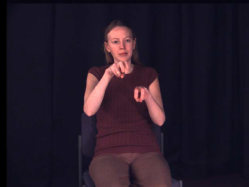
\includegraphics[width=0.25\textwidth]{capitulos/metodologia/imagens/asllvd_example_front}
    }%
    % \hfill
    \subcaptionbox{Vista lateral \label{subfig:asllvd-example-side}
    }{
        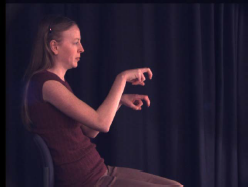
\includegraphics[width=0.25\textwidth]{capitulos/metodologia/imagens/asllvd_example_side}
    }%
    % \hfill
    \subcaptionbox{Vista da face \label{subfig:asllvd-example-close}
    }{
        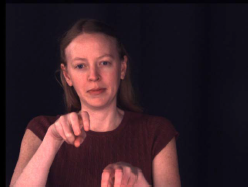
\includegraphics[width=0.25\textwidth]{capitulos/metodologia/imagens/asllvd_example_close}
    }%
    \nomefonte[p. 2]{athitsos-2008-asllvd}
    \label{fig:asllvd-example}
\end{figure}


Para que fosse possível extrair \textit{features} no formato de parâmetros fonológicos a partir das amostras do \acrshort{asllvd}, que são compostas essencialmente de sequências de vídeos com frames em RGB, tivemos que realizar um processo de duas etapas.

Na primeira, realizamos a estimativa das coordenadas dos esqueletos dos indivíduos para duas das perspectivas fornecidas para as amostras, os quais foram combinados em seguida para compor um esqueleto tridimensional final. A saída dessa etapa deu origem ao \textit{dataset} intermediário denominado ASL-Skeleton3D. 
Na segunda, aplicamos um conjunto de operações algébricas sob esse esqueleto tridimensional para finalmente computar nossos parâmetros fonológicos, processo esse que originou o \textit{dataset} ASL-Phono.

% Para computar parâmetros fonológicos a partir dos frames das amostras do \acrshort{asllvd}, compostos essencialmente de imagens RGB bidimensionais, precisamos realizar um processo de duas etapas: primeiro, estimamos as coordenadas 2D dos esqueletos dos sinalizadores para duas câmeras distintas, frame-a-frame, e as combinamos para projetar um esqueleto no espaço 3D -- isso deu origem ao \textit{dataset} intermediário chamado ASL-Skeleton3D; em seguida, aplicamos um conjunto de operações algébricas sob o esqueleto 3D para calcular os parâmetros fonológicos -- o que gerou assim o nosso \textit{dataset} final chamado ASL-Phono.

Esse processo de extração de \textit{features} envolveu alguns desafios relevantes, dentre os quais podemos enumerar:

\begin{enumerate}
    \item Definição de uma estratégia para representar indivíduos no espaço tridimensional utilizando apenas frames de vídeo bidimensionais simples, bem como para contornar a ausência de perspectivas ou a baixa qualidade de algumas dessas amostras;

    \item Estabelecimento de um subconjunto inicial de atributos fonológicos capaz de capturar e representar variações significativas na articulação dos sinais, e que ao mesmo tempo pudessem ser modelados computacionalmente nessa primeira iteração da abordagem proposta.

    \item Identificação de técnicas matemáticas e medidas antropométricas que pudessem fundamentar a modelagem e o cálculo desses atributos.

    \item Demanda por recursos computacionais significativos para processar duas perspectivas distintas para cada uma das quase 10.000 amostras contidas em cada \textit{dataset}. Em média, isso consumiu cerca de 40 horas contínuas de processamento distribuído com GPUs e gerou mais de 1 TB de dados cada vez que os \textit{datasets} precisaram ser re-gerados.
\end{enumerate}


% Dataset 3d
\input{capitulos/metodologia/datasets_3d}

% Dataset phono
\input{capitulos/metodologia/datasets_phono}

% PREPARAÇÃO DO DATASET -------------------------------------------

\section{Preparação dos dados}
\label{sec:metodologia-preparacao-dados}

Para tornar as amostras do ASL-Phono compatíveis com a entrada dos modelos que serão utilizados mais adiante, aplicamos uma transformação simples que consiste em codificar seus atributos fonológicos como blocos ou ``palavras'' únicas, mais compactas. Ou seja, ao invés de utilizar como entrada sequências de frames que contêm propriedades aninhadas, adotamos aqui sequências de blocos compactos que codificam a mesma informação de uma forma mais amigável a modelos sequenciais.

Observe na \autoref{tab:codificacao-bloco} um exemplo deste processo. Na primeira linha, temos os valores originais das propriedades providas para o frame de uma amostra do ASL-Phono; na segunda linha, geram-se acrônimos a partir desses atributos para realizar uma primeira compactação -- mas que não é um passo necessariamente obrigatório; na terceira linha, temos um bloco ou palavra única gerada pela composição desses acrônimos; finalmente, na última linha, temos o exemplo de uma sequência desses blocos.

\input{capitulos/metodologia/tabelas/codificacao_bloco}


% RESAMPLING DO DATASET -------------------------------------------

Conforme observa-se pela \autoref{tab:dataset-phono-stats}, o ASL-Phono apresenta um desbalanceamento no número de amostras disponíveis por sinal. Em média, há 3,68 amostras disponíveis por sinal porém, enquanto alguns sinais têm apenas 1 amostra, outros apresentam um número atípico de 59. Isso poderia influenciar o desempenho dos modelos utilizados adiante, uma vez que durante o treinamento alguns sinais seriam favorecidos e, outros, penalizados. 

Por conta disso, aplicamos dois procedimentos para reduzir o desbalanceamento desses dados: primeiro, eliminamos os sinais com apenas 1 amostra, uma vez que esse número é insuficiente para que o modelo seja capaz de aprender e generalizar acerca desses sinais, sobretudo quando o \textit{dataset} é particionado durante o treinamento; segundo, realizamos uma reamostragem do \textit{dataset} para equilibrar o número de amostras.

Observe na \autoref{subfig:dataset-resampling-antes} um perfil detalhado dos dados antes da reamostragem. É possível perceber que o número de amostras é bastante disperso pelo eixo horizontal do gráfico: por exemplo, 726 sinais apresentam 2 amostras disponíveis; seguidos por 552 sinais com 4 amostras; mas, no outro extremo, temos que apenas um número muito pequeno de sinais (entre 1 e 3) apresentam um grande número de amostras disponíveis (entre 13 e 59), respectivamente.

\begin{figure}[ht!]
    \centering
    \caption{
        \textmd{Número de amostras disponíveis por sinal (\subref{subfig:dataset-resampling-antes}) antes da reamostragem e (\subref{subfig:dataset-resampling-depois}) após a reamostragem do ASL-Phono. Por exemplo, lê-se que 726 sinais possuem 2 amostras disponíveis antes da reamostragem.}
    }
    \subcaptionbox{\label{subfig:dataset-resampling-antes}}{
        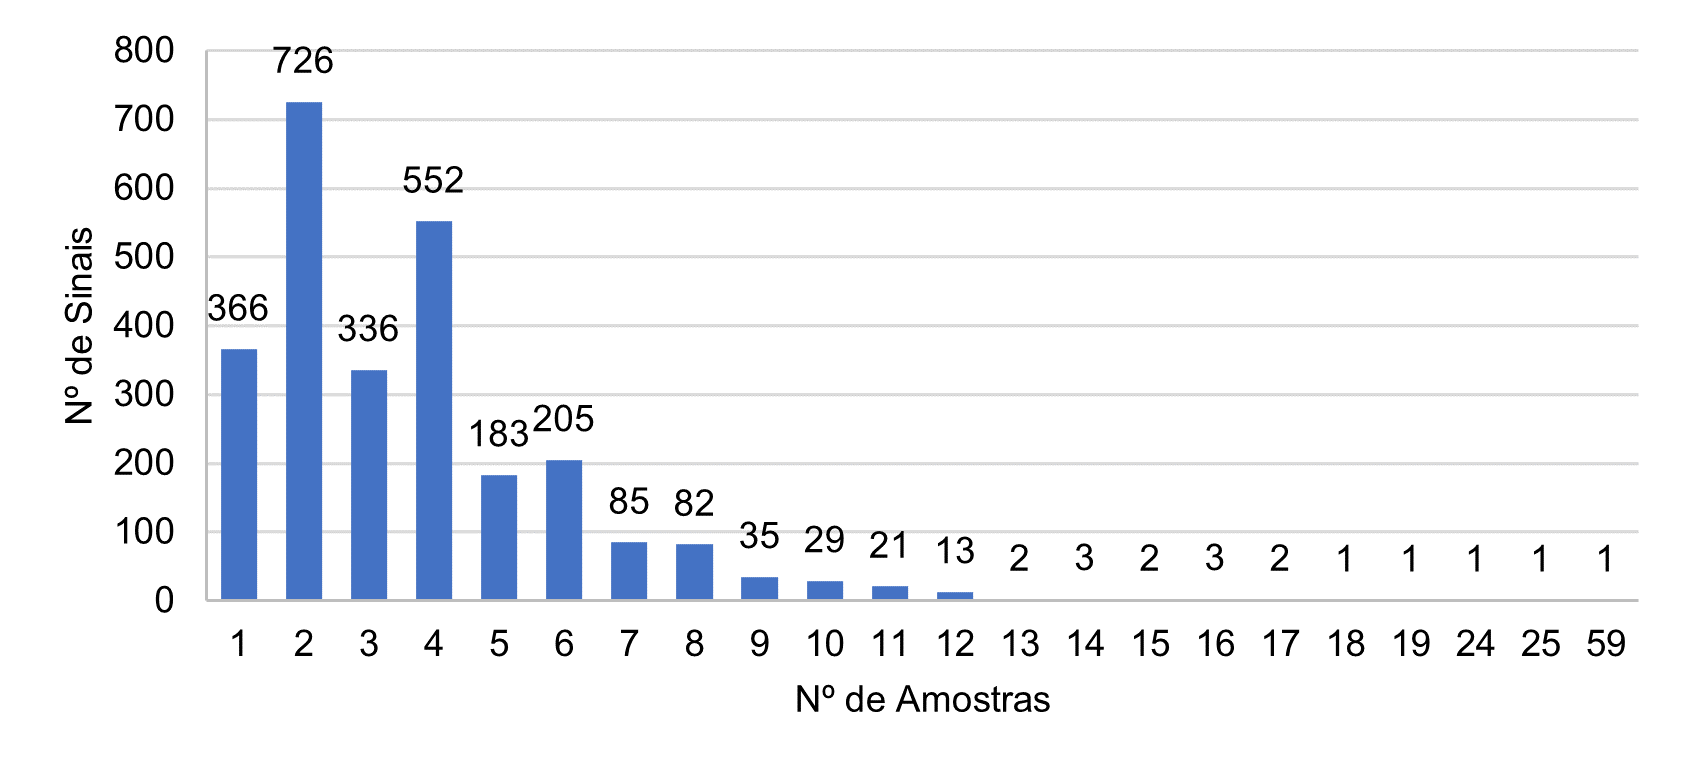
\includegraphics[height=6cm]{capitulos/metodologia/imagens/dataset_resampling_antes}
    }%
    \hspace{1cm}
    \subcaptionbox{\label{subfig:dataset-resampling-depois}}{
        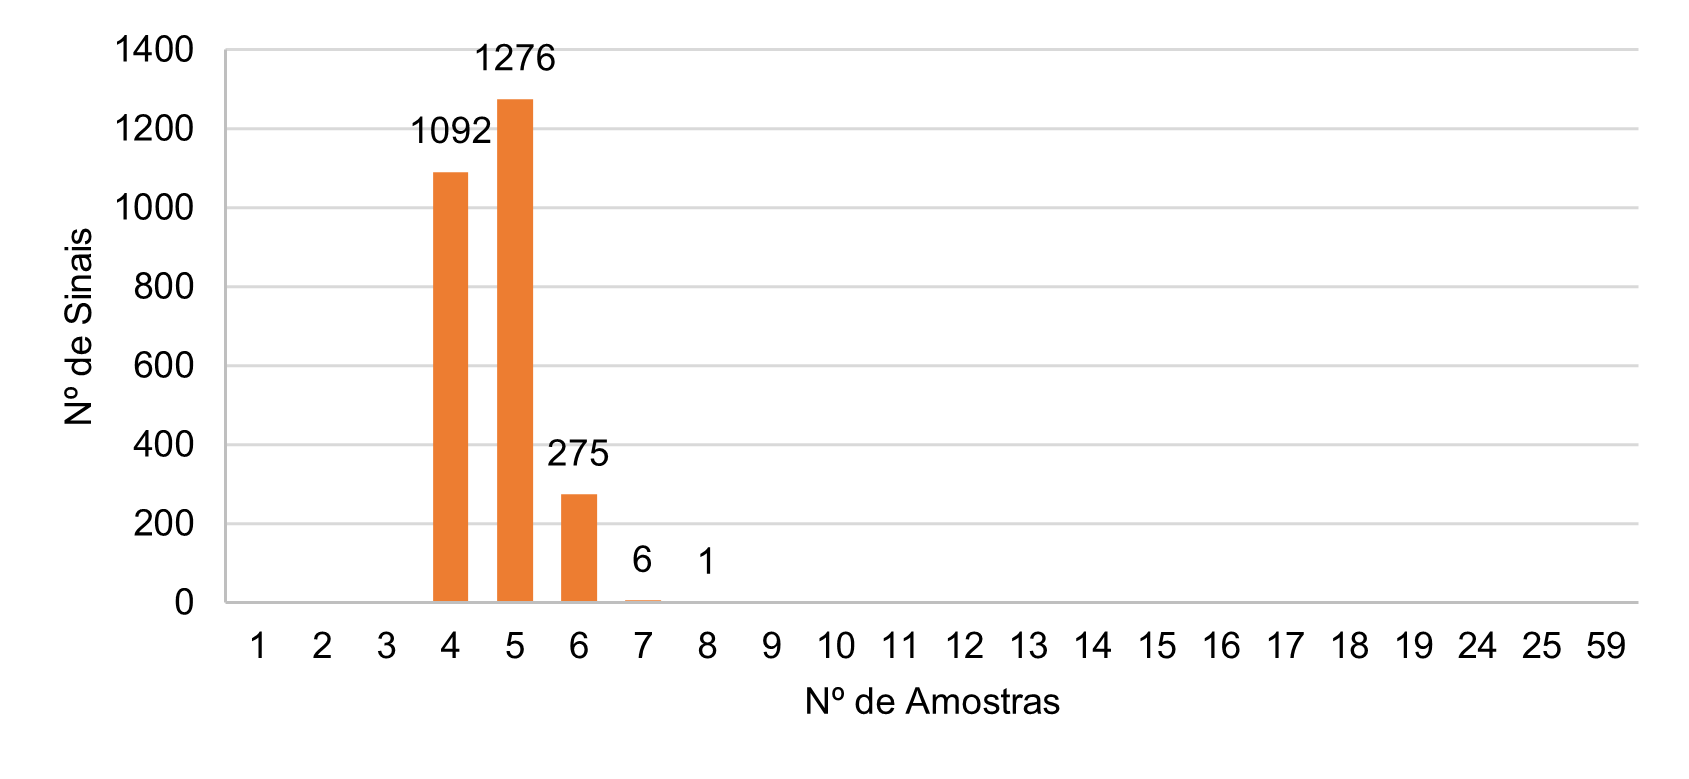
\includegraphics[height=6cm]{capitulos/metodologia/imagens/dataset_resampling_depois}
    }%
    \nomefonte{}
    \label{fig:dataset-resampling}
\end{figure}

Aplicamos então uma reamostragem \textit{naive random under-sampling} (ou sub-amostragem aleatória ingênua, que reduz o número de amostras através de uma seleção aleatória de algumas delas para os sinais que estão super-representados) seguida de uma \textit{naive random over-sampling} (ou sobre-amostragem aleatória ingênua, que replica aleatoriamente algumas das amostras existentes para os sinais que estão sub-representados).
Para estabelecer o novo número de amostras por sinal \(x'\), utilizamos a \autoref{eqn:resampling-target}: 

\begin{equation}
    \label{eqn:resampling-target}
    x' = round( \overline{a} + \ln(x) )
\end{equation}

Onde \(\overline{a}\) refere-se ao número médio de amostras por sinal no \textit{dataset} e \(x\) é o número de amostras para aquele sinal. Observe na \autoref{subfig:dataset-resampling-depois} como os dados ficaram organizados após a reamostragem. Em resumo, a equação faz com que o número de amostras por sinal se concentre mais uniformemente a partir do valor da média.

\section{Preparação dos modelos}
\label{sec:metodologia-preparacao-modelos}

% Uma vez que temos um \textit{dataset} com atributos fonológicos processados, agora podemos prosseguir com a preparação das features e dos modelos para reconhecimentos dos sinais utilizando a abordagem proposta.


% Experimento
%   Preparação das features (asl-phono -> palavras)
%       Transformação das sequências no dataset: frames -> palavras
%       Justificativa??
%   Preparação dos modelos (Transformer, LSTM, GRU, etc) -- por modelo
%       Arquitetura + Parâmetros
%       lr scheduler, optimizer, loss function
%       Busca de parâmetros (dimensionar os modelos/parâmetros)



% SELEÇÃO DOS MODELOS -------------------------------------------

Tomando como referência a discussão introduzida na \autoref{sec:modelos-sequenciais}, adotaremos nos experimentos deste trabalho três das principais arquiteturas utilizadas em tarefas de \acrfull{nlp}: o \textit{Encoder-Decoder} em uma versão com \acrfull{lstm} e em outra com \acrfull{gru}, e também o \textit{Transformer}.

% Os parâmetros para treinamento dos modelos foram selecionados com base na discussão apresentada por \citeonline{goodfellow-2016-deep-learning}, a qual aborda de forma prática temas como definição de métricas, modelos de base, otimização de parâmetros, entre outros para tal finalidade.

Para estabelecer os parâmetros dessas arquiteturas, as estratégias de otimização e treinamento, bem como as métricas a serem utilizadas nos experimentos, nos fundamentamos pela discussão apresentada por \citeonline{goodfellow-2016-deep-learning}.
Dessa forma, o algoritmo de otimização será definido como o \acrfull{sgd} com \textit{momentum} de 0,9. Ele será combinado a uma estratégia de redução da taxa de aprendizagem por um fator de 0,2 sempre que o valor da perda calculada sobre os dados de validação atingir um platô por 5 épocas seguidas. A função de perda, por sua vez, será a \textit{Cross-Entropy Loss} (ou Perda de Entropia Cruzada) e os \textit{batches} de dados possuirão tamanho de 50 amostras. Por fim, os dados serão particionados numa proporção de 15\% para validação, 15\% para testes e o restante para treinamento dos modelos.

% Dessa forma, utilizamos como algoritmo de otimização o \acrfull{sgd} com \textit{momentum} de 0,9. Ele foi combinado com uma estratégia de redução da taxa de aprendizagem por um fator de 0,2 sempre que o valor da perda calculada sobre os dados de validação atinge um platô por 5 épocas seguidas. A função de perda utilizada, por sua vez, foi a \textit{Cross-Entropy Loss} (ou Perda de Entropia Cruzada). Além disso, adotamos \textit{batches} com tamanho de 50 amostras e particionamos o \textit{dataset} numa proporção de 15\% para validação, 15\% para testes e o restante para treinamento dos modelos.


Realizamos uma otimização de parâmetros do tipo \textit{Grid Search} para identificar a melhor configuração para cada um dos modelos em nosso contexto. 

% TODO: detalhar arquitetura do seq2seq + lstm:
Para o modelo \textit{Encoder-Decoder} com \acrshort{lstm} utilizamos ...

% TODO: detalhar arquitetura do seq2seq + gru:
Para o \textit{Encoder-Decoder} com \acrshort{gru}, por sua vez, utilizamos ...

No caso do \textit{Transformer}, não aplicamos nenhuma customização e adotamos a arquitetura original introduzida por \cite{vaswani-2017-transformer} -- que consiste de \textit{embeddings} com dimensões de 512, camadas ocultas com dimensões de 2048, 6 camadas, 8 cabeças e \textit{dropout} de 0,1.
Realizamos uma otimização da taxa de aprendizagem para esse modelo utilizando a estratégia de \textit{grid search} com validação cruzada de 5 \textit{folds} por 50 épocas. O resultado, ilustrado na \autoref{fig:otim_lr_transformer}, nos mostra que o valor que melhor minimiza a perda é 0,1.

\figura[]
    {fig:otim_lr_transformer}
    {capitulos/metodologia/imagens/otim_lr_transformer}
    {height=4.0cm}
    {Otimização da taxa de aprendizagem com relação à perda calculada para o \textit{Transformer}. LR refere-se à taxa de aprendizagem (ou \textit{learning rate}).}
    {}

\figura[]
    {fig:otim_lr_encdec_lstm}
    {capitulos/metodologia/imagens/otim_lr_encdec_lstm}
    {height=4.0cm}
    {Otimização da taxa de aprendizagem com relação à perda calculada para o \textit{Encoder-Decoder (LSTM)}. LR refere-se à taxa de aprendizagem (ou \textit{learning rate}).}
    {}


\figura[]
    {fig:otim_lr_encdec_gru}
    {capitulos/metodologia/imagens/otim_lr_encdec_gru}
    {height=4.0cm}
    {Otimização da taxa de aprendizagem com relação à perda calculada para o \textit{Encoder-Decoder (GRU)}. LR refere-se à taxa de aprendizagem (ou \textit{learning rate}).}
    {}

O código-fonte utilizado nos experimentos deste trabalho está disponível no endereço indicado abaixo\footnote{
    Disponível em \url{https://www.cin.ufpe.br/~cca5/sl-nlp}.
}.



% \cite{goodfellow-2016-deep-learning}

% --------
% A reasonable choice of optimization algorithm is SGD with momentum with a decaying learning rate (popular decay schemes that perform better or worse on different problems include decaying linearly until reaching a fixed minimum learning rate, decaying exponentially, or decreasing the learning rate by a factor of 2–10 each time validation error plateaus).

% - optimizer: SGD
%     nesterov: False
%     momentum: 0.9
% --------
% Loss function

% - criterion: CrossEntropyLoss

% --------
% Early stopping should be used almost universally.

% - training_args:
%     max_epochs: 50
%     batch_size: 50
%     lr: 0.01
%     test_size: 0.15
%     valid_size: 0.15
%     early_stopping:
%         patience: 10
%         threshold: 10e-4
%         threshold_mode: rel
%     gradient_clipping:
%         gradient_clip_value: 0.5
%     lr_scheduler: 
%         policy: ReduceLROnPlateau
%         factor: 0.2
%         patience: 5

% --------
% Learning rate - apresentar graficos?
% - learning rate (grid search)


% --------
% - dimensões dos modelos

%     Transformer (selecionamos as dimensões do modelo clássico \cite{vaswani-2017-transformer})
%         embedding_size: 512
%         hidden_size: 2048
%         num_layers: 6
%         dropout: 0.1
%         num_heads: 8

    
\section{Preparação dos experimentos}
\label{sec:metodologia-preparacao-experimentos}

Os parâmetros para treinamento dos modelos foram selecionados com base na discussão apresentada por \citeonline{goodfellow-2016-deep-learning}, a qual aborda de forma prática temas como definição de métricas, modelos de base, otimização de parâmetros, entre outros para tal finalidade.

Dessa forma, utilizamos como algoritmo de otimização o \acrfull{sgd} com \textit{momentum} de 0,9. Ele foi combinado com uma estratégia de redução da taxa de aprendizagem por um fator de 0,2 sempre que o valor da perda calculada sobre os dados de validação atinge um platô por 5 épocas seguidas. A função de perda utilizada, por sua vez, foi a \textit{Cross-Entropy Loss} (ou Perda de Entropia Cruzada). Além disso, adotamos \textit{batches} com tamanho de 50 amostras e particionamos o \textit{dataset} numa proporção de 15\% para validação, 15\% para testes e o restante para treinamento dos modelos.

% TODO: detalhar arquitetura do seq2seq + lstm:
Para o modelo \textit{Encoder-Decoder} com \acrshort{lstm} utilizamos ...

% TODO: detalhar arquitetura do seq2seq + gru:
Para o \textit{Encoder-Decoder} com \acrshort{gru}, por sua vez, utilizamos ...

No caso do \textit{Transformer}, não aplicamos nenhuma customização e adotamos a arquitetura original introduzida por \cite{vaswani-2017-transformer} -- que consiste de \textit{embeddings} com dimensões de 512, camadas ocultas com dimensões de 2048, 6 camadas, 8 cabeças e \textit{dropout} de 0,1.
Realizamos uma otimização da taxa de aprendizagem para esse modelo utilizando a estratégia de \textit{grid search} com validação cruzada de 5 \textit{folds} por 50 épocas. O resultado, ilustrado na \autoref{fig:otim_lr_transformer}, nos mostra que o valor que melhor minimiza a perda é 0,1.

\figura[]
    {fig:otim_lr_transformer}
    {capitulos/metodologia/imagens/otim_lr_transformer}
    {height=4.0cm}
    {Otimização da taxa de aprendizagem com relação à perda calculada para o \textit{Transformer}. LR refere-se à taxa de aprendizagem (ou \textit{learning rate}).}
    {}

\figura[]
    {fig:otim_lr_encdec_lstm}
    {capitulos/metodologia/imagens/otim_lr_encdec_lstm}
    {height=4.0cm}
    {Otimização da taxa de aprendizagem com relação à perda calculada para o \textit{Encoder-Decoder (LSTM)}. LR refere-se à taxa de aprendizagem (ou \textit{learning rate}).}
    {}


\figura[]
    {fig:otim_lr_encdec_gru}
    {capitulos/metodologia/imagens/otim_lr_encdec_gru}
    {height=4.0cm}
    {Otimização da taxa de aprendizagem com relação à perda calculada para o \textit{Encoder-Decoder (GRU)}. LR refere-se à taxa de aprendizagem (ou \textit{learning rate}).}
    {}

O código fonte utilizado nos experimentos está disponível no endereço indicado abaixo\footnote{
    Disponível em \url{https://www.cin.ufpe.br/~cca5/sl-nlp}.
}.



% \cite{goodfellow-2016-deep-learning}

% --------
% A reasonable choice of optimization algorithm is SGD with momentum with a decaying learning rate (popular decay schemes that perform better or worse on different problems include decaying linearly until reaching a fixed minimum learning rate, decaying exponentially, or decreasing the learning rate by a factor of 2–10 each time validation error plateaus).

% - optimizer: SGD
%     nesterov: False
%     momentum: 0.9
% --------
% Loss function

% - criterion: CrossEntropyLoss

% --------
% Early stopping should be used almost universally.

% - training_args:
%     max_epochs: 50
%     batch_size: 50
%     lr: 0.01
%     test_size: 0.15
%     valid_size: 0.15
%     early_stopping:
%         patience: 10
%         threshold: 10e-4
%         threshold_mode: rel
%     gradient_clipping:
%         gradient_clip_value: 0.5
%     lr_scheduler: 
%         policy: ReduceLROnPlateau
%         factor: 0.2
%         patience: 5

% --------
% Learning rate - apresentar graficos?
% - learning rate (grid search)


% --------
% - dimensões dos modelos

%     Transformer (selecionamos as dimensões do modelo clássico \cite{vaswani-2017-transformer})
%         embedding_size: 512
%         hidden_size: 2048
%         num_layers: 6
%         dropout: 0.1
%         num_heads: 8

    

% Avaliação experimental
\chapter{Avaliação experimental}
\label{cap:avaliacao}

Nos capítulos anteriores, introduzimos a abordagem proposta e a metodologia utilizada para preparar e executar os experimentos neste trabalho.
Neste capítulo, portanto, analisaremos os resultados apresentados por esses experimentos.
Faremos isso em duas partes: 
primeiro, discutiremos os resultados coletadas para cada um dos modelos utilizados; em seguida, compararemos esses resultados com aqueles obtidos por outras pesquisas em \acrfull{slr} que também adotaram o \acrfull{asllvd} como base de análise, mas que seguiram por abordagens distintas.

\section{Análise dos resultados}
\label{sec:avaliacao-resultados}

A \autoref{tab:resultados-modelos} apresenta o desempenho dos modelos utilizados nos experimentos deste trabalho, respectivamente o \textit{Encoder-Decoder} implementado com \acrshort{lstm}, o \textit{Encoder-Decoder} implementado com \acrshort{gru} e o \textit{Transformer}.
Para cada modelo, são listadas as métricas\footnote{
    Uma vez que o reconhecimento de sinais consiste numa classificação multi-classes, os valores das métricas binárias de precisão, \textit{recall} e \textit{F1-score} foram consolidados utilizando-se a média ponderada pelo número de amostras em cada classe.
} de acurácia, precisão, \textit{recall} e \textit{F1-score}, bem como o erro médio calculado.

% precisao, recall, f1 calculados com média ponderada entre classes (weighted average)
% precisao, recall, f1 consistentes com acurácia (justificar)

\input{capitulos/avaliacao/tabelas/resultados-modelos}

% %FIXME: [cz] eu sei que na proxima secao vc vai apresentar a comparação com os trabalhos relacionados, mas aqui senti falta de um baseline que pudesse comparar com a abordagem original qual foi a melhora usando a estratégia linguistica em relacao a usar somente as imagens --> [cca5] um pouco mais a frente eu acabo discutindo essas diferenças (que basicamente giram em torno do nível semântico que aqui é maior e faz mais sentido perante a língua)

Primeiramente, observa-se que os modelos baseados na arquitetura \textit{Encoder-Decoder} apresentaram resultados muito semelhantes entre si, apesar de ainda não muito expressivos de um modo geral.
% De um modo geral, percebe-se entre os modelos baseados na arquitetura \textit{Encoder-Decoder} resultados muito semelhantes entre si, mas não muito expressivos.
Dentre eles, percebe-se também que a versão implementada utilizando codificador e decodificador baseados em redes \acrshort{gru} obteve uma pequena vantagem em comparação àquela que utilizou redes \acrshort{lstm} -- ao passo que a primeira alcançou uma acurácia de 46,98\%, a segunda obteve 45,99\%.
O valor das demais métricas e do erro médio computado para ambos os casos replicaram esse mesmo comportamento da acurácia e reforçam tal análise.

Por outro lado, quando analisados os resultados do \textit{Transformer} observa-se um desempenho bastante expressivo com uma acurácia de 100,00\%, a qual excede aquelas apresentadas pelos \textit{Encoder-Decoders} e é reiterada consistentemente pelo valor das demais métricas e também da perda computada.

Isso nos remete à argumentação de \citeonline{wolf-2020-transformers,jurafsky-2022-speech-lang-processing} citada na \autoref{sec:am-ap}, que afirma que essa arquitetura tem se mostrado extremamente bem-sucedida entre tarefas de \acrfull{nlp}, superando arquiteturas como as \acrshortpl{rnn}. Exatamente por isso, elas são atualmente dominantes nessa área.

No contexto deste trabalho, acredita-se que alguns motivos particulares contribuíram para os resultados acima.
Em primeiro lugar, entende-se que a escolha pelo uso da abordagem linguística dos sinais nos permitiu trabalhar num nível semântico muito mais elevado do que seria possível fazer com dados brutos como os pixels de imagens RGB ou coordenadas aleatórias no espaço. Conforme discutido no \autoref{cap:metodos}, essa é uma abordagem comum em tarefas envolvendo linguagem no \acrshort{nlp} e que permite produzir \textit{features} de melhor qualidade para ensinar os modelos acerca da estrutura dessas línguas.

Em segundo lugar, a representação introduzida aqui foi capaz de transformar um conjunto de canais linguísticos complexos dos sinais do \acrshort{asllvd}, em \textit{features} discretas (ou ``palavras'', como aqui as denominamos) mais simples e bem definidas a serem consumidas pelos modelos.
Isso deu origem a um vocabulário que, por sua vez, é muito menos complexo do que aqueles com os quais arquiteturas como o \textit{Transformer} foram originalmente projetadas para lidar. Além disso, nesse processo foi selecionado um número menor de atributos fonológicos da língua de sinais e isso também contribuiu para tornar nosso vocabulário ainda mais compacto.

Dessa forma, entende-se que a combinação desse conjunto de \textit{features} semanticamente mais coerentes e simplificadas, com a utilização de um modelo robusto no processamento de linguagens como o \textit{Transformer}, foram fatores que conduziram ao desempenho favorável acima.
Contudo, para os \textit{Encoder-Decoders} esse desempenho foi mais modesto.

% encoder-decoders com desempenho proximo, mas GRU com uma leve vantagem
% transformer com desempenho muito superior
% - provavelmente pela combinação: 
%   - o transformer é muito robusto e projetado para lidar problemas muito complexos de linguagem. / ele está super-dimensionado para o problema em questão?
%   - essa abordagem super-simplifica o problema da língua de sinais produzindo um conjunto de features predominantemente discretas, como se tivéssemos um vocabulário de texto --> em oposição ao que ocorre quando opta-se por abordagens de visão computacional com dados brutos











% -> Precision is the fraction of detections reported by the model that were correct, while recall is the fraction of true events that were detected.
% In many cases, we wish to summarize the performance of the classifier with a single number rather than a curve. To do so, we can convert precision p and recall r into an F-score (or F-measure) given by:
%     F = 2pr / p + r.
% Another option is to report the total area lying beneath the PR curve.



% averaging techniques applicable to multiclass classification -------------
% (https://towardsdatascience.com/comprehensive-guide-on-multiclass-classification-metrics-af94cfb83fbd)
% weighted: accounts for class imbalance by computing the average of binary metrics weighted by the number of samples of each class in the target. If 3 (precision scores) for 3 classes are: Class 1 (0.85), class 2 (0.80), and class 3 (0.89), the weighted average will be calculated by multiplying each score by the number of occurrences of each class and dividing by the total number of samples.


Com o objetivo de estabelecer um comparativo entre os resultados deste trabalho e aqueles apresentados por outras pesquisas na área de \acrfull{slr}, selecionamos alguns estudos que também utilizaram o \acrshort{asllvd} como referência em seus experimentos, os quais introduziremos brevemente a seguir:

% Para comparar os resultados obtidos neste trabalho, selecionamos algumas pesquisas que também adotaram o \acrshort{asllvd} para realizar o reconhecimento dos sinais.
% A maioria deles, no entanto, limita-se aos segmentos das mãos para isso e também utiliza como dados de entrada coordenadas 3D ou imagens RGB dos frames das amostras, as quais são processadas por técnicas de visão computacional.
% Além disso, eles comumente selecionam subconjuntos menores de sinais ao invés de considerar o \textit{dataset} completo, como fizemos aqui -- isso contribui para acurácias maiores mas limitá-os perante o contexto real de aplicação da língua.


\begin{itemize}
    % tipo de dado bruto?
    % recorte de mãos x corpo inteiro?

    \item \textbf{\citeonline{theodorakis-2014-dynamic-static}}: utiliza técnicas não-supervisionadas e também \acrfull{hmm} para gerar subunidades de movimento e pausa (chamadas 2-S-U) que são utilizadas para reconhecer os sinais.
          Para isso, os autores processaram os frames das amostras concentrando-se apenas nas mãos dos indivíduos e selecionaram um subconjunto de 97 sinais do \acrshort{asllvd}.
          % processa frames de vídeo / foco nas mãos

    \item \textbf{\citeonline{lim-2016-bhof}}: introduz a técnica de \acrfull{bhof}, que gera histogramas do fluxo óptico das mãos dos indivíduos a partir dos frames das amostras.
          Em seus experimentos, os autores selecionaram um subconjunto pequeno contendo apenas 20 sinais do \acrshort{asllvd}.

          Além disso, esse trabalho apresenta um comparativo dos resultados do \acrshort{bhof} com aqueles obtidos pelas técnicas \acrfull{mei}, \acrfull{mhi}, \acrfull{pca} e \acrfull{hof} para esse mesmo subconjunto de sinais.
          % processa frames de vídeo / recorta as mãos (remove outras partes)

    \item \textbf{\citeonline{metaxas-2018-linguistically}}: combina diferentes técnicas para produzir uma variedade de features que se referem a configuração de mão inicial e final; número de mãos envolvidas; distância entre mãos; coordenadas 3D do corpo, face, mãos e braços; e contato das mãos com o corpo. Elas são utilizadas como entrada para um modelo baseado em \acrfull{hcorf} para reconhecer um subconjunto selecionado de 350 sinais do \acrshort{asllvd}.
          % extrai features: a) handshapes (start and end); b) number of hands; c) 3D upper body locations, movements of the hands and arms, and distance between the hands; d) facial features (include 66 points from 3D estimates for the forehead, ear, eye, nose, and mouth regions, and their velocities across frames) and head movements; e) contact (extracted from our 3D face and upper body movement estimation, and relate to the possibilities of the hand touching specific parts of the head or body).
          % processa frames de video para extrair features de nivel maior / considera mix de features e coordenadas 3D

    \item \textbf{\citeonline{lim-2019-isolated-slr-cnn-hei}}: introduz uma representação chamada \acrfull{hei} que, por sua vez, também concentra-se nas mãos dos indivíduos e é utilizada como entrada para uma rede \acrfull{cnn}.
          Aqui os autores adotam o mesmo subconjunto de 20 sinais definidos por \citeonline{lim-2016-bhof} acima.
          % processa frames de vídeo / recorta as mãos

    \item \textbf{\citeonline{amorim-2019-stgcn-sl}}: utiliza grafos para modelar a dimensão espacial das coordenadas 2D do corpo dos indivíduos bem como a relação temporal dos seus movimentos, os quais são fornecidos como entrada para uma rede \acrfull{stgcn}.
          Os autores avaliam os resultados para o mesmo subconjunto de 20 sinais definidos por \citeonline{lim-2016-bhof}, mas também para o \acrshort{asllvd} inteiro.
          % coordenadas 2D para grafos / corpo inteiro
\end{itemize}


De um modo geral, observa-se que a maioria dos estudos acima aborda a tarefa de \acrlong{slr} através do processamento de dados brutos, geralmente frames RGB ou coordenadas 2D ou 3D, conforme discutimos ao longo da \autoref{sec:slr}.
Apesar de em alguns casos esses dados serem utilizados para gerar features intermediárias -- como subunidades de movimento e pausa, imagens de fluxo óptico ou de energia de movimento, histogramas, grafos, entre outras -- estas, por sua vez, apresentam um nível semântico muito menos informativo quanto à língua de sinais e sua linguística propriamente ditas do que aquelas que introduzimos neste trabalho.

Uma outra observação importante é a de que parte desses trabalhos concentra-se apenas nas mãos dos indivíduos e isso nos remete a um dos problemas de abordagem do \acrshort{slr} discutidos na \autoref{sec:slr-desafios}. Como resultado disso, canais referentes a traços linguísticos relevantes como, por exemplo, expressões não-manuais, locação das mãos e movimentos do corpo, acabam sendo desconsiderados.

Além disso, percebe-se que todos esses trabalhos modelam vocabulários que correspondem a subconjuntos muito pequenos do \acrshort{asllvd}, conforme discutimos na \autoref{sec:slr-breve-panorama}.
Esses subconjuntos, por sua vez, representam menos de 13\% do vocabulário total disponibilizado por esse \textit{dataset}, que consiste de 2.745 sinais.

Apesar de compreendermos que todos esses fatores têm por objetivo simplificar o tamanho e a complexidade do escopo abordado por essas pesquisas, é inevitável ressaltar após a discussão realizada ao longo deste trabalho, que esses recortes distanciam a língua de sinais de seu contexto real de uso e, consequentemente, limitam a produção de contribuições significativas para a área de \acrshort{slr}.

% insights [ASLLVD tem 2.745 sinais]
% considerações importantes
% - são pesquisas que adotam abordagens que utilizam dados brutos (RGB, coordenadas)
% - muitas delas adotam recortes das mãos apenas
% - não consideram a fonologia
% - utilizam um número de sinais limitados, com o intuito de reduzir a complexidade -- consequentemente
%     - isso contribui para que eles obtenham acurácias maiores
%     - contudo, limita o problema perante o contexto real -- uma vez que a afasta da realidade da língua


\input{capitulos/avaliacao/tabelas/comparacao-resultados}


Uma vez introduzido esse debate, vamos analisar os resultados listados na \autoref{tab:comparacao-resultados}.
Ao comparar as pesquisas acima com os modelos utilizados em nossos experimentos, como um todo, vemos que os \textit{Encoder-Decoders} apresentaram um desempenho bastante mediano com relação aos demais. Ao mesmo tempo em que sua acurácia por volta de 46,00\% foi capaz de superar técnicas como \acrshort{pca}, \acrshort{hei}, \acrshort{mei} e \acrshort{mhi}, outras técnicas como \acrshort{hcorf}, \acrshort{bhof}, \acrshort{hof} e \acrshort{stgcn} conseguiram superar essa marca alcançando valores de até 93,30\%.
A acurácia de 100,00\% do \textit{Transformer}, por sua vez, superou de forma consistente o desempenho apresentado pelas demais técnicas na tabela.

Se compararmos apenas os estudos que modelaram features referentes ao corpo inteiro do indivíduo ao invés de apenas suas mãos -- ainda que indiretamente, através de dados brutos -- temos uma perspectiva diferente. \citeonline{metaxas-2018-linguistically} e \citeonline{amorim-2019-stgcn-sl} se enquadram nesses critérios e, pela tabela, vemos que ambas as técnicas de \acrshort{hcorf} e \acrshort{stgcn} superaram os resultados das implementações de \textit{Encoder-Decoders} utilizadas em nossos experimentos.


% - ao comparar nossos experimentos com todos os trabalhos acima, de uma forma generalizada, vemos que o desempenho dos encoder-decoders (por volta dos 46%) foi mediano com relação aos demais (que em vários deles alcançaram marcas de 70%, 85% e até 93,30%)
% - no caso do transformer, seu desempenho posicionou-se superior aos demais trabalhos

Em contrapartida, essa análise é ainda diferente se considerarmos apenas estudos que modelaram um vocabulário com todos os sinais do \acrshort{asllvd}, que seria uma complexidade equivalente à que abordamos em nossos experimentos.
Pela tabela, apenas \citeonline{amorim-2019-stgcn-sl} registraram resultados sob essas condições, o qual foi de 16,48\% para sua técnica \acrshort{stgcn}. 
Esse número é bem inferior às acurácias de 45,99\% e 46,98\% alcançadas pelas implementações de \textit{Encoder-Decoders} utilizadas em nossos experimentos. Quando comparado ao \textit{Transformer}, por sua vez, é constatada uma margem de diferença ainda mais expressiva para esse número.

% ------------
% - contudo, considerando que maioria deles modela apenas vocabulários pequenos [que correspondem em média a 2% do vocabulário disponível no ASLLVD (que é o que utilizamos aqui) e não ultrapassam 13% dele], nota-se que 
% - no entanto, se considerarmos apenas aqueles trabalhos que consideraram todos os sinais do ASLLVD (que seria um vocabulário de complexidade equivalente à nossa), percebemos que mesmo os encoder-decores apresentaram um salto importante, ficando em torno dos 46% de acurácia (quando até então observava-se por volta de 16%)
%   - se olharmos o transformer, esse salto é ainda mais expressivo





% Algumas comparações (HEI - Hand Energy Image x MEI, MHI) com ASLLVD
% 2020 - Amorim, Macedo, Zanchettin - Spatial-Temporal Graph Convolutional Networks for Sign Language Recognition
%                         accuracy
%     (tudo)              16.48
%     (20 sinais)         61.04

% 2016 - Lim, Tan, Tan - Block-based histogram of optical flow for isolated sign language recognition
%     (20 sinais)
%         MHI             10.00
%         MEI             25.00
%         PCA             45.00
%         HOF             70.00
%         > BHOF          85.00


% 2019 - Lim et al - Isolated sign language recognition using Convolutional Neural Network hand modelling and Hand Energy Image
%     (20 sinais - duas mãos)
%         > Proposed HEI  31.50
%         MEI             25.00
%         MHI             10.00 
%         MEI + MHI       20.00

% 2014 - Dilsizian et al - A New Framework for Sign Language Recognition based on 3D Handshape Identification and Linguistic Modeling
% https://aclanthology.org/L14-1096/
%     >                  81.76

% 2014 - Theodorakis, Pitsikalis, Maragos - Dynamic–static unsupervised sequentiality, statistical subunits and lexicon for sign language recognition
%     (97 signs)
%     > 2-S-U            63.15

% 2018 - Metaxas, Dilsizian, Neidle - Linguistically-driven Framework for Computationally Efficient and Scalable Sign Recognition
% https://par.nsf.gov/servlets/purl/10065369
%     > (350 signs)      93.3




% Considerações finais
\chapter{Considerações finais}
\label{cap:consideracoes-finais}

Introduzimos ao longo deste trabalho uma abordagem que concentra-se nos atributos linguísticos da língua de sinais para realizar o seu reconhecimento.
Apesar dessa ser uma estratégia comum entre tarefas de \acrfull{nlp}, ela difere-se da abordagem que tem sido utilizado pela maioria das pesquisas em \acrfull{slr} que, por sua vez, concentra-se principalmente no processamento de dados brutos como pixels RGB ou coordenadas.

% Isso é diferente do que observamos para grande parte das pesquisas realizadas nas últimas décadas na área de \acrfull{slr} principalmente porque retiramos o foco do processamento de dados brutos e problemas que estão sob domínio da \acrfull{cv} e o colocamos no processamento da língua acima como \acrfull{nlp} propriamente dito.

Dessa maneira, transicionamos o foco do domínio da \acrfull{cv} para o domínio do \acrshort{nlp}, permitindo que os modelos aplicados aprendessem acerca da estrutura linguística em vez das relações entre pixels e coordenadas, por exemplo.
Pelos resultados apresentados no \autoref{cap:avaliacao}, percebemos que essa abordagem apresentou uma eficácia bastante satisfatória quando combinada com o modelo \textit{Transformer} que, por sua vez, é uma arquitetura amplamente utilizada atualmente e bem-sucedida ao lidar com tarefas envolvendo linguagens.

% intro
% contributions and takeaways
% difficulties and limitations/challenges?
% future works




\bookmarksetup{startatroot}% 


% ----------------------------------------------------------
% ELEMENTOS PÓS-TEXTUAIS
% ----------------------------------------------------------
\postextual


% ----------------------------------------------------------
% BIBLIOGRAFIA
% ----------------------------------------------------------
%\bibliographystyle{abntexalfenglish} %caso seja em inglês, retire o comentário desta linha

% \renewcommand{\bibname}{REFER\^ENCIAS}
%\renewcommand{\bibname}{Bibliography}
% \addbibresource{sample.bib}
\bibliography{referencias}


% ----------------------------------------------------------
% APENDICES
% ----------------------------------------------------------
% força para que não exiba subtítulos em apêndices no sumário
\begin{apendicesenv}
  \addtocontents{toc}{\protect\setcounter{tocdepth}{1}}
  \makeatletter
  \addtocontents{toc}{%
    \begingroup
    \let\protect\l@chapter\protect\l@section
    \let\protect\l@section\protect\l@subsection
  }
  \makeatother

  % Imprime uma página indicando o início dos apêndices
  % \partapendices
  % Apendices

%%coloca o identificador do anexo/apendice somente na primeira página
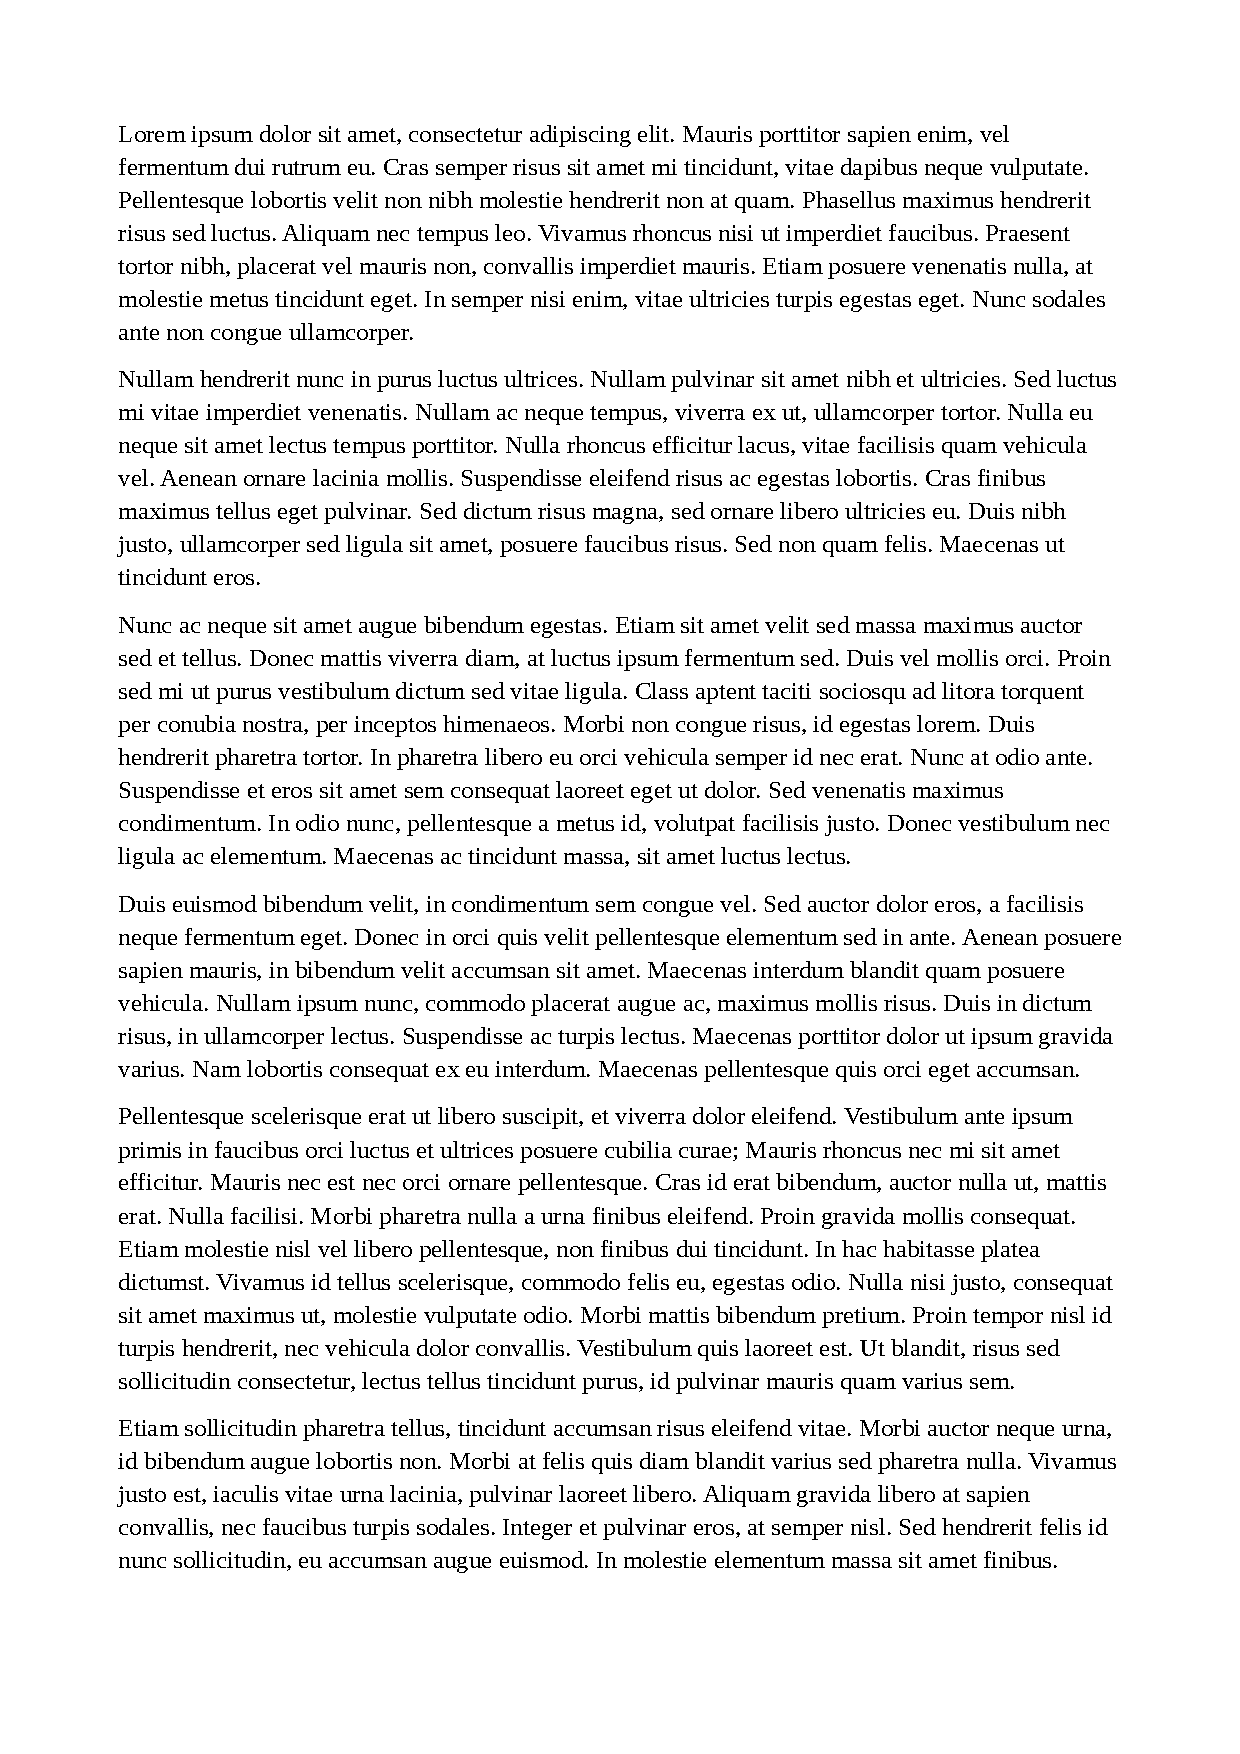
\includepdf[pages={1},scale=0.8,pagecommand=\chapter{Texto Texto Texto Texto}\label{apen:apendiceA}]{appendix/apendiceA}
\includepdf[pages={2-},scale=0.80,pagecommand={}]{appendix/apendiceA}

%%coloca o identificador do anexo/apendice somente na primeira página

\includepdf[pages={1},scale=0.80,pagecommand=\chapter{Texto Texto Texto}\label{apen:apendiceB}]{appendix/apendiceB}


%%coloca o identificador do anexo/apendice somente na primeira página
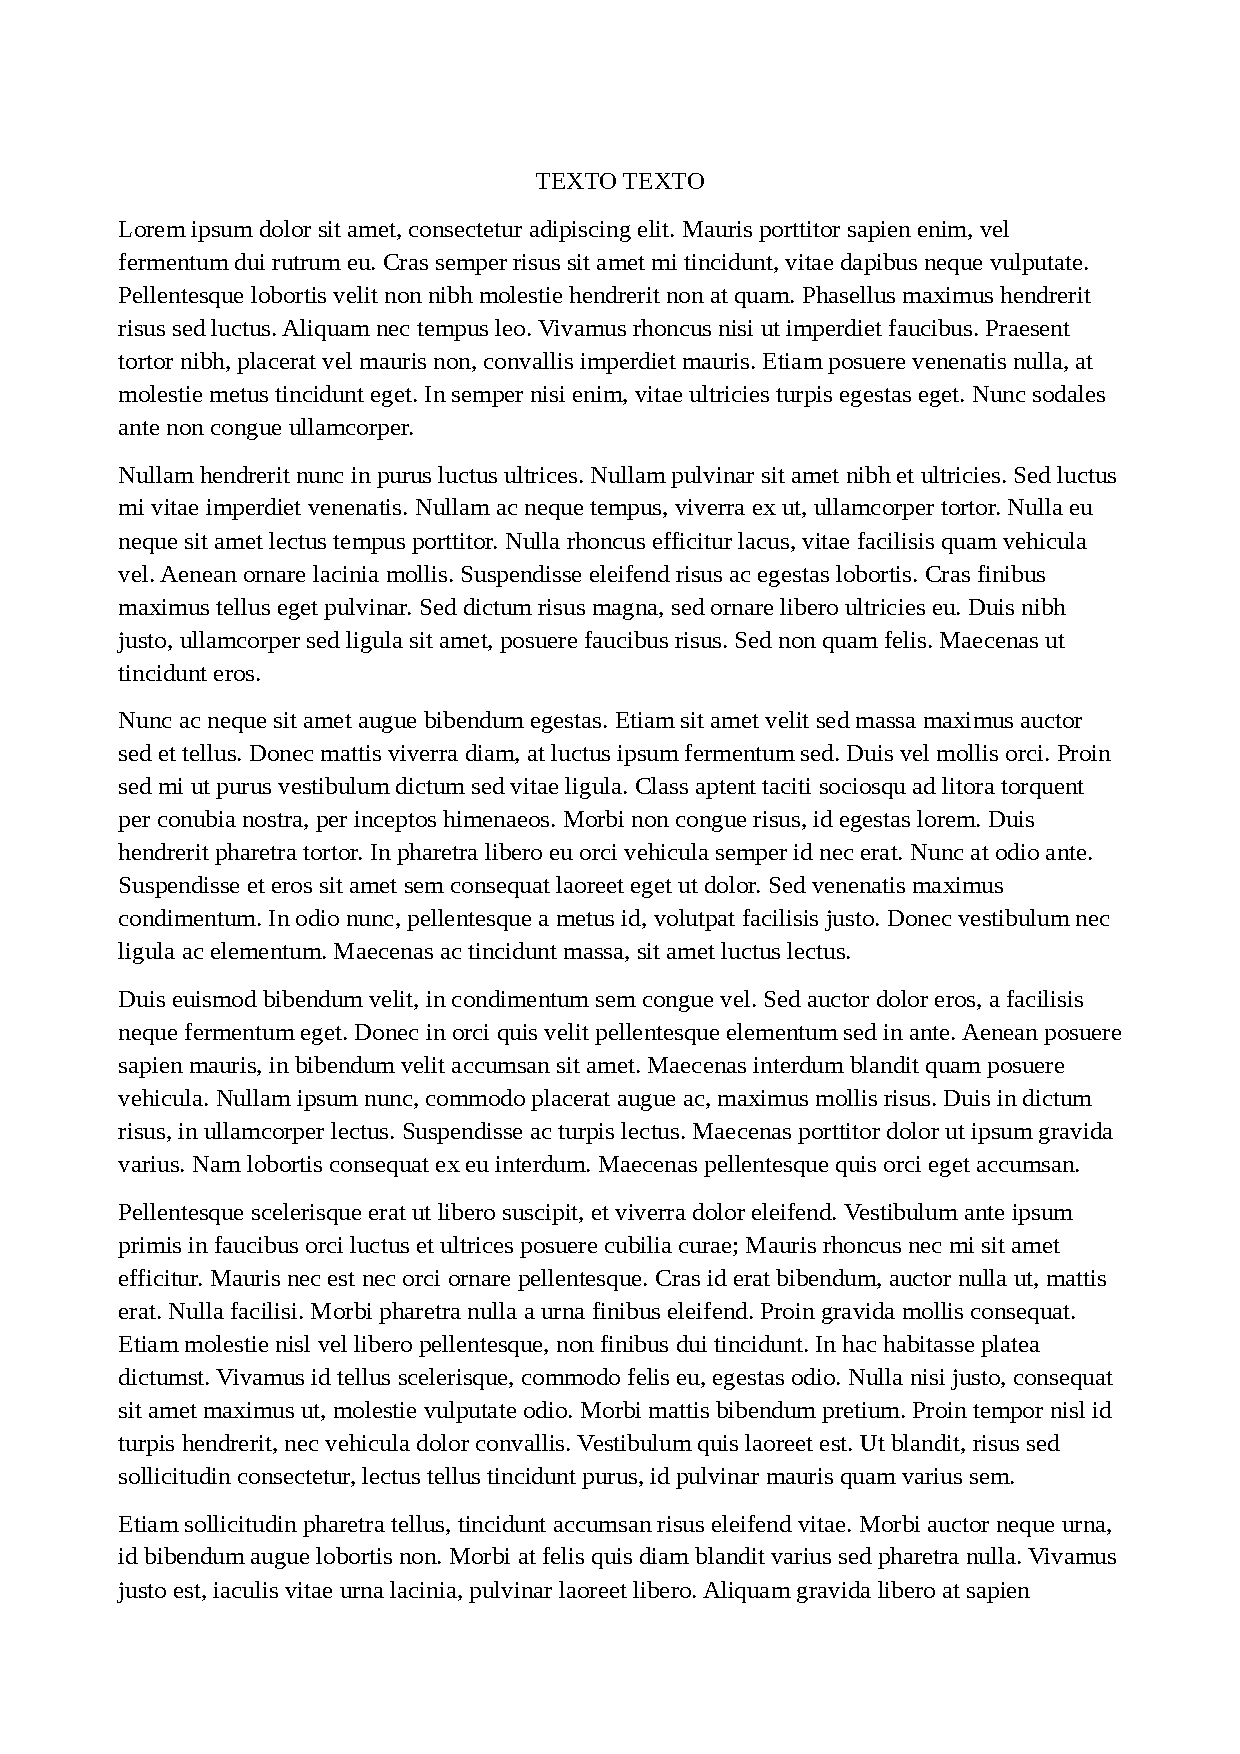
\includepdf[pages={1},scale=0.80,pagecommand=\chapter{Texto Texto}\label{apen:apendiceC}]{appendix/apendiceC}
\includepdf[pages={2},scale=0.80,pagecommand={}]{appendix/apendiceC}




  \addtocontents{toc}{\endgroup}
\end{apendicesenv}



% ----------------------------------------------------------
% ANEXOS
% ----------------------------------------------------------
% força para que não exiba subtítulos em apêndices no sumário
\begin{anexosenv}
  \addtocontents{toc}{\protect\setcounter{tocdepth}{1}}
  \makeatletter
  \addtocontents{toc}{%
    \begingroup
    \let\protect\l@chapter\protect\l@section
    \let\protect\l@section\protect\l@subsection
  }
  \makeatother
  % Imprime uma página indicando o início dos apêndices
  % \partapendices
  % Anexos

%%coloca o identificador do anexo/apendice somente na primeira página
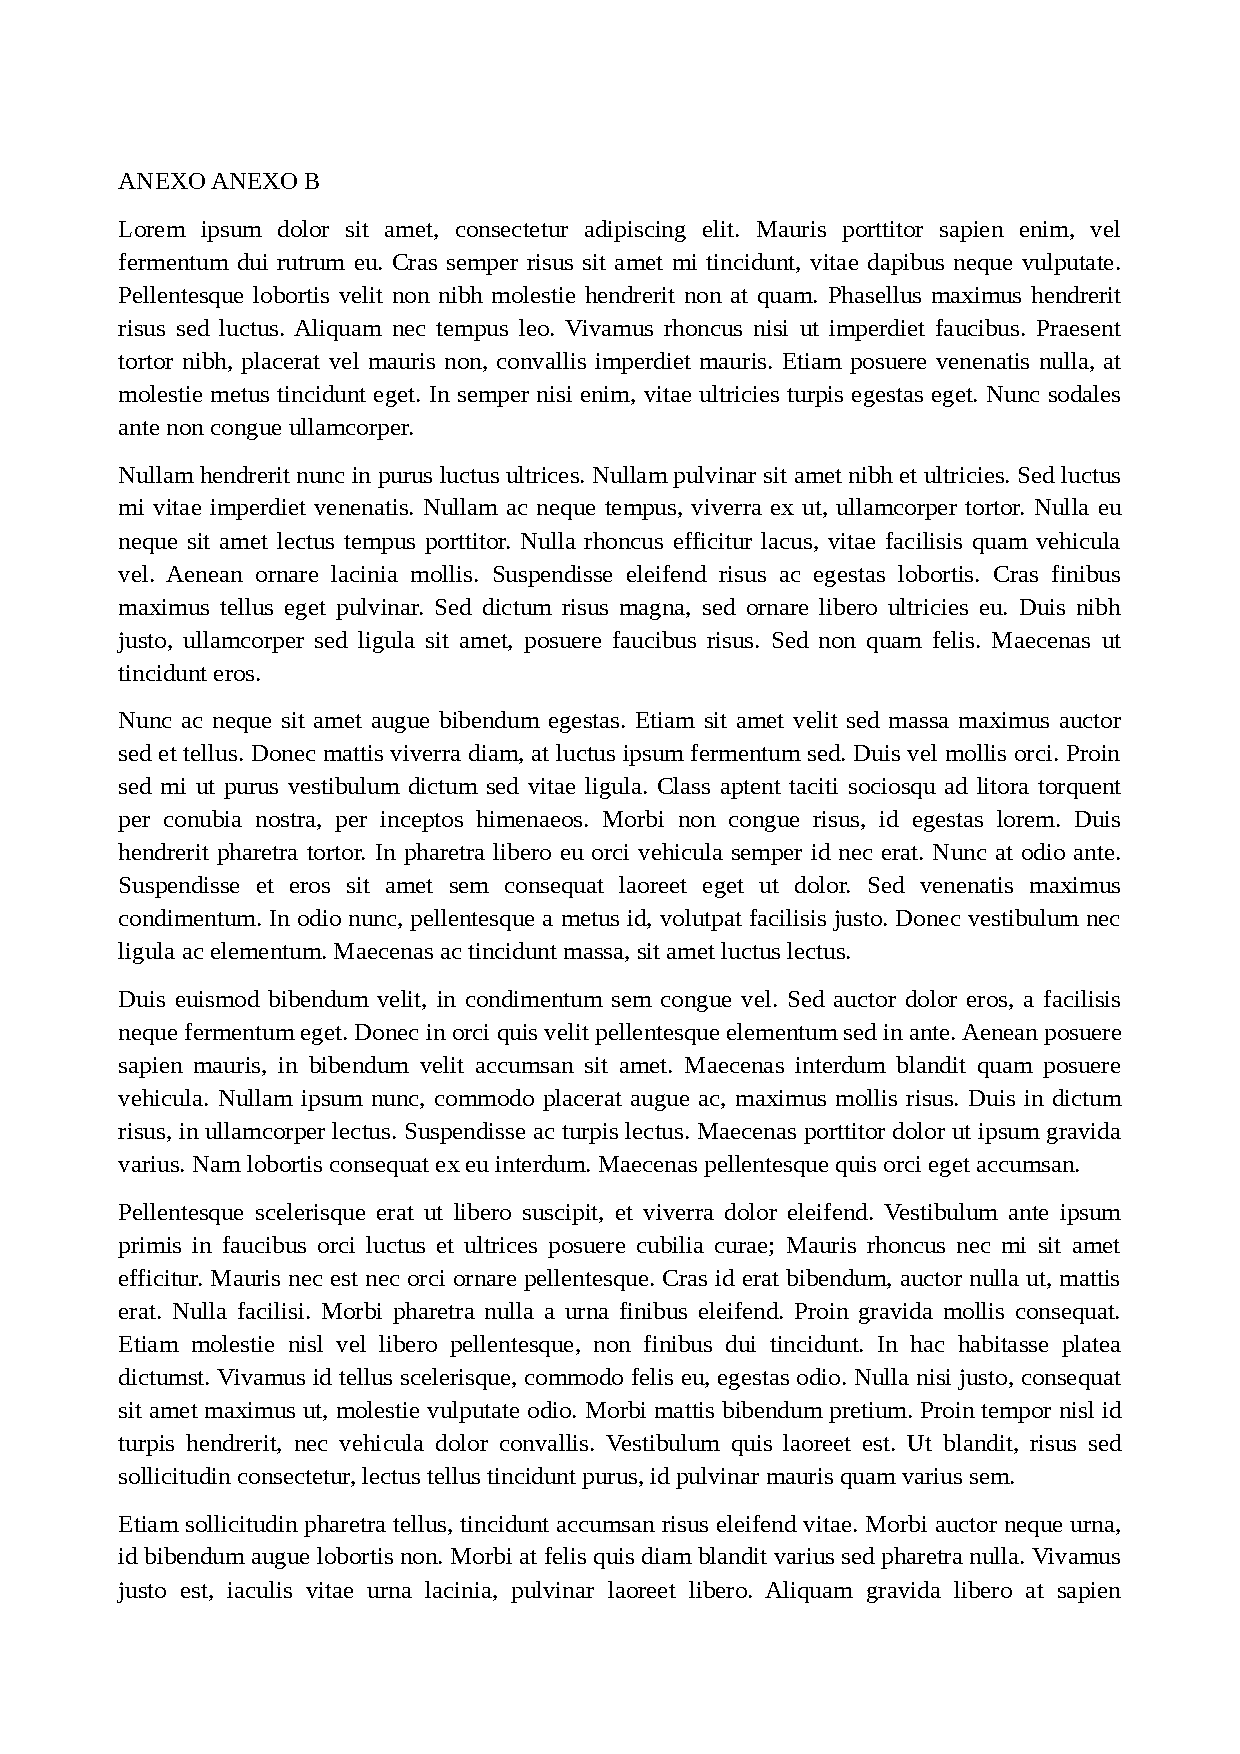
\includepdf[pages={1},scale=0.8,pagecommand=\chapter{Texto Texto Texto Texto}\label{anex:anexob}]{anexos/anexoB}
\includepdf[pages={2-},scale=0.80,pagecommand={}]{anexos/anexoB}

%%coloca o identificador do anexo/apendice somente na primeira página
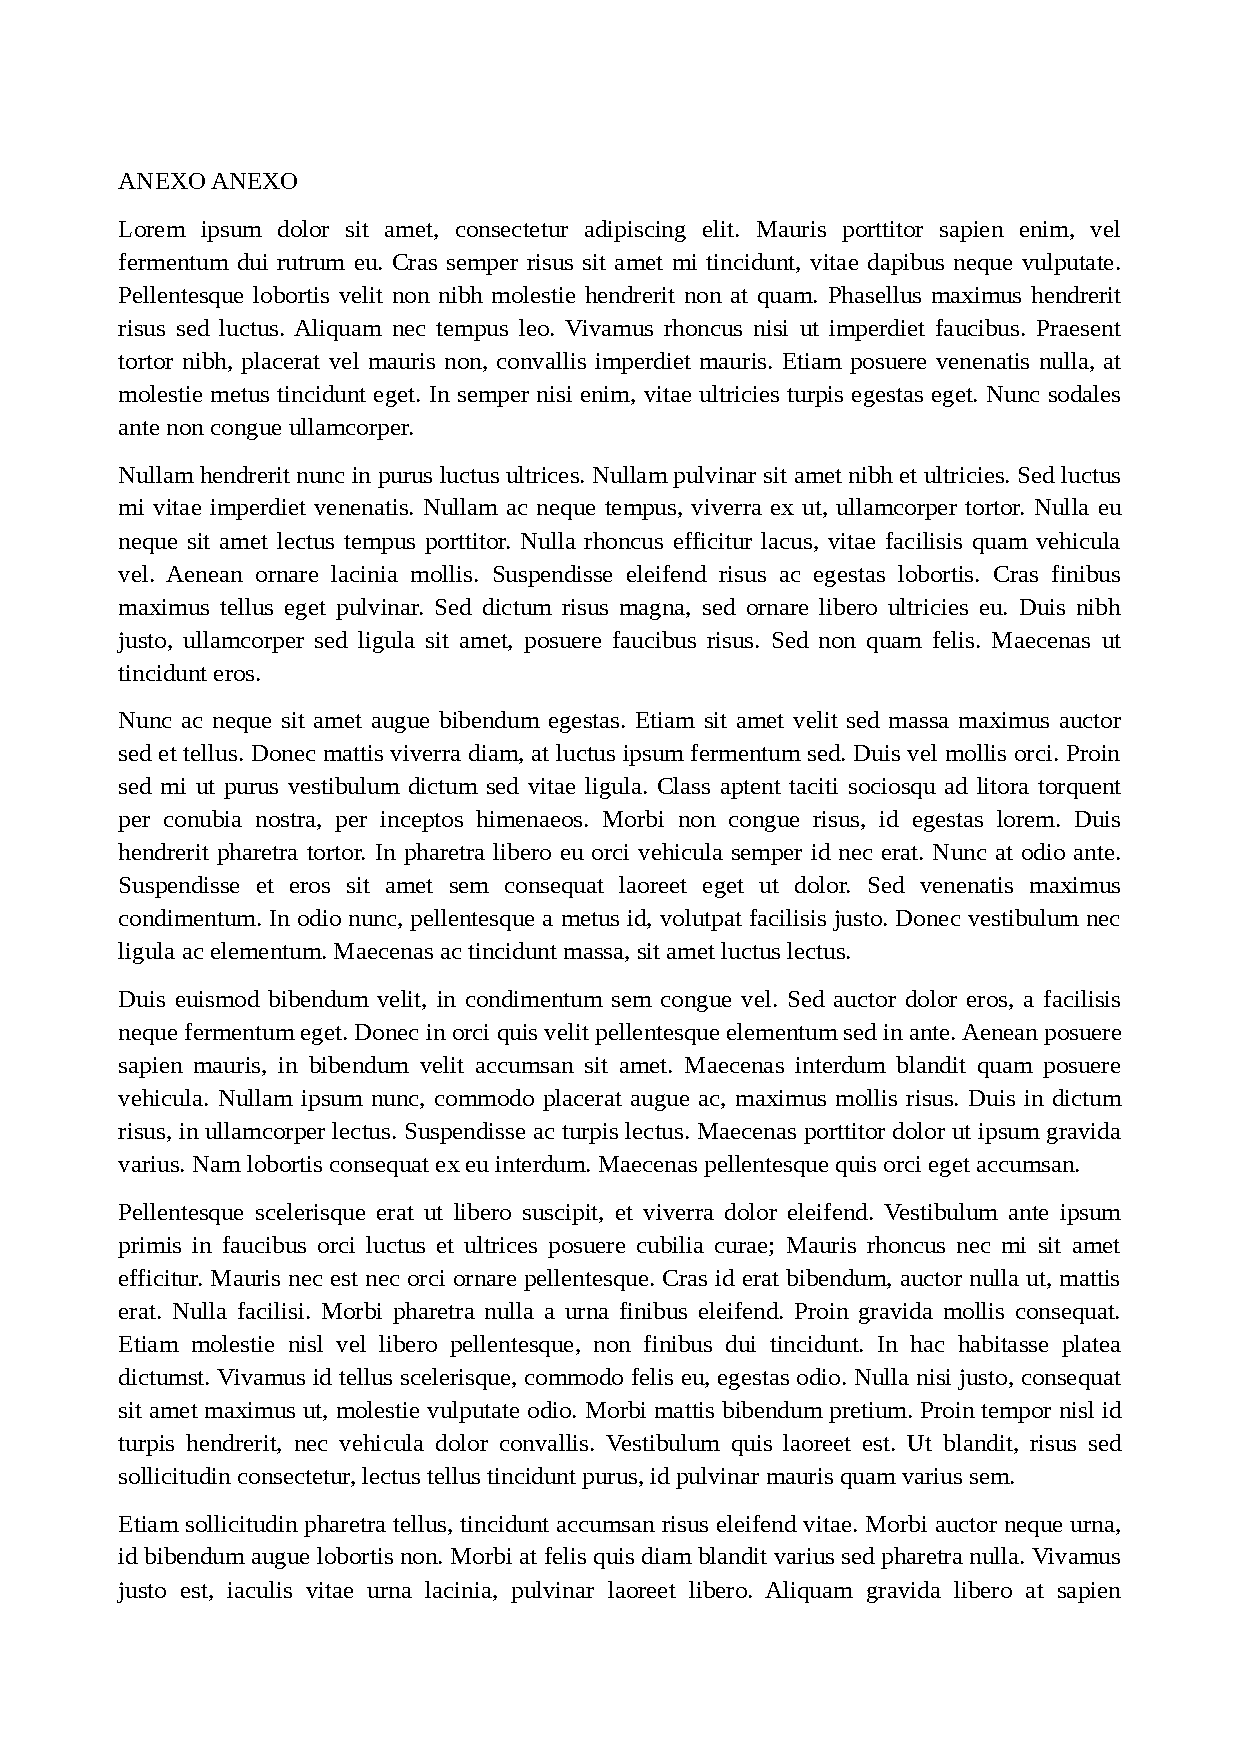
\includepdf[pages={1},scale=0.8,pagecommand=\chapter{Texto Texto Texto Texto}\label{anex:anexoa}]{anexos/anexoA}
\includepdf[pages={2-},scale=0.80,pagecommand={}]{anexos/anexoA}


  \addtocontents{toc}{\endgroup}
\end{anexosenv}


% ----------------------------------------------------------
\printindex

\end{document}
